\documentclass[12pt,a4paper,halfparskip,headsepline,bibtotocnumbered]{scrreprt}

% ========== Pakete einbinden ==========
\usepackage[utf8]{inputenc}          % um Umlaute direkt eingeben zu können
\usepackage[T1]{fontenc}             % für "modernere" Schriftkodierung
\usepackage[ngerman]{babel}          % Sprachanpassungen für neue Deutsche Rechtschreibung
\usepackage[intlimits]{amsmath}      % für erweiterte mathematische Konstrukte
\usepackage{amsfonts}                % für erweiterte mathematische Schriften
\usepackage{amssymb}                 % für erweiterten Symbolvorrat
\usepackage[sc]{mathpazo}            % Schriftart Palatino
\usepackage{textcomp}                % für erweiterten Text-Symbolvorrat
\usepackage{typearea}                % für die Berechnung der Seitenründer
\usepackage{scrpage2}                % für Kopf- und Fußzeilen
\usepackage{array}                   % für erweiterte Tabellensatzmöglichkeiten
\usepackage{enumerate}               % für komfortablere Aufzählungen
\usepackage{titlesec}                % für Kontrolle der Abschnittüberschriften
\usepackage[amsmath, thmmarks]{ntheorem} % für Definitionen, Sätze, ...
\usepackage{graphicx}
\usepackage{framed}
\usepackage{lmodern}
\usepackage{blindtext}
\usepackage{pdfpages}
\usepackage{url}
\usepackage{enumitem}
\usepackage[Algorithmus]{algorithm}
\usepackage[noend]{algpseudocode}
\usepackage{multirow}
\usepackage{diagbox}

% Spezialpakete
\usepackage{fp}
\usepackage{tikz}
\usepackage{xcolor}
% TikZ-Bibliotheken
\usetikzlibrary{arrows}
\usetikzlibrary{shapes}
\usetikzlibrary{decorations.pathmorphing}
\usetikzlibrary{decorations.pathreplacing}
\usetikzlibrary{decorations.shapes}
\usetikzlibrary{decorations.text}
\usetikzlibrary{calc}

\usepackage{shadethm}

% ========== Layout ==========
\typearea{12}
\linespread{1.5}
\titleformat{\section}{\normalfont\normalcolor\Large\bfseries\centering}%
 {\S\,\thesection}{.66em}{}
\newcommand{\subsectiontitel}[1]{\raisebox{0.6ex}{\rule{12pt}{0.4pt}}%
 \hspace*{0.2cm}\textit{#1}\hspace*{0.2cm}\raisebox{0.6ex}{\rule{12pt}{0.4pt}}}
\titleformat{\subsection}[block]{\normalfont\normalcolor\centering}{}{0em}{\subsectiontitel}

% ---------- Definitionen, Sätze, ... ----------

\makeatletter

\newtheoremstyle{nummermitklammern}%
 {\item[\rlap{\vbox{\hbox{\hskip\labelsep \theorem@headerfont
  (##2)\ ##1\theorem@separator}\hbox{\strut}}}]}%
 {\item[\rlap{\vbox{\hbox{\hskip\labelsep \theorem@headerfont
  (##2)\ ##1 (##3)\theorem@separator}\hbox{\strut}}}]}%
\makeatother

\theoremstyle{nummermitklammern}
\theorembodyfont{\rmfamily}
%\theoremsymbol{\ensuremath{\diamond}}
\newtheorem{defsatzusw}{}[section]
\newtheorem{definition}[defsatzusw]{Definition}
\newtheorem{bezeichnung}[defsatzusw]{Bezeichnung}
\newtheorem{bezeichnungen}[defsatzusw]{Bezeichnungen}
\newtheorem{voraussetzung}[defsatzusw]{Voraussetzung}
\newtheorem{voraussetzungen}[defsatzusw]{Voraussetzungen}
\newtheorem{satz}[defsatzusw]{Satz}


\newtheorem{lemma}[defsatzusw]{Lemma}
\newtheorem{algorithmus}[defsatzusw]{Algorithmus}
\newtheorem{korollar}[defsatzusw]{Korollar}
\newtheorem{folgerung}[defsatzusw]{Folgerung}
\newtheorem{hilfssatz}[defsatzusw]{Hilfssatz}
\newtheorem{proposition}[defsatzusw]{Proposition}
\newtheorem{bemerkung}[defsatzusw]{Bemerkung}
\newtheorem{bemerkungen}[defsatzusw]{Bemerkungen}
\newtheorem{beispiel}[defsatzusw]{Beispiel}
\newtheorem{beispiele}[defsatzusw]{Beispiele}
\theoremstyle{nonumberbreak}
\newtheorem{beweis2}{Beweis (Anfang):}
\theoremsymbol{\ensuremath{\square}}
\newtheorem{beweis}{Beweis:}
\newtheorem {fazit} {Fazit}



\definecolor{shadethmcolor}{rgb}{.9,.9,.9}   % Farbe des Hintergrundes 
\definecolor{shaderulecolor}{rgb}{0.0,0.0,1.0}   % Farbe des Rahmens
\setlength{\shadeboxrule}{1pt}   % Breite des Rahmens
\newshadetheorem{sthm}{lemma}
\newenvironment{thm}[1][]{%
  \definecolor{shadethmcolor}{rgb}{.9,.9,.9}%
  \definecolor{shaderulecolor}{rgb}{1.0,0.0,0.0}%
  \setlength{\shadeboxrule}{1pt}%
  \begin{sthm}[#1]%
}{\end{sthm}}

% ---------- Mathematik-Umgebungen ----------
\newenvironment{mathex}[1][LLLLLLLLLLLL]{
  \[%
  \newcolumntype{L}{>{\displaystyle\setlength{\arraycolsep}{4pt}}l}%
  \newcolumntype{C}{>{\displaystyle\setlength{\arraycolsep}{4pt}}c}%
  \newcolumntype{R}{>{\displaystyle\setlength{\arraycolsep}{4pt}}r}%
  \setlength{\arraycolsep}{1.5pt}%
  \begin{array}{>{\vspace*{1.3ex}}#1}%
}{
  \end{array}%
  \vspace*{-1.3ex}%
  \]%
  \ignorespacesafterend%
}

% ========== Abkuerzungen ==========
\newcommand{\N}{\mathbb{N}}
\newcommand{\Z}{\mathbb{Z}}
\newcommand{\Q}{\mathbb{Q}}
\newcommand{\R}{\mathbb{R}}
\newcommand{\C}{\mathbb{C}}
\newcommand{\G}{\mathbb{G}}
\newcommand{\F}{\mathbb{F}}
\renewcommand{\P}{\mathbb{P}}
\newcommand{\B}{\mathcal{B}}
\newcommand{\No}{\mathcal{N}}
\newcommand{\Det}{\text{Det}}
\newcommand{\Min}{\text{Min}}
\renewcommand{\O}{\mathcal{O}}
\newcommand{\I}{\mathcal{I}}
\newcommand{\J}{\mathcal{J}}
\newcommand{\p}{\mathfrak{p}}
\newcommand{\q}{\mathfrak{q}}
\renewcommand{\a}{\mathfrak{a}}
\renewcommand{\b}{\mathfrak{b}}
\newcommand{\A}{\mathfrak{A}}
\newcommand{\Bfrak}{\mathfrak{B}}
\makeatletter
\renewcommand{\i}{\text{\expandafter\@slowromancap\romannumeral 1@}}
\newcommand{\ii}{\text{\expandafter\@slowromancap\romannumeral 2@}}
\makeatother
\newcommand{\Kern}{\text{Kern}}
\newcommand{\Bild}{\text{Bild}}
\newcommand{\ggT}{\text{ggT}}
\newcommand{\kgV}{\text{kgV}}
\newcommand{\Aut}{\text{Aut}}
\newcommand{\Dim}{\text{Dim}}

% ========== Sonstiges ==========
\renewcommand{\emptyset}{\text{\usefont{OMS}{cmsy}{m}{n}\symbol{59}}}
\bibliographystyle{alpha}
\allowdisplaybreaks


\begin{document}

%===================================================================
% Titelseite
%===================================================================

\begin{titlepage}
	\centering
	%\includegraphics[width=0.5\textwidth]{RWTH_Logo.png}\par\vspace{1cm}
	\vspace*{2cm}
	{\Large\bfseries Extremale Gitter mit großen Automorphismen\par}
	\vspace{1cm}
	{\scshape\Large Masterarbeit\par}
	\vspace{2cm}
	{\Large\itshape von Simon Berger\par}
	\vfill
	Vorgelegt am Lehrstuhl D für Mathematik der RWTH-Aachen University\par 
	bei Prof. Dr. Gabriele Nebe (Erstgutachterin)\\ 
	und Prof. Dr. Markus Kirschmer (Zweitgutachter)\par
	\vfill

% Bottom of the page
	{\large \today\par}
\end{titlepage}

%===================================================================
% Inhaltsverzeichnis
%===================================================================

\tableofcontents

%===================================================================
% Kapitel 1: Einleitung
%===================================================================
\chapter{Einleitung}
Die Gittertheorie ist seit vielen Jahren ein wesentlicher Bestandteil der theoretischen Mathematik in Themengebieten wie der algebraischen Zahlentheorie und der Gruppentheorie. In der Anwendung sind oftmals Gitter von Interesse, welche besonders dichte Kugelpackungen liefern. Also Gitter, die im Vergleich zu ihrer Determinante ein möglichst großes Minimum besitzen. Die Klassifikation möglichst dichter Gitter stellt jedoch eine große Herausforderung dar.\par
H.-G. Quebbemann definiert in seiner Arbeit \cite{quebbemann} den Begriff eines \textit{modularen} Gitters und zeigt, dass die Thetareihen solcher modularen Gitter Modulformen einer bestimmten Gruppe sind. Diese Struktur erlaubt die Beschreibung sogenannter \textit{extremaler} modularer Gitter, welche innerhalb der Klasse der modularen Gitter eine maximale Dichte haben. Die Klassifikation extremaler Gitter ist eines der großen Forschungsgebiete aus der Gittertheorie. In dieser Arbeit wird versucht, extremale Gitter mithilfe ihrer Automorphismengruppen zu untersuchen und zu konstruieren.\par
Zunächst definieren wir dazu unsere grundlegenden Begriffe und werfen einen genaueren Blick auf die Dichte extremaler Gitter. Anschließend beschreiben wir modulare Gitter $L$ mit einer Struktur als gebrochene Ideale eines zyklotomischen Zahlkörpers $\Q(\zeta_m)$, sogenannte \textit{Ideal-Gitter}. Diese Struktur ist gegeben, falls $L$ einen Automorphismus $\sigma$ mit $\mu_\sigma = \Phi_m$ besitzt, sodass $\varphi(m) = \text{Dim}(L)$ gilt. Mithilfe dieser zusätzlichen Struktur lässt sich ein Algorithmus entwickeln, welcher zu gegebener Stufe, Determinante und Dimension eine vollständige Liste der Ideal-Gitter mit den festgelegten Parametern konstruiert. Dieser Algorithmus wurde von Michael Jürgens in \cite{juergens} beschrieben. Die einzelnen Schritte werden im Zuge dieser Arbeit genau untersucht und im Computer-Algebra-System \texttt{MAGMA} implementiert.\par
Im sich daran anschließenden Hauptteil der Arbeit erfolgt die Beschreibung extremaler modularer Gitter mit \textit{großem} Automorphismus. Hier gehen wir lediglich von den Voraussetzungen $\vert \sigma \vert = m$ und $\Phi_m \vert \mu_\sigma$ mit $\varphi(m) > \frac{\text{Dim}(L)}{2}$ aus. In diesem Falle induziert $\sigma$ ein Teilgitter $M := L \cap \Kern(\Phi_m(\sigma)) \perp L \cap \Kern(\frac{\mu_\sigma}{\Phi_m}(\sigma))$. DIe erste Komponente hat dabei eine Struktur als Ideal-Gitter und kann deshalb mit dem Algorithmus des vorherigen Kapitels leicht konstruiert werden; für die zweite Komponente benötigen wir weitere Theorie. Jürgens und Nebe untersuchen in \cite{juergens} und \cite{nebe} Gitterautomorphismen $\sigma$ mit Primzahlordnung $p$. Wie vorher induziert solch ein $\sigma$ ein Teilgitter $M := L \cap \Kern(\Phi_p(\sigma)) \perp L \cap \Kern(\Phi_1(\sigma))$, in diesem Falle lassen sich allerdings wichtige Einschränkungen an die Determinanten der Komponenten sowie an den Index von $M$ in $L$ zeigen. Die Informationen über Automorphismen von Primzahlordnung können anschließend verwendet werden, um mittels der Primteiler von $m$ auch Automorphismen allgemeinerer Ordnung zu untersuchen. Nebe wendet in \cite{nebe} diese Erkenntnisse an, um extremale unimodulare Gitter der Dimension $48$ mit großem Automorphismus zu klassifizieren. In dieser Arbeit wird die dortige Vorgehensweise auf $\ell$-modulare Gitter verallgemeinert und als Algorithmus zusammengefasst. Alle Voraussetzungen und Teilschritte werden dabei genau erläutert und in \texttt{MAGMA} implementiert. Auf diese Weise konnten insgesamt $33$ bisher unbekannte extremale modulare Gitter konstruiert werden. Abschließend wird die Vollständigkeit der Ergebnisse genauer erzläutert. Dazu zählen wir alle Möglichkeiten für die charakteristischen Polynome von Gittern auf, die nicht die Voraussetzungen des Algorithmus erfüllen und somit gegebenenfalls nicht gefunden werden konnten.


%===================================================================
% Kapitel 2: Definitionen
%===================================================================

\chapter{Grundbegriffe}

\section{Bilineare Vektorräume}

Wir wiederholen zunächst einige wichtige Begriffe aus der Gittertheorie, welche wir in der Arbeit häufig benötigen werden. Zunächst führen wir das Konzept eines bilinearen Vektorraumes ein. Die nun angeführten Definitionen sind \cite[Def. (2.1)]{kneser} entnommen.

\begin{framed}
	\begin{definition}
		\begin{enumerate}[label=(\roman*)]
			\item Sei $A$ ein Ring und $E$ ein $A$-Modul. Für eine symmetrische Bilinearform\linebreak
				$b : E \times E \rightarrow A$ heißt das Paar $(E,b)$ ein \textit{bilinearer $A$-Modul} (bzw. falls $A$ ein Körper ist ein \textit{bilinearer $A$-Vektorraum}).
			\item Eine \textit{isometrische Abbildung} (oder kurz \textit{Isometrie}) zwischen zwei bilinearen Moduln $(E,b)$ und $(E', b')$ ist ein Modulisomorphismus $f : E \rightarrow E'$ mit $b(x,y) = b'(f(x), f(y))$.
			\item Die Gruppe $O(E,b) := \lbrace f : E \rightarrow E \mid \text{ f ist Isometrie}\rbrace$ aller Isometrien eines bilinearen Vektorraums $(E,b)$ in sich selbst heißt die \textit{Isometriegruppe} von $(E,b)$.
		\end{enumerate}
	\end{definition}
\end{framed}

Nun folgen Definitionen zum Gitterbegriff, zu finden in \cite[Def. (14.1), (14.2)]{kneser}.

\begin{framed}
	\begin{definition}
		\begin{enumerate}[label=(\roman*)]
			\item Sei $K$ ein Körper, $V$ ein endlich-dimensionaler $K$-Vektorraum mit Basis $(b_1,\dots,b_n)$. Ein $R$-Gitter in $V$ ist ein $R$-Untermodul $L$ von $V$, zu dem Elemente $a,b \in K^*$ existieren mit $a \sum_{i=1}^n R b_i \subseteq L \subseteq b \sum_{i=1}^n R b_i$.
			\item Sei $b$ eine nicht-ausgeartete symmetrische Bilinearform auf $V$ und $L$ ein Gitter in $V$. Dann ist auch $L^\# := \lbrace x \in V \mid b(x,y) \in R \text{ für alle } y \in L \rbrace$ ein $R$-Gitter und heißt \textit{das zu $L$ duale Gitter} (bzgl. $b$).
			\item Für $m \in \N$ heißt das Gitter $L^{\#,m} := \frac{1}{m}L \cap L^\#$ \textit{partielles Dualgitter} von $L$.
			\item Sei $(V,b)$ ein bilinearer $K$-Vektorraum und $L$ ein Gitter in $V$. Die Gruppe $\Aut(L) := \lbrace \sigma : V \rightarrow V \mid \sigma \text{ ist Isometrie und } \sigma(L) = L \rbrace$ heißt die \textit{Automorphismengruppe} von $L$.
		\end{enumerate}
	\end{definition}
\end{framed}

\begin{bemerkung}
	Falls $R$ ein Hauptidealbereich ist, vereinfacht sich die Definition erheblich, da Teilmoduln von endlich erzeugten freien Moduln über Hauptidealbereichen wieder frei sind. Ein $R$-Gitter ist per Definition zwischen zwei freien Moduln eingespannt, also sind die $R$-Gitter in diesem Fall genau die freien $R$-Moduln von Rang $n$.
\end{bemerkung}

Insbesondere interessieren uns $\Z$-Gitter in $\R^n$. Für diese folgen nun ein paar weitere aus \cite[Def. (1.7), (1.13), (14.7), (26.1)]{kneser} abgeleitete Definitionen.

\begin{framed}
	\begin{definition}
		Sei $L$ ein $\Z$-Gitter mit Basis $B = (e_1, \dots, e_n)$ in $(\R^n, b)$, für eine symmetrische Bilinearform $b$.
		\begin{enumerate}[label=(\roman*)]
			\item Die Matrix $G := \text{Gram}(B) = \left(b(e_i, e_j)\right)_{i,j=1}^n$ heißt \textit{Gram-Matrix} von $L$, $\Det(L) := \Det(G)$ heißt die \textit{Determinante} von $L$.
			\item Das Gitter $L$ heißt \textit{ganz}, falls $b(L,L) \subseteq \Z$ gilt.
			\item Das Gitter $L$ heißt \textit{gerade}, falls $b(x,x) \in 2\Z$ für alle $x \in L$ gilt.
			\item Die \textit{Stufe} von $L$ ist die kleinste Zahl $\ell \in \N$, sodass $\sqrt{\ell} L^\#$ ein gerades Gitter ist.
			\item Das \textit{Minimum} von $L$ ist definiert als $\Min(L) := \text{min} \lbrace b(x,x) \mid 0 \neq x \in L \rbrace$.
		\end{enumerate}
	\end{definition}
\end{framed}

\begin{bemerkung}\label{bem:dual}
	\begin{enumerate}[label=(\roman*)]
	\item Nach \cite[Satz (14.7)]{kneser} gilt $\Det(L) = \vert L^\# / L \vert$. 
		Insbesondere ist die Determinante für $\Z$-Gitter unabhängig von der Wahl der Basis. Allgemeiner ist die Determinante von $R$-Gittern modulo $\left( R^\ast \right) ^2$ eindeutig bestimmt \cite[(1.13)]{kneser}.
	\item Direkt aus der Definition des dualen Gitters folgt: $L$ ist genau dann ganz, wenn $L \subseteq L^\#$.
	\item Ein gerades Gitter $L$ ist notwendigerweise ganz; denn seien $x,y \in L$, dann ist
		\begin{equation*}
			b(x,y) = \frac{b(x+y,x+y) - b(x,x) - b(y,y)}{2} \in \Z.
		\end{equation*}
	\item Ist $B = (e_1,\dots,e_n)$ eine Basis von $L$, dann ist $B^\ast := (e_1^\ast, \dots, e_n^\ast)$ mit der Eigenschaft $b(e_i, e_j^\ast) = \delta_{ij}$ eine Basis von $L^\#$. Es gilt $\text{Gram}(B^\ast) = \text{Gram}(B)^{-1}$ \cite[(1.14)]{kneser}.
	\end{enumerate}
\end{bemerkung}

Da wir uns im Zuge dieser Arbeit in der Regel mit geraden Gittern quadratfreier Stufe beschäftigen, ist das folgende Lemma aus \cite[Lemma 1.1.1]{juergens} von großer Bedeutung.

\begin{framed}
	\begin{lemma}\label{lem:level}
		Sei $L$ ein gerades Gitter der Stufe $\ell$, wobei $\ell$ quadratfrei. Dann ist $\ell$ gleichzeitig die kleinste natürliche Zahl $a$, sodass $a L^\# \subseteq L$ gilt (also der Exponent der Diskriminantengruppe $L^\# / L$).
	\end{lemma}
\end{framed}

\section{Modulare Gitter}

Wir kommen nun zum ursprünglich von Quebbemann eingeführten Konzept \textit{modularer Gitter} \cite{quebbemann}. Die hier verwendete Definition ist in \cite{fluckiger} zu finden.

\begin{framed}
	\begin{definition}
		Sei $L$ ein gerades Gitter und $\ell \in \N$.
		\begin{enumerate}[label=(\roman*)]
			\item $L$ heißt \textit{$\ell$-modular}, falls $L \cong \sqrt{\ell}L^\#$.
			\item $L$ heißt \textit{stark $\ell$-modular}, falls $L \cong \sqrt{m} L^{\#,m}$ für alle $m \vert l$, sodass $\ggT(m,\frac{\ell}{m}) = 1$.
		\end{enumerate}
	\end{definition}
\end{framed}

\begin{framed}
	\begin{lemma}\label{lem:mod}
		Ist $L$ ein gerades Gitter der Dimension $n$.
		\begin{enumerate}[label=(\roman*)]
			\item Ist $L$ $\ell$-modular, dann ist $\Det(L) = \ell^{\frac{n}{2}}$. Insbesondere muss daher $n$ gerade sein.
			\item Ist $L$ $\ell$-modular und $\ell$ quadratfrei, dann hat $L$ die Stufe $\ell$.
			\item Ist $L$ stark $\ell$-modular, von Stufe $\ell$ und $\ell$ quadratfrei, dann ist $L$ auch $\ell$-modular.
		\end{enumerate}
	\end{lemma}
\end{framed}
\begin{beweis}
	\begin{enumerate}[label=(\roman*)]
		\item Nach Bem. \eqref{bem:dual} ist $\Det(L^\#) = \Det(L)^{-1}$. Somit
			\begin{equation*}
				\Det(L) = \Det(\sqrt{\ell} L^\#) = \ell^n \Det(L^\#) = \frac{\ell^n}{\Det(L)}.
			\end{equation*}
			Also folgt die Behauptung.
		\item Sei $a$ die Stufe von $L$, dann ist $\sqrt{a}L^\#$ gerade und hat insbesondere eine ganzzahlige Determinante. Nach (i) erhalten wir $\Det(\sqrt{a}L^\#) = \left( \frac{a^2}{\ell} \right) ^\frac{n}{2} \stackrel{!}{\in} \Z$. Da $\ell$ quadratfrei ist, sieht man also $\ell \vert a$. Andersherum ist $L \cong \sqrt{\ell}L^\#$, also selbstverständlich auch $\sqrt{\ell} L^\#$ gerade, somit $a \vert \ell$.
		\item $L$ hat die quadratfreie Stufe $\ell$, also ist $\ell L^\# \subseteq L$ nach Lemma \eqref{lem:level}. Wir erhalten
			\begin{equation*}
				L \cong \sqrt{l} L^{\#,\ell} = \sqrt{\ell} \left( \frac{1}{\ell} L \cap L^\# \right) = \sqrt{\ell} L^\#.
			\end{equation*}
	\end{enumerate}
\end{beweis}

Quebbemann zeigte in \cite{quebbemann}, dass die Theta-Reihen modularer Gitters Modulformen einer bestimmten Gruppe sind. Außerdem hat die Algebra der Modulformen eine besonders einfache Gestalt, wenn die Summe der Teiler von $\ell$ selbst ein Teiler von $24$ ist. Konkret ist diese Eigenschaft für $\ell \in \lbrace 1,2,3,5,6,7,11,14,15,23 \rbrace$ erfüllt. In der Literatur sind diese Stufen also besonders interessant. Es lässt sich zeigen (vgl. z.B. \cite[1.2.2]{juergens}), dass der Raum der Modulformen der erwähnten Gruppe in diesem Fällen ein eindeutiges Element $\theta$ der Form $1 + O(q^d)$ mit möglichst großem $d$ und ganzzahligen Koeffizienten hat. Wir wollen den Begriff eines \textit{extremalen Gitters} definieren als ein Gitter, welches ein möglichst großes Minimum besitzt, also ein Gitter mit Thetareihe $\theta$. In unseren Spezialfällen gilt $d = 1 + \lfloor \frac{n}{k_1} \rfloor$, wobei $k_1$ Tabelle \eqref{tab:k1} zu entnehmen ist.

\begin{table}
	\centering
	\begin{tabular}{c|c|c|c|c|c|c|c|c|c|c}
		$\ell$	&$1$	&$2$	&$3$	&$5$	&$6$	&$7$	&$11$	&$14$	&$15$	&$23$\\
		\hline
		$k_1$		&$24$	&$16$	&$12$	&$8$	&$8$	&$6$	&$4$	&$4$	&$4$	&$2$
	\end{tabular}
	\caption{$k_1$ Werte nach $\ell$.\label{tab:k1}}
\end{table}

Wir können also definieren:

\begin{framed}
	\begin{definition}
		Sei $L$ ein $\ell$-modulares Gitter der Dimension $n$ und $\ell \in \lbrace 1,2,3,5,6,7,11,14,15,23 \rbrace$. Erfüllt $L$ die Schranke
		\begin{equation*}
			\Min(L) \geq 2 \left( 1 + \lfloor \frac{n}{k_1} \rfloor \right),
		\end{equation*}
		wobei $k_1$ gewählt ist wie in Tabelle \eqref{tab:k1}, so nennen wir $L$ ein \textit{extremales Gitter}.
	\end{definition}
\end{framed}

Die Dimensionen, welche jeweils echt von $k_1$ geteilt werden bezeichnet man häufig auch als \textit{Sprungdimensionen}, da in diesen Fällen das Minimum im Vergleich zur nächst kleineren Dimension um $2$ nach oben $"$springt$"$.\\
Da die Determinante für $\ell$-modulare Gitter in fester Dimension nach Lemma \eqref{lem:mod} eindeutig bestimmt ist, liefern modulare Gitter mit möglichst großem Minimum die dichtesten Kugelpackungen. In diesem Sinne ist die Klassifikation extremaler Gitter besonders interessant.

\begin{framed}
	\begin{definition}
		Die Funktion
		\begin{equation}
			\gamma : \lbrace L \mid L \text{ ist } n\text{-dimensionales } \Z \text{-Gitter} \rbrace \rightarrow \R, L \mapsto \frac{\Min(L)}{\Det(L)^\frac{1}{n}}
		\end{equation}
		heißt \textit{Hermite-Funktion}. Der Wert
		\begin{equation*}
			\gamma_n := \text{max} \lbrace \gamma(L) \mid L \text{ ist } n \text{-dimensionales } \Z\text{-Gitter} \rbrace
		\end{equation*}
		heißt \textit{Hermite-Konstante} zur Dimension $n$.
	\end{definition}
\end{framed} 

Ein höherer Wert bezüglich der Funktion $\gamma$ bedeutet dabei ein dichteres Gitter im Hinblick auf die dazugehörige Kugelpackung. In der Literatur wird häufig alternativ mit der sogenannten \textit{Zentrumsdichte} $\delta(L) = \frac{\Min(L)^{\frac{n}{2}}}{2^n \sqrt{\Det(L)}}$ gearbeitet (vgl. \cite[(1.5)]{conway}). Cohn und Elkies haben in \cite{cohn} obere Schranken für die Zentrumsdichte ermittelt. Mithilfe der Identität $\gamma(L) = 4 \delta(L)^\frac{2}{n}$ lassen sich daraus obere Schranken für die Hermite-Konstante herleiten. Zusätzlich sind für die Dimensionen $1$ bis $8$ und $24$ die Werte von $\gamma_n$ explizit bekannt. Hierfür können wir also die Hermite-Funktionen der dichtesten bekannten Gitter als Schranken festhalten (vgl. \cite{database}). Die sich ergebenden oberen Schranken in Dimensionen $1$ bis $36$ sind in Tabelle \eqref{tab:hermites} festgehalten.

\begin{table}[H]\label{tab:hermites}
\centering
	\begin{tabular}{|c|c||c|c||c|c||c|c|}
		\hline
		$n$		&$\gamma_n\leq$		&$n$	&$\gamma_n\leq$		&$n$	&$\gamma_n\leq$		&$n$	&$\gamma_n\leq$ \\ \hline
		$1$		&$1$				&$10$	&$2,2636$			&$19$	&$3.3975$			&$28$	&$4.4887$ \\ \hline
		$2$		&$1.1547$			&$11$	&$2.3934$			&$20$	&$3.5201$			&$29$	&$4.6087$ \\ \hline
		$3$		&$1.2599$			&$12$	&$2.3934$			&$21$	&$3.6423$			&$30$	&$4.7286$ \\ \hline
		$4$		&$1.4142$			&$13$	&$2.6494$			&$22$	&$3.7641$			&$31$	&$4.8484$ \\ \hline
		$5$		&$1.5157$			&$14$	&$2.7759$			&$23$	&$3.8855$			&$32$	&$4.9681$ \\ \hline
		$6$		&$1.6654$			&$15$	&$2.9015$			&$24$	&$4.0000$			&$33$	&$5.0877$ \\ \hline
		$7$		&$1.8115$			&$16$	&$3.0264$			&$25$	&$4.1275$			&$34$	&$5.2072$ \\ \hline
		$8$		&$2.0000$			&$17$	&$3.1507$			&$26$	&$4.2481$			&$35$	&$5.3267$ \\ \hline
		$9$		&$2.1327$			&$18$	&$3.2744$			&$27$	&$4.3685$			&$36$	&$5.4462$ \\
		\hline
	\end{tabular}
	\caption{Obere Schranken für $\gamma_n$ bei $1 \leq n \leq 36$.}
\end{table}

Diese Schranken sind sehr nützlich, da sie in vielen Fällen die Existenz von bestimmten Gittern von vorneherein ausschließt. Beispielsweise hätte ein hypothetisches extremales $23$-modulares Gitter $L$ in Dimension $6$ bereits ein Minimum $\geq 8$ und Determinante $23^3$, also $\gamma(L) \geq \frac{8}{\sqrt{23}} \approx 1.6681 > 1.6654$ und kann somit nicht existieren. Genauer schließen die Schranken die folgenden extremalen Gitter aus:

\begin{framed}
	\begin{lemma}
		Erfüllen $\ell \in \N$ und $1 \leq n \leq 36$ eine der Bedingungen
		\begin{itemize}
			\item $\ell = 1$ und $n \in \lbrace 2,4,6 \rbrace$,
			\item $\ell = 2$ und $n = 2$,
			\item $\ell = 11$ und $n \in \lbrace 20, 24, 28, 30, 32, 34, 36 \rbrace$,
			\item $\ell = 23$ und $n \in \lbrace 6, 8, 10, \dots, 34, 36 \rbrace$,
		\end{itemize}
		so existiert kein extremales $\ell$-modulares Gitter in Dimension $n$.
	\end{lemma}
\end{framed}
\begin{beweis}
	Tabelle \eqref{tab:hermites}.
\end{beweis}

Vergleicht man die hypothetischen Zentrumsdichten extremaler Gitter - für die die Frage nach der Existenz bisher nach \cite{juergens} noch offen ist - mit denen der dichtesten bisher bekannten Gitter (zu finden in \cite{database}), so fällt auf, dass die Entdeckung extremaler Gitter in den folgenden Stufen $\ell$ und Dimensionen $1 \leq n\leq 48$ jeweils neue dichteste Kugelpackungen liefern würden:
\begin{itemize}
	\item $\ell = 3$ und $n \in \lbrace 36,38 \rbrace$.
	\item $\ell = 5$ und $n \in \lbrace 32, 36, 40, 44, 48 \rbrace$.
	\item $\ell = 6$ und $n = 40$.
	\item $\ell = 7$ und $n \in \lbrace 32, 34, 38, 40, 36 \rbrace$.
	\item $\ell = 11$ und $n \in \lbrace 18, 22 \rbrace$.
	\item $\ell = 14$ und $n = 28$.
	\item $\ell = 15$ und $n = 28$.
\end{itemize}
Aufgrund der dargelegten Beispiele wird deutlich, dass die Erforschung extremaler modularer Gitter von großem Interesse für die Gittertheorie ist. Im nächsten Kapitel beschreiben wir nun eine Vorgehensweise, modulare Gitter zu klassifizieren, welche zusätzlich eine Struktur als gebrochenes Ideal eines Zahlkörpers aufweisen - sogenannte \textit{Ideal-Gitter}.

%===================================================================
% Kapitel 3: Idealgitter
%===================================================================
\chapter{Ideal-Gitter}

\section{Definitionen}

Wir geben nun die Definition eines Ideal-Gitter abgeleitet aus \cite{fluckiger} an.

\begin{framed}
	\begin{definition}
		\begin{enumerate}[label=(\roman*)]
			\item Ein \textit{(algebraischer) Zahlkörper} ist eine endliche Erweiterung des Körpers $\Q$.
			\item Der \textit{Ring der ganzen Zahlen} eines Zahlkörpers $K$ ist der Ring
				\begin{equation*}
					\Z_K := \lbrace a \in K \mid \mu_{a, \Q}(X) \in \Z\left[X\right] \rbrace.
				\end{equation*}
			\item Die \textit{Norm} eines Ideals $\I$ von $\Z_K$ ist definiert als
				\begin{equation*}
					\No(\I) := \vert \Z_K / \I \vert.
				\end{equation*}
			\item Ein Zahlkörper $K$ heißt \textit{total-reell}, wenn für alle Einbettungen $\iota : K \rightarrow \C$ gilt, dass $\iota(K) \subseteq \R$ ist. Analog heißt ein Element $\alpha$ eines Zahlkörpers $K$ total-reell, wenn für alle Einbettungen $\iota : K \rightarrow \C$ gilt, dass $\iota(\alpha) \in \R$ ist.
			\item Ein Zahlkörper $K$ heißt \textit{total-imaginär}, wenn für alle Einbettungen $\iota : K \rightarrow \C$ gilt, dass $\iota(K) \not\subseteq \R$ ist. Analog heißt ein Element $\alpha$ eines Zahlkörpers $K$ total-imaginär, wenn für alle Einbettungen $\iota : K \rightarrow \C$ gilt, dass $\iota(\alpha) \not\in \R$ ist.
			\item Ein Zahlkörper $K$ heißt \textit{CM-Körper}, falls $K$ total-imaginär ist und ein total-reeller Teilkörper $K^+ \leq K$ existiert mit $\left[ K : K^+ \right] = 2$. 
			\item Sei $K$ ein CM-Körper und $\Z_K$ der Ring der ganzen Zahlen in $K$. Ein \textit{Ideal-Gitter} ist ein Gitter $(\I,b)$, sodass $\I$ ein gebrochenes $\Z_K$-Ideal ist und\linebreak
				$b:\I \times \I \rightarrow \R$ eine symmetrische positiv-definite Bilinearform mit $b(\lambda x, y) = b(x, \overline{\lambda} y)$ für $x,y \in \I$ und $\lambda \in \Z_K$. Die Abbildung $\lambda \mapsto \overline{\lambda}$ bezeichnet dabei die herkömmliche komplexe Konjugation.
			\item Ein Element $\alpha \in K^+$ heißt \textit{total-positiv}, für alle Einbettungen $\iota : K^+ \hookrightarrow \R$ gilt, dass $\iota(\alpha) > 0$ ist. Wir schreiben dann auch $\alpha \gg 0$. Die Menge aller total-positiven Elemente in $K^+$ wird mit $K^+_{\gg 0}$ bezeichnet.
		\end{enumerate}
	\end{definition}
\end{framed}

Bis auf weiteres sei im Folgenden stets $K$ ein CM-Körper, $\Z_K$ der Ring der ganzen Zahlen in $K$ und $K^+$ der maximale total-reelle Teilkörper von $K$.

\begin{bemerkung}
	Die Eigenschaften der Bilinearform in der obrigen Definition sind nach \cite{fluckiger} äquivalent dazu, dass ein total-positives Element $\alpha \in K^+$ existiert, sodass die Bilinearform $b$ die Gestalt $b(x,y) = \text{Spur}_{K/\Q}(\alpha x \overline{y})$ annimmt. Wir können Ideal-Gitter daher auch durch die Notation $(\I, \alpha)$ beschreiben.\\
	Ein Ideal-Gitter $\I$ kann immer auch als $\Z$-Gitter betrachtet werden, indem man $\Z_K$-Erzeuger von $\I$ und eine $\Z$-Basis von $\Z_K$ zu $\Z$-Erzeugern von $\I$ kombiniert. Im Folgenden bezeichnen wir daher $\I$ als gerade, ganz, modular, etc., falls $\I$ als $\Z$-Gitter diese Eigenschaften erfüllt und nennen $\I^\#$ das Dualgitter von $\I$ als $\Z$-Gitter.
\end{bemerkung}

Wir beschäftigen uns in dieser Arbeit mit Ideal-Gittern über zyklotomischen Zahlkörpern, also Körpern der Form $\Q(\zeta_m)$ für primitive $m$-te Einheitswurzeln $\zeta_m$. Solche Körper sind CM-Körper mit maximalem total-reellem Teilkörper $K^+ = \Q(\zeta_m + \overline{\zeta_m})$. Wir erhalten Körper dieser Form, indem wir Automorphismen von $\Z$-Gittern betrachten, die wie primitive Einheitswurzeln operieren. Diese Aussagen wollen wir nun präzisieren. Dazu eine kurze Definition:

\begin{framed}
	\begin{definition}
		Sei $K$ ein Körper und $m \in \N$. 
		\begin{enumerate}
			\item Ein Element $\zeta \in K$ heißt primitive $m$-te Einheitswurzel, falls $\vert \langle \zeta \rangle \vert = m$ ist.
			\item Gilt $\text{char}(K) \nmid m$ und sind $\zeta_1, \dots, \zeta_n$ die primitiven $m$-ten Einheitswurzeln in einem Zerfällungskörper von $X^m - 1$, dann heißt das Polynom
				\begin{equation*}
					\Phi_m(X) := \prod_{i=1}^n (X - \zeta_i)
				\end{equation*}
				das \textit{$m$-te Kreisteilungspolynom}.
		\end{enumerate}
	\end{definition}
\end{framed}

Einige wichtige bekannte Fakten zu Kreisteilungspolynomen (z.B. zu finden in \cite[Kap. 1]{Mollin}), sind die folgenden:

\begin{framed}
	\begin{satz}\label{th:cycpol}
		\begin{enumerate}[label=(\roman*)]
			\item Gilt $\text{char}(K) \nmid m$, so enthält der Zerfällungskörper von $X^m-1$ genau $\varphi(m)$ primitive $m$-te Einheitswurzeln. Dabei ist $\varphi(m) := \vert \left( \Z / m \Z \right)^\ast \vert$ die \textit{Eulersche $\varphi$-Funktion}.
			\item Ist $\text{char}(K) = 0$, dann ist $\Phi_m \in \Z \left[ X \right]$ und $X^m-1 = \prod_{d \vert m} \Phi_d$.
			\item Speziell für $K = \Q$ gilt $\left[ \Q \left( \zeta_m \right) : \Q \right] = \varphi (m)$ und $\Phi_m \in \Q \left[ X \right]$ ist irreduzibel.
			\item Gilt $\text{char}(K) \nmid m$, so ist $K(\zeta_m) / K$ ist eine Galoiserweiterung.
		\end{enumerate}
	\end{satz}
\end{framed}

Wir sehen also, dass $\zeta_m$ genau dann eine primitive $m$-te Einheitswurzel ist, wenn sie das Minimalpolynom $\Phi_m$ hat. Wir können $\Z$-Gitter somit auf die folgende Weise als Ideal-Gitter auffassen (vgl. \cite[Abschnitt (5.2)]{nebe}):

\begin{framed}
	\begin{lemma}\label{lem:ztoid}
		Sei $L$ ein $\Z$-Gitter in einem $n$-dimensionalen bilinearen Vektorraum $(V,b)$ und\linebreak
		$\sigma \in \Aut(L)$ mit $\mu_\sigma = \Phi_m$ für ein $m \in \N$ mit $\varphi(m) = n$. Dann ist $L$ isomorph zu einem Ideal-Gitter in $\Q \left( \zeta_m \right)$.
	\end{lemma}
\end{framed}

\begin{beweis}
	Durch die Operation von $\sigma$ wird $\Q L$ mittels $\zeta_m \cdot x := \sigma(x)$ für $x \in \Q L$ zu einem eindimensionalen $\Q \left( \zeta_m \right)$-Vektorraum und $L$ zu einem ein $\Z \left[ \zeta_m \right]$-Modul. Wegen\linebreak
	$\Z \left[ \zeta_m \right] = \Z_{\Q\left[\zeta_m \right]}$ ist $L$ also ein gebrochenes Ideal in $\Q \left( \zeta_m \right)$.\\
	Da $\sigma$ ein Automorphismus ist, ist die Bilinearform $b:L \times L \rightarrow \Q$ des Vektorraums $\zeta_m$-invariant. Sei nun $\lambda \in \Z \left[ \zeta_m \right]$ beliebig. Wir können $\lambda = \sum_{i=0}^{m-1} a_i \zeta_m^i $ für Koeffizienten $a_i \in \Z$ schreiben und sehen
	\begin{equation*}
		b(\lambda x, y) = \sum_{i=0}^{m-1} a_i b(\zeta_m^i x, y) = \sum_{i=0}^{m-1} a_i b(x, \zeta_m^{-i} y) = \sum_{i=0}^{m-1} a_i b(x, \overline{\zeta_m^i} y) = b(x, \overline{\lambda} y),
	\end{equation*}
	womit die Eigenschaften eines Ideal-Gitters erfüllt sind.
\end{beweis}

Mittels der Klassifikation der Ideal-Gitter über $\Q(\zeta_m)$ erhalten wir also zugleich alle  $\Z$-Gitter mit Minimalpolynom $\Phi_m$. Wie diese Klassifikation durchgeführt werden kann, erläutern wir in den nächsten Abschnitten.

\section{Strategie zur Klassifikation}

Die in den nächsten Abschnitten beschriebenen Aussagen und Vorgehensweisen zur Klassifikation von Ideal-Gittern sind an \cite[Abschnitt (3.2)]{juergens} und \cite[Abschnitt (5.2)]{nebe} angelehnt.

\begin{framed}
	\begin{definition}
		Das $\Z_K$-ideal
		\begin{equation*}
			\Delta := \lbrace x \in K \mid \text{Spur}_{K/\Q}(x \overline{y}) \in \Z \text{ für alle } y \in \Z_K \rbrace
		\end{equation*}
		bezeichnet die \textit{inverse Differente} von $\Z_K$.
	\end{definition}
\end{framed}

Wir können nun das Dual eines Idealgitters mithilfe der inversen Differente ausdrücken.

\begin{framed}
	\begin{lemma}\label{lem:idealdual}
		Sei $(\I, \alpha)$ ein Ideal-Gitter. Dann ist $\I^\# = \overline{\I}^{-1} \Delta \alpha^{-1}$ das Dualgitter von $\I$ als $\Z$-Gitter.
	\end{lemma}
\end{framed}

\begin{beweis}
	\begin{align*}
	\I^\# &= \lbrace x \in K \mid b(x,\I) \subseteq \Z \rbrace\\
	&= \lbrace x \in K \mid \text{Spur}_{K/\Q}(\alpha x \overline{\I}) \subseteq \Z \rbrace\\
	&= \alpha^{-1} \lbrace x \in K \mid \text{Spur}_{K/\Q}(x \overline{\I}) \subseteq \Z\rbrace\\
	&= \alpha^{-1} \overline{\I}^{-1} \lbrace x \in K \mid \text{Spur}_{K/\Q}(x \overline{\Z_K}) \subseteq \Z\rbrace\\
	&= \overline{\I}^{-1} \Delta \alpha^{-1}.
	\end{align*}
\end{beweis}

Mit Blick auf modulare Gitter kann man damit die nächste Folgerung ziehen:

\begin{framed}
	\begin{korollar}
		Sei $\ell$ quadratfrei und $(\I, \alpha)$ ein gerades Ideal-Gitter der Stufe $\ell$. Die Menge $\B := \alpha \I \overline{\I} \Delta^{-1}$ ist ein $\Z_K$-Ideal mit $\ell \Z_K \subseteq \B$ und Norm $\No(\B) = \text{det}(\I)$.
	\end{korollar}
\end{framed}

\begin{beweis}
	Da $\ell$ quadratfrei ist, gilt $\ell \I^\# \subseteq \I$ nach Lemma \eqref{lem:level}. Mit Lemma \eqref{lem:idealdual} bedeutet dies:
	\begin{align*}
		&\ell \I^\# \subseteq \I \subseteq \I^\#\\
		\Leftrightarrow\quad& \ell \overline{\I}^{-1} \Delta \alpha^{-1} \subseteq \I \subseteq \overline{\I}^{-1} \Delta \alpha^{-1}\\
		\Leftrightarrow\quad& \ell \Z_K \subseteq \alpha \I \overline{\I} \Delta^{-1} \subseteq \Z_K.
	\end{align*}
	Für die Norm gilt
	\begin{equation*}
		\text{det}(\I) = \vert \I^\# / \I \vert = \vert \Z_K / \left(\I\left(\I^\#\right)^{-1}\right) \vert = \vert \Z_K / \B \vert = \No(\B).
	\end{equation*}
\end{beweis}

Da es jeweils nur endlich viele $\Z_K$-Ideale mit bestimmter Norm gibt, existieren bei der Konstruktion von Idealgittern mit fester Determinante nur endlich viele Möglichkeiten für $\B$. Mithilfe der Primidealzerlegung lässt sich der rekursive Algorithmus \eqref{alg:divnorm} konstruieren, welcher alle Teiler eines Ideals $\J$ mit bestimmter Norm $n$ berechnen kann.

\begin{algorithm}
	\caption{Berechnung aller Teiler mit fester Norm}\label{alg:divnorm}
	\begin{algorithmic}[1]
		\State \textbf{Eingabe}: $\Z_K$-Ideal $\I$, Norm $n$
		\State \textbf{Ausgabe}: Liste aller Teiler von $\I$ mit Norm $n$
		\\
		\If {$n = 1$} \Return {$\left[ \Z_K \right]$} \EndIf
		\If {$n \nmid \No(\I))$} \Return {$\left[ \ \right]$} \EndIf
		\If {$\No(\I) = n$} \Return {$\left[ \I \right]$} \EndIf
		\State Zerlege $\I$ in Primideale $\I = \p_1^{s_1} \dots \p_k^{s_k}$
		\State $n_\p \gets \No(\p_1)$
		\State $Results \gets \left[ \ \right]$
		\For {$j \in \lbrace 0, \dots s_1 \rbrace$}
			\If {$n_\p^j \mid n$}
				\State $D \gets \text{Teiler von } \p_2^{s_2} \dots \p_k^{s_k} \text{ mit Norm } \frac{n}{n_\p^j} \text{ (rekursiv)}$
				\For {$\J \in D$}
					\State $Results \gets Results \cup \left[\p_1^j \J \right]$
				\EndFor
			\EndIf
		\EndFor
		\State \Return $Results$
	\end{algorithmic}
\end{algorithm}

Konkret wird unsere Strategie daraus bestehen, alle (relevanten) Möglichkeiten für $\I$ und $\B$ durchzugehen und zu testen, für welche davon das Ideal $\left( \I \overline{\I} \right)^{-1} \Delta \B$ ein Hauptideal mit total-positivem Erzeuger $\alpha \in K^+$ ist. In diesem Fall ist $(\I, \alpha)$ ein Ideal-Gitter. Um den Suchraum zu verkleinern, machen wir zunächst einige Einschränkungen.

\section{Klassengruppe}

\begin{framed}
	\begin{definition}
		Die \textit{Klassengruppe} 
		\begin{equation*}
			\text{Cl}_K := \lbrace J \mid J \text{ ist gebrochenes } \Z_K \text{-Ideal} \rbrace / \lbrace (c)_{\Z_K} \mid c \in K^\ast \rbrace.
		\end{equation*}
	\end{definition}
\end{framed}


\begin{framed}
	\begin{lemma}\label{lem:squares}
		Seien $\I$ ein gebrochenes $\Z_K$-Ideal und $\alpha \in K^+_{\gg 0}$. Für $\lambda \in K^\ast$ gilt $(\lambda \I, \alpha) \cong (\I, \lambda \overline{\lambda}\alpha)$.
	\end{lemma}
\end{framed}

\begin{beweis}
	Sei $b_\alpha : K \times K \rightarrow \R, (x,y) \mapsto \text{Spur}_{K/\Q} (\alpha x \overline{y})$ die zu $\alpha$ gehörige Bilinearform. Dann ist
	\begin{equation*}
		b_\alpha(\lambda x, \lambda y) = \text{Spur}_{K/\Q} (\lambda \overline{\lambda} \alpha x \overline{y}) = b_{\lambda \overline{\lambda} \alpha} (x,y).
	\end{equation*}
	Folglich ist $\psi : (K, b_{\lambda \overline{\lambda }\alpha}) \rightarrow (K, b_\alpha), x \mapsto \lambda x$ eine Isometrie mit $\psi(\I) = (\lambda \I)$.
\end{beweis}

Mit dieser Aussage genügt es also, aus jeder Klasse jeweils nur einen Vertreter zu betrachten. Wählt man $\lambda \in \Z_K^\ast$, so zeigt das Lemma, dass $(\I, \alpha) \cong (\I, \lambda \overline{\lambda} \alpha)$. Für $\alpha$ reichen also Vertreter modulo $\lbrace \lambda \overline{\lambda} \mid \lambda \in \Z_K^\ast \rbrace$.\\
Wir wollen nun die zu untersuchenden Möglichkeiten für $\I$ noch weiter einschränken: Ist $K / \Q$ galoissch (wie es für zyklotomische Zahlkörper der Fall ist), so genügt ein Repräsentant modulo der Operation der Galosgruppe.

\begin{framed}
	\begin{lemma}
		Sei $K / \Q$ eine Galoiserweiterung, $\I$ ein gebrochenes $\Z_K$-Ideal und $\alpha \in K^+_{\gg 0}$. Für $\sigma \in \text{Gal}(K/\Q)$ ist $(\I, \alpha) \cong \left( \sigma(\I), \sigma(\alpha) \right)$.
	\end{lemma}
\end{framed}

\begin{beweis}
	Da die Spur invariant unter der Galoisgruppe ist, erhält man die folgende Gleichungskette.
	\begin{align*}
		b_{\sigma(\alpha)} (\sigma(x), \sigma(y)) &= \text{Spur}_{K/\Q} \left( \sigma(\alpha) \sigma(x) \overline{\sigma(y)}\right)\\
		&= \text{Spur}_{K/\Q} \left( \sigma\left( \alpha x \overline{y} \right) \right) = \text{Spur}_{K/\Q} \left( \alpha x \overline{y} \right) = b_\alpha (x,y)
	\end{align*}
	Also induziert $\sigma$ eine Isometrie $\sigma : (K, b_\alpha) \rightarrow (K, b_{\sigma(\alpha)})$.
\end{beweis}

\begin{bemerkung}
	Mit \texttt{MAGMA} kann die Klassengruppe berechnet werden, in gewissen Fällen ist der zugehörige Algorithmus jedoch sehr ressourcenintensiv. Unter Annahme der unbewiesenen \textit{verallgemeinerten Riemann-Hypothese} erlauben gewisse Schranken eine leichtere Berechnung. Für die Implementierung gehen wir daher von der Korrektheit dieser Hypothese aus. Sollte diese falsch sein, so sind die später angeführten Listen der gefundenen modularen Gitter möglicherweise unvollständig.
\end{bemerkung}

\section{Total-positive Erzeuger}

Wir benötigen nun einen Test, welcher für ein gegebenes gebrochenes $\Z_K$-Ideal $\I$ überprüft, dieses von einem total-positiven Element $\alpha \in K^+_{\gg 0}$ erzeugt wird. Dazu untersuchen wir zuerst, ob $\I$ überhaupt von einem Element aus $K^+$ erzeugt ist und anschließend, wann ein Ideal $\alpha'\Z_K$ für $\alpha' \in K^+$ einen total-positiven Erzeuger hat.

\begin{framed}
	\begin{satz}
		Sei $\I$ ein gebrochenes $\Z_K$-Ideal. Es existiert genau dann ein $\alpha' \in K^+$ mit $\I = \alpha' \Z_K$, wenn $\I \cap K^+ = \alpha' \Z_{K^+}$ und für jeden Primteiler $\p$ von $\I$ gilt
		\begin{itemize}
			\item Ist $\p$ verzweigt in $K / K^+$, so ist $\nu_\p(\I) \in 2\Z$.
			\item Ist $\p$ unverzweigt in $K / K^+$, so ist $\nu_\p(\I) = \nu_{\overline{\p}}(\I)$.
		\end{itemize}
	\end{satz}
\end{framed} 

\begin{beweis}
	Wir zeigen zunächst, dass die Bedingungen an die Primteiler äquivalent dazu sind, dass $\I = (\I \cap K^+)\Z_K$.\\
	Sei dazu zuerst $\I = (\I \cap K^+)\Z_K$ erfüllt. Seien
	\begin{equation*}
		\I' := \I \cap K^+ = \prod_\a \a^{\nu_\a(\I \cap K^+)},\quad \I = \prod_\p \p^{\nu\p(\I)}
	\end{equation*} 
	die Primidealzerlegungen. Dann folgt
	\begin{equation*}
		\prod_\a \a^{\nu_\a(\I')} \Z_K = \prod_\p \p^{\nu\p(\I)}.
	\end{equation*}
	Aufgrund der Eindeutigkeit der Primidealzerlegung bedeutet dies
	\begin{equation*}
		\a^{\nu_\a(\I')} \Z_K = \prod_{\p\vert \a} \p^{\nu\p(\I)}
	\end{equation*}
	für jedes Primideal $\a$ von $\Z_{K^+}$. Es ist $\left[ K : K^+ \right] = 2$, also kann $\a\Z_K$ nur eine der Formen $\p$, $\p^2$, oder $\p\overline{\p}$ für ein Primideal $\p$ in $\Z_K$ annehmen.
	\begin{itemize}
		\item Falls $\a\Z_K = \p^2$ (also falls $\p$ verzweigt ist), so folgt $\nu_\p(\I) = 2 \nu_a(\I') \in 2 \Z$.
		\item In den anderen beiden Fällen (also falls $\p$ unverzweigt ist) gilt\linebreak
		$\nu_\p(\I) = \nu_\a(\I') = \nu_\p(\overline{\I})$.
	\end{itemize}
	Seien nun andersherum die Primideal-Bedingungen erfüllt. Definiert man
	\begin{equation*}
		\I' := \prod_\a \a^{\nu_\a(\I')}, \quad \nu_\a(\I') = \begin{cases} \nu_\p(\I) &\a \Z_K \in \lbrace \p, \p \overline{\p} \rbrace\\ \frac{1}{2}\nu_\p(\I) &\a\Z_K = \p^2 \end{cases}
	\end{equation*}
	so gilt
	\begin{equation*}
		\I = \prod_\p \p^{\nu_\p(\I)} = \prod_\a \left( \a \Z_K \right)^{\nu_\a(\I')} = \I' \Z_K.
	\end{equation*}
	Also folgt $(\I \cap K^+)\Z_K = (\I' \Z_K \cap K^+)\Z_K = \I' \Z_K = \I$ und es gilt die behauptete Äquivalenz.\par
	Die Behauptung des Satzes wurde somit darauf reduziert, dass genau dann $\I = \alpha' \Z_K$, wenn $\I \cap K^+ = \alpha' \Z_{K^+}$ und $\I = (\I \cap K^+)\Z_K$ für $\alpha' \in K^+$. Dies folgt allerdings leicht mithilfe von $(\alpha' \Z_K) \cap K^+ = \alpha'\Z_{K^+}$.
\end{beweis}

Mithilfe dieses Satzes können wir nun Algorithmus \eqref{alg:relgen} formulieren, welcher zu einem gegebenen Ideal $\I$ testet, ob dieses einen Erzeuger in $K^+$ hat und - falls ja - einen solchen zurückgibt. Ein Primideal $\a$ wie im Beweis unseres Satzes erhalten wir, indem wir eine Primzahl $p$ finden, sodass $\p \vert \left( p \Z_K \right)$, dann muss $\a$ eines der Primideale aus der Faktorisierung von $p \Z_{K^+}$ teilen.

\begin{algorithm}
	\caption{Berechnung eines total-reellen Erzeugers}\label{alg:relgen}
	\begin{algorithmic}[1]
		\State \textbf{Eingabe:} $\Z_K$-Ideal $\I$
		\State \textbf{Ausgabe:} Element $\alpha' \in K^+$ mit $\alpha' \Z_K = \I$, oder \textit{false}, falls ein solches Element nicht existiert
		\\
		\State $\I' \gets 1 \Z_{K^+}$
		\State $\text{Split} \gets \left[ \ \right]$
		\State Zerlege $\I = \p_1^{s_1} \dots \p_k^{s_k}$ in Primideale.
		\For {$i \in \lbrace 1 \dots k \rbrace$}
			\If {$i \in \text{Split}$} \textbf{continue} \EndIf
			\State $p \gets \text{ Minimale natürliche Zahl } p \in \N \text{ mit } \p_i \vert \left( p \Z_K \right)$
			\State Zerlege $p \Z_{K^+}$ in Primideale: $p \Z_{K^+} = \q_1^{t_1} \dots \q_l^{t_l}$
			\State $\a \gets \q_j$ mit $\p_i \vert \left( \q_j \Z_K \right)$
			\If {$\a \Z_K = \p_i^2$}
				\If {$2 \nmid s_i$} \Return \textit{false} \EndIf
				\State $\I' \gets \I' \a^\frac{s_i}{2}$
			\ElsIf {$\a \Z_K = \p_i$}
				\State $\I' \gets \I' \a^{s_i}$
			\ElsIf {$\a \Z_K = \p_i \overline{\p_i}$}
				\If {$\nu_{\p_i}(\I) \neq \nu_{\overline{\p_i}}(\I)$} \Return \textit{false} \EndIf
				\State $\I' \gets \I' \a^{s_i}$
				\State $j \gets j' \text{ mit } \p_{j'} = \overline{\p_i}$
				\State $\text{Split} \gets \text{Split} \cup \left[ j \right]$
			\EndIf
		\EndFor
		\If {$\I' \text{ kein Hauptideal}$}
			\State \Return{\textit{false}}
		\Else
			\State \Return{Erzeuger von $\I'$}
		\EndIf
	\end{algorithmic}
\end{algorithm}

\begin{framed}
	\begin{lemma}\label{lem:sig}
		Sei $\alpha' \in K^+$. Ein total-positives Element $\alpha \in K_{\gg 0}^+$ ist genau dann ein Erzeuger des Ideals $\alpha' \Z_K$, wenn eine Einheit $\epsilon \in \Z_{K^+}^\ast$ existiert mit $\alpha = \alpha' \epsilon$ und\linebreak
		$\text{sign}\left((\iota(\epsilon)\right) = \text{sign}\left( \iota(\alpha')\right)$ für alle Einbettungen $\iota : K^+ \hookrightarrow \R$.
	\end{lemma}
\end{framed}

\begin{beweis}
	Ein weiterer Erzeuger hat immer die Gestalt $\alpha = \alpha' \epsilon$ für eine Einheit $\epsilon \in (\Z_{K^+})^\ast$. Damit $\alpha$ total-positiv wird muss für alle Einbettungen $\iota : K^+ \hookrightarrow \R$ gelten:
	\begin{equation*}
		1 \stackrel{!}{=} \text{sign}\left( \iota(\alpha) \right) = \text{sign}\left( \iota(\alpha') \iota(\epsilon) \right) = \text{sign}\left( \iota(\alpha') \right) \text{sign}\left( \iota(\epsilon) \right)
	\end{equation*}
	Also müssen die Vorzeichen jeweils identisch sein.
\end{beweis}

Elemente aus $\left(\Z_{K^+}^\ast\right)^2$ haben immerzu ein positives Signum bezüglich aller Einbettungen. Außerdem liefern total-positive Elemente, die in der gleichen Klasse modulo Quadraten liegen, nach Lemma \eqref{lem:squares} isomorphe Idealgitter. Es genügt also, sich bei der Suche nach einer Einheit wie im vorherigen Lemma auf Vertreter modulo Quadraten zu beschränken. Nach dem Dirichletschen Einheitensatz \cite[Theorem (7.4)]{neukirch} hat die Einheitengruppe die Struktur
\begin{equation*}
	\Z_{K^+}^\ast = \lbrace \pm 1 \rbrace \times \Z^{t-1}
\end{equation*}
mit $t := \left[K^+ : \Q \right]$. Die Erzeuger $(\epsilon_1, \dots \epsilon_t)$ der Gruppe heißen  \textit{Grundeinheiten}. Jede Einheit $\epsilon$ lässt sich also darstellen in der Form $\epsilon = \epsilon_1^{\nu_1} \dots \epsilon_t^{\nu_t}$. Das folgende Korollar liefert uns nun die Lösung auf unsere Frage nach den total-positiven Erzeugern.


Dann lässt sich folgendes Korollar ziehen:

\begin{framed}
	\begin{korollar}
		Sei $\alpha' \in K^+$, seien die Einbettungen von $K^+$ in $\R$ gegeben durch $\iota_1, \dots, \iota_{t}$ und seien $\epsilon_1, \dots, \epsilon_t$ die Grundeinheiten von $\Z_{K^+}^\ast$. 				Definiere die Matrix
		\begin{equation*}
			M \in \F_2^{t \times t}, \quad M_{ij} = \begin{cases} 1 &, \text{sign}(\iota_j(\epsilon_i)) = -1\\ 0 &, \text{sign}(\iota_j(\epsilon_i)) = 1\end{cases}
		\end{equation*}
		und den Vektor
		\begin{equation*}
			V \in \F_2^{1 \times t}, \quad V_i = \begin{cases} 1 &, \text{sign}(\iota_i(\alpha')) = -1\\ 0 &, \text{sign}(\iota_i(\alpha')) = 1.\end{cases}
		\end{equation*}
		Dann sind die total-positiven Erzeuger des Ideals $\alpha' \Z_K$ genau die Elemente der Menge $\lbrace \alpha' \epsilon_1^{x_1} \dots \epsilon_t^{x_t} \epsilon^2 \mid x \in \F_2^{1 \times t}, x M = V, \epsilon \in (\Z_{K^+}^\ast) \rbrace$.
	\end{korollar}
\end{framed}

\begin{beweis}
	Nach Lemma \eqref{lem:sig} und da Quadrate immerzu ein positives Signum haben, sind die total-positiven Erzeuger gegeben durch die Elemente $u = \alpha' \epsilon_1^{x_1} \dots \epsilon_t^{x_t} \epsilon^2$, wobei $x \in \F_2^{1 \times t}$, $\epsilon \in \Z_{K^+}^\ast$ und $\epsilon_1^{x_1} \dots \epsilon_t^{x_t}$ bezüglich aller Einbettungen dasselbe Signum wie $\alpha'$ hat. Das Signum bezüglich einem $\iota_i$ ist genau dann gleich, wenn
	\begin{equation*}
		\vert \lbrace j \mid \text{sign}(\iota_j(\epsilon_i)) = -1 \text{ und } x_i = 1 \rbrace \vert \equiv \begin{cases} 1 \ (\text{mod } 2) &,\text{sign}(\iota_j(\alpha')) = -1 \\ 0 \ (\text{mod } 2) &,\text{sign}(\iota_j(\alpha')) = 1 \end{cases}.
	\end{equation*}
	Diese Kongruenz ist aber genau dann erfüllt, wenn $x$ Lösung des linearen Gleichungssystems $xM = V$ ist.
\end{beweis}

\begin{bemerkung}
	Um später in der Implementierung Zeit zu sparen, kann man bemerken, dass sich verschiedene total-positive Erzeuger des gleichen Ideals jeweils lediglich um eine total-positive Einheit unterscheiden. Um die Effizienz zu erhöhen, kann man also zu Beginn des Algorithmus die Menge aller total-positiven Einheiten (diese korrespondieren zum Kern von $M$) berechnen. Auf diese Weise muss später pro Ideal jeweils nur eine spezielle Lösung des Gleichungssystems gefunden werden und die Menge aller total-positiven Erzeuger lässt sich durch Multiplikation mit den vorher berechneten total-positiven Einheiten erstellen.\\
	Eine weitere Anmerkung zur Implementierung: \texttt{MAGMA} kann mit der Funktion\linebreak
	 \texttt{pFundamentalUnits} eine Untergruppe von $\Z_{K^+}^\ast$ mit ungeradem Index berechnen. Wie das folgende Lemma zeigt, reicht dies für unser Vorhaben bereits aus, da wir nur ein Vertretersystem der Einheiten modulo Quadraten benötigen.
\end{bemerkung}

\begin{framed}
	\begin{lemma}
		Sei $G$ eine abelsche Gruppe und $U \leq G$ mit $\left[ G : U \right]$ ungerade. Dann ist
		\begin{equation*}
			G / G^2 \cong U / U^2.
		\end{equation*}
	\end{lemma}
\end{framed}

\begin{beweis}
	Betrachte den Epimorphismus $\pi : G \rightarrow G / G^2$. Es ist bereits $\pi\vert_U$ surjektiv, denn sei $gG^2 \in G / G^2$, dann ist $g^{\left[ G : U \right]} \in U$, da $(gU)^{\left[ G : U \right]} = U$ und - weil der Index ungerade ist - auch $\pi\left(g^{\left[ G : U \right]}\right) = gG^2$. Zudem ist $\Kern(\pi\vert_U) = U \cap G^2 = U^2$, denn für $g^2 \in U\cap G^2$ muss $\vert gU \vert \leq 2$ gelten. Die Ordnung kann aber wegen des ungeraden Index nicht $2$ sein, also folgt bereits $g \in U$ und somit $g^2 \in U^2$. Mit dem Homomorphiesatz ergibt sich nun die Behauptung.
\end{beweis}

Anhand der gewonnenen Erkenntnisse erstellen wir nun einen Algorithmus \eqref{alg:posgen}, der zu einem Ideal $\I = \alpha' \Z_K$ für $\alpha' \in K^+$ ein Vertretersystem aller total-positiven Erzeuger $\alpha \in K_{\gg 0}^+$ modulo $\lambda \overline{\lambda}$ für $\lambda \in \Z_K^\ast$ liefert. Die Ergebnisse der Zeilen $6 - 14$ können in der Implementierung nach einmaliger Durchführung abgespeichert werden, sodass die Resultate anschließend für jedes zu prüfende $\alpha'$ wiederverwertet werden können. 

\begin{algorithm}[H]
	\caption{Berechnung total-positiver Erzeuger}\label{alg:posgen}
	\begin{algorithmic}[1]
		\State \textbf{Eingabe:} Erzeuger $\alpha' \in K^+$ von $\I$
		\State \textbf{Ausgabe:} Liste von Vertretern der Menge aller total-positiven Erzeuger $\alpha \in K_{\gg 0}^+$ von $\I$ modulo $\lbrace \lambda \overline{\lambda} \mid \lambda \in \Z_K^\ast \rbrace$ zurückgibt
		\\
		\State $\iota_1, \dots, \iota_t \gets \text{Einbettungen } K^+ \hookrightarrow \R$
		\State $\epsilon_1, \dots \epsilon_t \gets \text{Erzeuger einer Untergruppe von } \Z_{K^+}^\ast \text{ mit ungeradem Index}$
		\State $M \gets 0 \in \F_2^{t \times t}$
		\For {$(i,j) \in \underline{t} \times \underline{t}$}
			\If {$\iota_j(\epsilon_i) < 0$}
				\State $M_{ij} \gets 1$
			\EndIf
		\EndFor
		\State $U' \gets \left[ \epsilon_1^{a_1} \dots \epsilon_t^{a_t} \mid a \in \Kern(M) \right]$
		\State $U \gets \left[ \ \right]$
		\For {$u' \in U'$}
			\If {$u' \neq u \lambda \overline{\lambda} \text{ für alle } u \in U, \lambda \in \Z_K^\ast$}
				\State $U \gets U \cup \left[ u' \right]$
			\EndIf
		\EndFor
		\State $V \gets 0 \in \F_2^{1 \times t}$
		\For {$i \in \lbrace 1, \dots, t \rbrace$}
			\If {$\iota_i(\alpha') < 0$}
				\State $V_i \gets 1$
			\EndIf
		\EndFor
		\State $x \gets \text{Lösung von } xM = V$
		\State \Return $\alpha'\epsilon_1^{x_1} \dots \epsilon_t^{x_t} U$
	\end{algorithmic}
\end{algorithm}

\section{Finaler Algorithmus und Ergebnisse}

Alle bisherigen Bestandteile können nun zu einem Algorithmus zusammengesetzt werden, der zu einem quadratfreien $\ell \in \N$, einer vorgegebenen Determinante $d$ und einem CM-Körper $K$ mit total-reellem Teilkörper $K^+$ alle Ideal-Gitter berechnet.

\begin{algorithm}[H]
	\caption{Berechnung von Ideal-Gittern}\label{alg:idlat}
	\begin{algorithmic}[1]
		\State \textbf{Eingabe:} Quadratfreies $\ell \in \N$, $d \in \N$, CM-Körper $K$, maximaler total-reeller Teilkörper $K^+$ von $K$
		\State \textbf{Ausgabe:} Per Isomorphie reduzierte Liste aller geraden Ideal-Gitter $(\I, \alpha)$ über $K$ mit Determinante $d$, deren Stufe $\ell$ teilt
		\\
		\State $\A \gets \text{Vertretersystem von } Cl_K / \text{Gal}(K / \Q)$
		\State $\Bfrak \gets \left[ \B \mid \B \text{ ist } \Z_K\text{-Ideal mit } \ell \Z_K \subseteq \B \subseteq \Z_K \text{ und } \No(\B) = d \right]$ (nach Algorithmus \eqref{alg:divnorm})
		\State $Results \gets \left[ \ \right]$
		\For {$(\I, \B) \in (\A, \Bfrak)$}
			\State $\J \gets \left( \I \overline{\I} \right)^{-1} \Delta \B$
			\If {$\exists \alpha' \in K^+ \text{ mit } \J = \alpha' \Z_K$ (nach Algorithmus \eqref{alg:relgen})}
				\State $X \gets \left[ \alpha \in K_{\gg 0}^+ \mid \J = \alpha \Z_K \right]$ (nach Algorithmus \eqref{alg:posgen})
				\For {$\alpha \in X$}
					\If {$(\I, \alpha)$ ist gerades Gitter}
						\If {$(\I, \alpha) \not\cong (\tilde{\I}, \tilde{\alpha})$ für alle $(\tilde{\I}, \tilde{\alpha}) \in Results$}
							\State $Results \gets Results \cup \left[ (\I, \alpha) \right]$
						\EndIf
					\EndIf				
				\EndFor
			\EndIf
		\EndFor
	\end{algorithmic}
\end{algorithm}

Mit diesem Algorithmus kann man nun alle $\ell$-modularen Gitter in Dimension $n$ klassifizieren, welche einen Automorphismus $\sigma$ besitzen mit $\mu_\sigma = \Phi_m$ und $\varphi(m) = n$. Dazu wendet man Algorithmus \eqref{alg:idlat} wie in Lemma \eqref{lem:mod} und Lemma \eqref{lem:ztoid} besprochen mit $d = l^\frac{n}{2}$ und $K = \Q(\zeta_m)$ an. Eine weitere kleine Erleichterung bringt in diesem Spezialfall die Tatsache, dass $\Q(\zeta_m) \cong \Q(\zeta_{2m})$, falls $m \equiv 1\  (\text{mod } 2)$. Insbesondere sind die Ideal-Gitter über $\Q(\zeta_m)$ und $\Q(\zeta_{2m})$ dieselben. Man kann also für eine vollständige Aufzählung alle $m$ mit $m \equiv 2\  (\text{mod } 4)$ weglassen. Eine Implementierung in \texttt{MAGMA} liefert nun alle $\ell$-modularen Ideal-Gitter mit Dimension $n \leq 36$ (eine Steigerung der Dimension beansprucht exponentiell höheren Zeitaufwand) und $\ell \in \lbrace 1,2,3,5,6,7,11,14,15,23 \rbrace$. In Tabelle \eqref{tab:numidlat} sind die Gesamtzahlen der Ideal-Gitter zu finden; außerdem befindet sich in Anhang (6.1) eine ausführlichere Zusammenfassung der Klassifikationsergebnisse mit zusätzlicher Angabe der zugrundeliegenden zyklotomischen Zahlkörpern und der Anzahl der Gitter, aufgeschlüsselt nach Minimum. Beachte dabei: Der Zahlkörper ist im Allgemeinen nicht eindeutig, ein Gitter kann möglicherweise Ideal-Gitter-Struktur über mehreren Kreisteilungskörpern gleichzeitig aufweisen; in der Tabelle im Anhang ist jeweils nur einer davon genannt.

\begin{table}\label{tab:numidlat}
	\centering
	\begin{tabular}{|c||c|c|c|c|c|c|c|c|c|c|}
		\hline
		\backslashbox{$n$}{$\ell$}	&$1$	&$2$	&$3$	&$5$	&$6$	&$7$	&$11$	&$14$	&$15$	&$23$\\ \hline \hline
		$4$		&$-$		&$1(1)$		&$1(1)$		&$-$		&$-$		&$-$		&$1(1)$		&$1(1)$		&$-$		&$1(1)$ \\ \hline
		$6$		&$-$		&$-$		&$1(1)$		&$-$		&$-$		&$1(1)$		&$-$		&$-$		&$-$		&$-$ \\ \hline
		$8$		&$1(1)$		&$1(1)$		&$1(1)$		&$1(1)$		&$1(1)$		&$1(1)$		&$2(1)$		&$2(1)$		&$1(1)$		&$3(-)$ \\ \hline
		$10$	&$-$		&$-$		&$-$		&$-$		&$-$		&$-$		&$1(1)$		&$-$		&$-$		&$-$ \\ \hline
		$12$	&$-$		&$1(1)$		&$2(1)$		&$1(1)$		&$1(1)$		&$1(-)$		&$1(-)$		&$1(1)$		&$-$		&$1(-)$ \\ \hline
		$16$	&$1(1)$		&$2(1)$		&$3(2)$		&$1(-)$		&$2(1)$		&$4(3)$		&$5(-)$		&$5(-)$		&$3(1)$		&$5(-)$ \\ \hline
		$18$	&$-$		&$-$		&$1(-)$		&$-$		&$-$		&$-$		&$-$		&$-$		&$-$		&$-$ \\ \hline
		$20$	&$-$		&$1(1)$		&$-$		&$-$		&$1(1)$		&$1(-)$		&$2(-)$		&$-$		&$-$		&$-$ \\ \hline
		$22$	&$-$		&$-$		&$-$		&$-$		&$-$		&$-$		&$-$		&$-$		&$-$		&$2(-)$ \\ \hline
		$24$	&$4(1)$		&$2(1)$		&$7(1)$		&$5(1)$		&$5(2)$		&$8(-)$		&$7(-)$		&$8(-)$		&$5(-)$		&$14(-)$ \\ \hline
		$32$	&$7(5)$		&$13(4)$	&$13(7)$	&$10(-)$	&$12(-)$	&$19(-)$	&$42(-)$	&$21(-)$	&$23(-)$	&$-$ \\ \hline
		$36$	&$-$		&$6(3)$		&$8(-)$		&$8(-)$		&$-$		&$-$		&$2(-)$		&$36(-)$	&$4(-)$		&$-$ \\ \hline
	\end{tabular}
	\caption{Anzahl der $\ell$-modularen Ideal-Gitter in Dimension $n \leq 36$ sowie der Anzahl der extremalen Gitter darunter}
\end{table}

\chapter{Sub-Ideal-Gitter}

\section{Einführung}
Im letzten Kapitel haben wir gesehen, wie Gitter in Dimension $n$ mit einem Automorphismus $\sigma$ klassifiziert werden können, falls $\mu_\sigma = \Phi_m$ und $\varphi(m) = n$ erfüllt sind. In diesem Kapitel wollen wir versuchen, Aussagen über Gitter $L$ zu treffen, welche nicht selbst Ideal-Gitter-Struktur aufweisen, aber zumindest ein Ideal-Gitter enthalten.\par
Ist $L$ ein Gitter und $\sigma \in \Aut(L)$ von endlicher Ordnung mit Minimalpolynom $\mu_\sigma = \Phi_{m_1} \dots \Phi_{m_k}$, so können wir den zugrundeliegenden Vektorraum $V$ in $\sigma$-invariante Teilräume aufspalten:
\begin{equation*}
	V = \Kern(\Phi_{m_1}(\sigma)) \oplus \dots \oplus \Kern(\Phi_{m_k}(\sigma)).
\end{equation*}
Wie das folgende Lemma zeigt, ist diese Zerlegung sogar orthogonal:

\begin{framed}
	\begin{lemma}
		Sei $(V,b)$ ein bilinearer Vektorraum und $\sigma \in O(V,b)$ mit $\mu_\sigma = \Phi_{m_1} \Phi_{m_2} \dots \Phi_{m_k}$, dann ist
		\begin{equation*}
			V = \Kern(\Phi_{m_1}(\sigma)) \perp \Kern(\Phi_{m_2}(\sigma)) \perp \dots \perp \Kern(\Phi_{m_k}(\sigma))
		\end{equation*}
		eine Zerlegung in $\sigma$-invariante, orthogonale Teilräume.
	\end{lemma}
\end{framed}

\begin{beweis}
	Seien $\pi_i : V \twoheadrightarrow \Kern(\Phi_{m_i}(\sigma))$ für $i=1,\dots,k$ die Projektionen auf die Komponenten. Da $\sigma$ eine Isometrie ist, gilt $\sigma^{ad} = \sigma^{-1}$, also ist $\sigma$ insbesondere normal und damit auch die $\pi_i$, welche sich als Polynome in $\sigma$ mit rationalen Koeffizienten ausdrücken lassen. Normale Projektionen sind allerdings selbstadjungiert, also gilt für alle $x,y \in V$ sowie $i \neq j$:
		\begin{equation*}
			b(\pi_i(x), \pi_j(y)) = b(x, \pi_i^{ad} (\pi_j(y))) = b(x, \pi_i(\pi_j(y))) = b(x,0) = 0
		\end{equation*}
		und daher $\pi_i(V) \perp \pi_j(V)$. Die angegebene Zerlegung von $V$ ist somit orthogonal.
\end{beweis}

Besitzt $\mu_\sigma$ einen Teiler $\Phi_m$, wobei $\frac{n}{2} < \varphi(m) \leq n$, so muss $\Kern(\Phi_m(\sigma))$ die Dimension $\varphi(m)$ haben, wird also zu einem eindimensionalen $\Q(\zeta_m)$-Vektorraum. Die orthogonale Zerlegung des Vektorraums induziert also ein volles Teilgitter
\begin{equation*}
	M := \left(L \cap \Kern(\Phi_m(\sigma))\right) \perp \left(L \cap \Kern\left( \frac{\mu_\sigma}{\Phi_m} (\sigma) \right)\right) \leq L
\end{equation*}
und $L \cap \Kern(\Phi_m(\sigma))$ hat eine Struktur als Ideal-Gitter über dem zyklotomischen Zahlkörper $\Q(\zeta_m)$. Vergleiche dazu \cite[Abs. (5.3)]{nebe}. Dies halten wir in der folgenden Definition fest.

\begin{framed}
	\begin{definition}
		Sei $L$ ein $\Z$-Gitter der Dimension $n$.
		\begin{enumerate}[label=(\roman*)]
			\item Ein \textit{großer Automorphismus} von $L$ ist ein $\sigma \in \Aut(L)$ von Ordnung $m \in \N$, sodass $\Phi_m \vert \mu_\sigma$ und $\frac{n}{2} < \varphi(m) \leq n$.
			\item Ist $\sigma \in \Aut(L)$ ein großer Automorphismus, so bezeichnet man das Ideal-Gitter $L \cap  \Kern(\Phi_m(\sigma))$ über $\Q(\zeta_m)$ als \textit{Sub-Ideal-Gitter} von $L$.
		\end{enumerate}
	\end{definition}
\end{framed}

Unsere Strategie zur Klassifikation der Gitter $L$ besteht darin, Eigenschaften des induzierten Teilgitters $M$ zu zeigen sowie die Operation von $\sigma$ genauer zu untersuchen, um eine Liste möglicher Kandidaten für $M$ und $\sigma$ zu finden. Anschließend konstruieren wir $L$ als $\sigma$-invariantes Obergitter von $M$.\par
Für Gitter mit großen Automorphismen können wir die Ideal-Gitter-Komponente mithilfe der Algorithmen aus dem letzten Kapitels effizient konstruieren. Probleme bereitet uns allerdings der andere Teil $\Kern\left(\frac{\mu_\sigma}{\Phi_m}(\sigma)\right)$ des Vektorraums, über welchen wir a priori nicht viel aussagen können. Abhilfe schaffen uns unter gewissen Umständen die Automorphismen von Primzahlordnung.

\section{Automorphismen von Primzahlordnung}
Der folgende Abschnitt ist an \cite[Kap. 4]{juergens} und \cite[Kap. 4]{nebe} angelehnt.\par
Sei $L$ in diesem Abschnitt ein $\Z$-Gitter in einem $n$-dimensionalen bilinearen $\Q$-Vektorraum $(V,b)$ und $\sigma \in \Aut(L)$ von Primzahlordnung $p$. Dann ist $\mu_\sigma \in \lbrace \Phi_p, \Phi_1 \Phi_p \rbrace$. Wie vorher erhält man eine $\sigma$-invariante Zerlegung
\begin{equation*}
	V = \Kern(\Phi_1(\sigma)) \perp \Kern(\Phi_p(\sigma)) =: V_1 \oplus V_p.
\end{equation*}
Es ist $\Phi_1(X) = X-1$, also $V_p = \Bild(\sigma - 1)$ und $V_1 = \Kern(\sigma - 1)$. Seien $n_p$ die Dimension von $V_p$ und $n_1$ die Dimension von $V_1$ über $\Q$. Da $V_p$ eine Struktur als $\Q(\zeta_p)$-Vektorraum hat und $\text{Dim}_\Q(\Q(\zeta_p)) = p-1$, muss $n_p$ von $p-1$ geteilt werden.\par

Die durch die orthogonale Zerlegung von $V$ induzierten Gitter $L_1 := L \cap V_1$ und $L_p := L \cap V_p$ nennen wir das von $\sigma$ induzierte \textit{Fix-Gitter} und das von $\sigma$ induzierte \textit{Bild-Gitter}. Außerdem sei
$M := L_1 \perp L_p \leq L$. Im Folgenden wollen wir die Struktur von $M$ näher untersuchen.

\begin{framed}
	\begin{lemma}\label{lem:pL}
		Seien $\sigma$, $L_1$ und $L_p$ wie oben definiert.
		\begin{enumerate}[label=(\roman*)]
			\item Es existiert ein Polynom $v \in \Z\left[ X \right]$ mit $1 = \frac{1}{p}\Phi_p + \frac{1}{p} v \cdot \Phi_1$.
			\item Es gilt $pL \subseteq L_1 \perp L_p \subseteq L$.
		\end{enumerate}
	\end{lemma}
\end{framed}

\begin{beweis}
	\begin{enumerate}[label=(\roman*)]
		\item Nach \eqref{th:cycpol} ist $\Phi_p(X) = \frac{X^p-1}{X-1} = X^{p-1} + X^{p-2} + \dots + 1$, also ist $\Phi_p(1) = p$ und somit $1$ eine Nullstelle von $p - \Phi_p \in \Z\left[ X \right]$. Da $\Phi_1(X) = X-1$ folgt daher 
			\begin{equation}\label{eq:pol}
				p - \Phi_p = v \cdot\Phi_1 \text{ für ein } v \in \Q\left[X\right].
			\end{equation}
			Mit dem Lemma von Gauß muss $v \in \Z \left[ X \right]$ gelten. Umstellen der Gleichung \eqref{eq:pol} liefert die Behauptung.
		\item Zu zeigen ist $p x \in L_1 \perp L_p$ für alle $x \in L$. Wegen $(\Phi_1 \Phi_p)(\sigma) = 0$ und der $\sigma$-Invarianz von $L$ ist
			\begin{align*}
				px = \Phi_p(\sigma)(x) + (v \cdot \Phi_1)(\sigma)(x) \in & L \cap \Kern(\Phi_1(\sigma)) + L \cap\text{ Kern}(\Phi_p(\sigma))\\
				=& (L \cap V_1) \perp (L \cap V_p) = L_1 \perp L_p.
			\end{align*}
	\end{enumerate}
\end{beweis}

Mit diesem Lemma muss $M$ ein Gitter der Dimension $n$ sein, also gilt $\text{Dim}(L_p) = n_p$ und $\text{Dim}(L_1) = n_1$. Ist $L$ gerade und von quadratfreier Stufe $\ell$, so gilt $\ell L^\# \subseteq L$. Lemma \eqref{lem:pL}(ii) ist äquivalent zu $p M^\# \subseteq L^\#$. Zusammen erhält man folglich
\begin{equation*}
	\ell p M^\# \subseteq \ell L^\# \subseteq L.
\end{equation*}
Schneidet man mit $V_p$, so folgt
\begin{equation*}
	\ell p (M^\# \cap V_p) \subseteq (L \cap V_p) \Leftrightarrow \ell p L_p^\# \subseteq L_p
\end{equation*}
und analog $\ell p L_1^\# \subseteq L_1$.

Im Spezialfall $\ggT(\ell, p) = 1$ bedeutet dies, dass die Stufe der Gitter $L_1$ und $L_p$ das Produkt $\ell p$ teilt.\\
Als nächstes wollen wir die Determinanten von $L_1$ und $L_p$ untersuchen. Dazu werden die partiellen Dualgitter betrachtet.

\begin{framed}
	\begin{lemma}\label{lem:fpinc}
		Sei $L$ ein gerades Gitter der quadratfreien Stufe $\ell$ und $\sigma \in \Aut(L)$ von Primzahlordnung $p$ mit $\ggT(p, \ell) = 1$.
		\begin{enumerate}[label=(\roman*)]
			\item $p L_1^{\#,p} \subseteq L_1$.
			\item $(1 - \sigma)L_p^{\#,p} \subseteq L_p$.
		\end{enumerate}
	\end{lemma}
\end{framed}

\begin{beweis}
	Teil (i) folgt bereits aus der Definition des partiellen Duals, denn es gilt
	\begin{equation*}
		p L_1^{\#,p} = p \left( \frac{1}{p}L_1 \cap L_1^\# \right) = L_1 \cap p L_1^\# \subseteq L_1.
	\end{equation*}
	Kommen wir nun zu Teil (ii). Definiere dazu die Projektionen $\pi_1 := \frac{1}{p} \Phi_p(\sigma)$ und\linebreak$\pi_p := 1-\pi_1$ auf $V_1$ bzw. $V_p$ (vgl. Lemma \eqref{lem:pL}). Es zeigt sich:
	\begin{align*}
		(1 - \sigma) \pi_p 	&= (1-\sigma) (1 - \pi_1)\\
							&= 1 - \sigma - \pi_1 + \sigma \pi_1\\
							&= 1 - \sigma - \pi_1 + \frac{1}{p} (\sigma^p + \sigma^{p-1} + \dots + \sigma)\\
							&= 1 - \sigma - \pi_1 + \frac{1}{p} (1 + \sigma^{p-1} + \dots + \sigma)\\
							&= 1 - \sigma - \pi_1 + \pi_1\\
							&= 1 - \sigma.
	\end{align*}
	Sei nun $(b_1, \dots, b_n)$ eine Basis von $L$ mit zugehöriger Dualbasis $(b_1^\#, \dots, b_n^\#)$, sodass $(b_1, \dots, b_{n_p})$ Basis von $L_p$ ist. Dann gilt
	\begin{equation*}
		\pi_p(L^\#) = \pi_p(\langle b_1^\#, \dots, b_{n}^\# \rangle) = \langle b_1^\#, \dots, b_{n_p}^\# \rangle = L_p^\#.
	\end{equation*}
	Setzt man diese beiden Fakten zusammen, so erhält man
	\begin{equation*}
		(1 - \sigma) L_p^\# = (1 - \sigma) \pi_p(L^\#) = (1 - \sigma) L^\# \stackrel{\text{Stufe } \ell}{\subseteq} (1 - \sigma) \frac{1}{\ell} L \stackrel{L \ \sigma \text{-invariant}}{\subseteq} \frac{1}{\ell} L.
	\end{equation*}
	Außerdem ist $(1 - \sigma) L_p^\# \subseteq V_p$, also zusammen
	\begin{equation*}
		(1 - \sigma) L_p^\# \subseteq \frac{1}{\ell} L \cap V_p = \frac{1}{\ell} L_p.
	\end{equation*}
	Für das partielle Dual ergibt sich hiermit
	\begin{equation*}
		(1-\sigma) L_p^{\#,p} = (1 - \sigma) \left(\frac{1}{p}L_p \cap L_p^\# \right) \subseteq \frac{1}{p} L_p \cap \frac{1}{\ell} L_p  = \frac{1}{\ggT(p, \ell)} L_p = L_p.
	\end{equation*}
\end{beweis}

Wir benötigen noch ein weiteres Hilfslemma.

\begin{framed}
	\begin{lemma}\label{lem:quotiso}
		Sei $\Lambda$ ein gerades Gitter, dessen Stufe $p \ell$ teilt, wobei $p$ prim und $\ell$ quadratfrei mit $\ggT(p, \ell) = 1$ sind. Dann ist $\Lambda^{\#,p} / \Lambda \cong \Lambda^\# / \Lambda^{\#,\ell}$.
	\end{lemma}
\end{framed}

\begin{beweis}
	Sei $\psi:\Lambda^{\#,p} \rightarrow \Lambda^\# / \Lambda^{\#, \ell}, x \mapsto x + \Lambda^{\#, \ell}$.
	\begin{itemize}[align=left, leftmargin = *]
		\item[Surjektivität:] Sei $x \in \Lambda^\#$. Wegen $p \ell \Lambda^\# \subseteq \Lambda$ ist $p \Lambda^\# \subseteq \Lambda^{\#, \ell}$ und $\ell \Lambda^\# \subseteq \Lambda^{\#, p}$. Nach Euklid existieren Zahlen $s, t \in \Z$ mit $s p + t \ell = 1$. Dann ist $x = s p x + t \ell x \subseteq \Lambda^{\#, \ell} + \Lambda^{\#, p}$ und somit $\psi(t \ell x) = x + \Lambda^{\#, \ell}$.
		\item[Kern:] Der Kern der Abbildung ist $\Lambda^{\#, p} \cap \Lambda^{\#, \ell}$. Es ist einerseits
		\begin{equation*}
			\Lambda^{\#, p} \cap \Lambda^{\#, \ell} \subseteq \frac{1}{p} \Lambda \cap \frac{1}{\ell} \Lambda = \frac{1}{\ggT(p, \ell)}\Lambda = \Lambda
		\end{equation*}
		und andersherum per Definition $\Lambda \subseteq \Lambda^{\#,p}$ und $\Lambda \subseteq \Lambda^{\#, \ell}$. Insgesamt ist\linebreak
		$\Kern(\psi) = \Lambda$.
	\end{itemize}
	Die Behauptung folgt nun mit dem Homomorphiesatz.
\end{beweis}

Nun wird ein wichtiger Satz zur Bestimmung der Determinanten dargelegt:

\begin{framed}
	\begin{satz} \label{th:fps}
		Sei $L$ wie vorher von quadratfreier Stufe $\ell$ und $\sigma \in \Aut(L)$ mit $\vert \sigma \vert = p$, $\ggT(p,\ell) = 1$. Seien außerdem $L_1$ und $L_p$ die von $\sigma$ induzierten Fix- und Bildgitter mit Dimensionen $n_1$ und $n_p$. Dann gilt:
		\begin{equation*}
			L_1^{\#,p} / L_1 \cong \F_p^s \cong L_p^{\#,p} / L_p
		\end{equation*}
		für ein $s \in \lbrace 0, \dots, \min(n_1, \frac{n_p}{p-1})\rbrace$.
	\end{satz}
\end{framed}

\begin{beweis}
	Wir zeigen zunächst $L_1^{\#,p} / L_1  \cong L_p^{\#,p} / L_p$. Dies ist nach Lemma \eqref{lem:quotiso} äquivalent zu $L_1^\# / L_1^{\#,\ell} \cong L_p^\# / L_p^{\#, \ell}$.\par
	Sei $y \in L_1^\#$ beliebig. Die Abbildung $L_1 \rightarrow \Z, x \mapsto b(x,y)$ ist eine Linearform. Da $L_1$ der Schnitt von $L$ mit dem Untervektorraum $V_1$ ist, ist $L_1$ ein primitiver Teilmodul von $L$ und diese Linearform lässt sich zu einer Linearform auf ganz $L$ fortsetzen. Unter Ausnutzung der Isomorphie $\text{Hom}_\Z(L, \Z) \cong L^\#$ existiert ein Element $\hat{y} \in L^\#$, welches diese Linearform darstellt; insbesondere gilt also $b(x,y) = b(x, \hat{y})$ für alle $x \in L_1$. Zunächst zeigt sich für das Element $\hat{y} - y$:
	\begin{equation*}
		b(x, \hat{y} - y) = 0 \quad \text{für alle } x \in L_1
	\end{equation*}
	und somit $\hat{y} - y \in V_1^\perp = V_p$. Außerdem ist
	\begin{equation*}
		b(x, \hat{y} - y) = b(x, \hat{y}) - b(x,y) = b(x, \hat{y}) \in \Z \quad \text{für alle } x \in L_p.
	\end{equation*}
	Insgesamt gilt damit $\hat{y} - y \in L_p^\#$. Wir können somit die folgende Abbildung definieren:
	\begin{equation*}
		\psi: L_1^\# \rightarrow L_p^\# / L_p^{\#, \ell}, y \mapsto (\hat{y} - y) + L_p^{\#, \ell}.
	\end{equation*}
	Wir zeigen nun, dass $\psi$ ein wohldefinierter Epimomorphismus mit Kern $L_1^{\#, \ell}$ ist und folgern dann die Behauptung erneut mit dem Homomorphiesatz.
	
	\begin{itemize}[align=left, leftmargin = *]
		\item[Wohldefiniert:] Es definiere $\tilde{y} \in L^\#$ eine weitere Fortsetzung. Da $L$ von Stufe $\ell$ ist, gilt $\hat{y} - \tilde{y} \in L^\# \subseteq \frac{1}{\ell} L$. Wir schlussfolgern für $y \in L_1^\#$:
			\begin{equation*}
				(\hat{y} - y) - (\tilde{y} - y) = \hat{y} - \tilde{y} \in \frac{1}{\ell} L \cap L_p^\# = \frac{1}{\ell} L_p \cap L_p^\# = L_p^{\#,\ell}.
			\end{equation*}
			Das Bild unter $\psi$ hängt daher nicht von der gewählten Fortsetzung ab.
		\item[Linearität:] Seien $y_1, y_2 \in L_1^\#$ mit Elementen $\hat{y_1}, \hat{y_2} \in L^\#$, welche die zugehörigen fortgesetzten Linearformen darstellen. Für $s,t \in \Z$ definiert dann $s \hat{y_1} + t \hat{y_2}$ eine Fortsetzung der Linearform $x \mapsto b(x, s y_1 + t y_2)$.
		\item[Surjektivität:] Sei $y' \in L_p^\#$. Es korrespondiere $\hat{y} \in L^\#$ zu einer Fortsetzung von\linebreak
		$x \mapsto b(x,y) \in \text{Hom}_\Z(L_p, \Z)$ auf $L$. Wie zuvor liegt dann das Element $y := \hat{y} - y'$ in $L_1^\#$. Durch $\hat{y}$ wird zudem eine Fortsetzung der Linearform $L_1 \rightarrow \Z, x \mapsto b(x,y)$ dargestellt, denn für alle $x \in L_1$ ist
			\begin{equation*}
				b(x,y) = b(x, \hat{y} - y') = b(x, \hat{y}) - b(x, y') = b(x, \hat{y}).
			\end{equation*}
			Somit ist $\psi(y) = (\hat{y} - y) + L_1^{\#, \ell} = y' + L_1^{\#, \ell}$.
		\item[Kern:] Es ist $\Kern(\psi) \subseteq L_1^{\#, \ell}$, denn sei $y \in \Kern(\psi)$, so gilt $\hat{y} - y \in \frac{1}{\ell}L_p^{\#, \ell} \subseteq \frac{1}{\ell} L_p \subseteq \frac{1}{\ell} L$. Da zudem $\hat{y} \in L^\# \subseteq \frac{1}{\ell} L$ ist, folgt $y = \hat{y} - (\hat{y} - y) \in \frac{1}{\ell}$. Insgesamt gilt daher\linebreak
			$y \in \frac{1}{\ell}L \cap L_1^\# = \frac{1}{\ell} L_1 \cap L_1^\# = L_1^{\#, \ell}$.\par
			Andersherum ist $L_1^{\#, \ell} \subseteq \Kern(\psi)$, denn sei $y \in L_1^{\#, \ell}$, so ist $y \in \frac{1}{\ell} L_1 \subseteq \frac{1}{\ell}L$. Somit gilt $\hat{y} - y \in \frac{1}{\ell} L \cap L_p^\# = \frac{1}{\ell} L_p \cap L_p^\# = L_p^{\#, \ell}$ und damit $y \in \Kern(\psi)$.
	\end{itemize}
	Die erste Behauptung folgt nun aus dem Homomorphiesatz.\par
	
	Verwendet man nun Lemma \eqref{lem:fpinc}, so zeigt sich, dass $L_1^{\#, p} / L_1$ ein Quotient der Gruppe $L_1^{\#, p} / p L_1^{\#,p} \cong \F_p^{n_1}$ ist und somit die Gestalt $\F_p^s$ für ein $s \in \lbrace 0, \dots, n_1 \rbrace$ besitzt.\\
	Analog zeigt dasselbe Lemma, dass $L_p^{\#,p} / L_p$ ein Faktor der Gruppe $L_p^{\#,p} / (1 - \sigma) L_p^{\#,p} \cong (\Z\left[ \zeta_p \right] / (1 - \zeta_p) \Z\left[ \zeta_p \right])^\frac{n_p}{p-1}$ ist. Hier ist
	\begin{align*}
		p + (1 - \zeta_p) \Z\left[ \zeta_p \right] &= \underbrace{1 + \dots + 1}_{p \text{ mal}} + (1 - \zeta_p) \Z\left[ \zeta_p \right]\\
		&= 1^{p-1} + \dots + 1^0 + (1 - \zeta_p) \Z\left[ \zeta_p \right]\\
		 &= \zeta_p^{p-1} + \dots + \zeta_p^0 + (1 - \zeta_p) \Z\left[ \zeta_p \right]\\
		 &= 0 + (1 - \zeta_p) \Z\left[ \zeta_p \right],
	\end{align*}
	diese enthält also genau $p$ Elemente und wir erhalten finalerweise, dass $L_p^{\#, p} / L_p$ ein Quotient von $(\F_p)^\frac{n_p}{p-1}$ ist. Damit folgt $s \leq \frac{n_p}{p-1}$.
\end{beweis}

Wir können entsprechend die Faktorgruppen $L_1^{\#,p} / L_1$ und $L_p^{\#,p} / L_p$ als $\F_p$-Vektorräume der Dimension $s$ auffassen.\par
Nach Lemma \eqref{lem:quotiso} ist
\begin{equation*}
	\Det(L_p) = \left[ L_p^\# : L_p \right] = \left[ L_p^\# : L_p^{\#,\ell} \right] \cdot \left[ L_p^{\#, \ell} : L_p \right] = \left[ L_p^{\#,p} : L_p \right] \cdot \left[ L_p^{\#, \ell} : L_p \right].
\end{equation*}
Außerdem teilt $p$ den Index $\left[ L_p^{\#, \ell} : L_p \right]$ nicht, da der Exponent der Faktorgruppe $L_p^{\#, \ell} / L_p$ wegen $\ell L_p^{\#, \ell} \subseteq L_p$ ein Teiler von $\ell$ sein muss und $\ggT(\ell,p) = 1$. Ist also $s$ wie im vorigen Satz, so ist $s$ bereits die $p$-Bewertung der Determinante von $L_p$. Die Überlegungen funktionieren selbstverständlich analog für $L_1$. Der Satz sagt uns also, dass $\Det(L_1) = p^s c$ und $\Det(L_p) = p^s d$ für gewisse, zu $p$ teilerfremde, $c, d \in \N$. Nach Lemma \eqref{lem:pL} ist der Index $\left[ L : M \right]$ allerdings eine $p$-Potenz, während die Determinante von $L$ teilerfremd zu $p$ ist. Daher muss $c \cdot d = \Det(L)$ gelten und sich der in Abbildung \eqref{abb:inkverb} dargestellte Inklusionsverband ergeben.

\begin{figure}
	\centering
	\begin{tikzpicture}[node distance = 1.5cm]
		\node(Mdual)						{$L_1^\# \perp L_p^\#$};
		\node(Ldual)	[below of = Mdual]	{$L^\#$};
		\node(L)		[below of = Ldual]	{$L$};
		\node(M)		[below of = L]		{$L_1 \perp L_p$};

		\draw(Mdual) 	-- (Ldual);
		\draw(Ldual)	-- (L);
		\draw(L)		-- (M);
		\draw [decorate,decoration={brace,amplitude=10pt}]($(Mdual)+(0.8,-0.1)$) -- ($(Ldual)+(0.8,0.1)$) node [black,midway,xshift=0.9cm] {\footnotesize $p^s$};
		\draw [decorate,decoration={brace,amplitude=10pt}]($(Ldual)+(0.8,-0.1)$) -- ($(L)+(0.8,0.1)$) node [black,midway,xshift=1.2cm] {\footnotesize $\Det(L)$};
		\draw [decorate,decoration={brace,amplitude=10pt}]($(L)+(0.8,-0.1)$) -- ($(M)+(0.8,0.1)$) node [black,midway,xshift=0.9cm] {\footnotesize $p^s$};
	\end{tikzpicture}
	\caption{Inklusionsverband}\label{abb:inkverb}
\end{figure}

Diese Überlegungen erlauben uns folgende Definition:

\begin{framed}
	\begin{definition}
		Sei $L$ ein gerades Gitter der quadratfreien Stufe $\ell$. Sei weiterhin $\sigma \in \Aut(L)$ von Ordnung $p$ und $L_1$ und $L_p$ mit Dimensionen $n_1$ und $n_p$ wie zuvor die von $\sigma$ induzierten Teilgitter. Die Primfaktorzerlegung von $\ell$ sei gegeben durch $\ell = q_1 \dots q_m$. Ist $\Det(L_1) = p^s q_1^{k_{1,1}} \dots q_m^{k_{1,m}}$ und $\Det(L_p) = p^s q_1^{k_{p,1}} \dots q_m^{k_{p,m}}$, so nennen wir das Tupel
		\begin{equation*}
			p - (n_1, n_p) - s - q_1 - (k_{1,1}, k_{p,1}) - q_2 - (k_{1,2}, k_{p,2}) - \dots - q_m - (k_{1,m}, k_{p,m})
		\end{equation*}
		den \textit{Typen} von $\sigma$.\par
		Ist $m = 1$, also $\ell$ prim, so können wir die Schreibweise verkürzen zu
		\begin{equation*}
			p - (n_1, n_p) - s - (k_{1}, k_{p}).
		\end{equation*}
	\end{definition}
\end{framed}

Wir können nun einige Einschränkungen an den Typen eines solchen Automorphismus machen.
Im Spezialfall $p=2$ hat die Gruppe $M^{\#, 2} / M$ Exponent $2$, in diesem Fall gilt eine veränderte Version von \cite[Lemma (4.9)]{nebe}.

\begin{framed}
	\begin{lemma} \label{lem:2sub}
		Sei $M$ ein gerades Gitter in einem bilinearen Vektorraum $(V,b)$ und $M^{\#, 2} / M$ habe Exponent $2$. Dann enthält $M$ ein Teilgitter isometrisch zu $\sqrt{2}U$, wobei $U$ ein Gitter mit $U = U^{\#,2}$ ist und der Index $ \left[M :\sqrt{2} U \right]$ eine Zweierpotenz. 
	\end{lemma}
\end{framed}

\begin{beweis}
	Wir betrachten die $2$-adische Jordanzerlegung (vgl. \cite[(7.1)]{conway})
	\begin{equation*}
		\Z_2 \otimes M \cong f_1 \perp \sqrt{2} f_2
	\end{equation*}
	mit einem geraden Gitter $f_1$ und einem ganzen Gitter $f_2$, sodass $\Det(f_1)$ und  $\Det(f_2)$ teilerfremd zu $2$ sind. Da $f_1$ ein regulärer $\Z_2$-Modul ist, erlaubt uns \cite[Satz (4.1)]{kneser} eine Zerlegung
	\begin{equation*}
		f_1 = E_1 \perp E_2 \perp \dots \perp E_m
	\end{equation*}
	mit regulären Teilmoduln $E_i$ von Dimension $\leq 2$. Da jedes $E_i$ ein gerades Gitter sein muss, folgt $\text{Dim}(E_i) = 2$ für alle $i=1, \dots, m$. Insbesondere hat $f_1$ die gerade Dimension $2m$.\par
	Ist $m = 0$, so sind wir fertig mit $U := f_2$. Sei also nun $m > 0$.\\
	Wir zeigen nun, $f_1$ enthält ein Element $v$ mit $b(v,v) \in 2 \Z_2^\ast$. Dazu schreiben wir $E_1 =  \langle x, y\rangle$ und definieren $s,t$ durch $b(x,x) \in 2^s \Z_2^\ast$ und $b(y,y) \in 2^t \Z_2^\ast$. Ist $s = 1$ oder $t = 1$, so haben wir mit $v := x$ bzw. $v := y$ ein solches Element gefunden. Seien also nun $s,t \geq 2$. Dann folgt
	\begin{equation*}
		b(x-y, x-y) = b(x,x) + b(y,y) - 2 b(x,y).
	\end{equation*}
	Nun muss $b(x,y)$ in $\Z_2^\ast$ liegen, da sonst die Gram-Matrix von $E_1$ nur gerade Einträge und somit auch eine gerade Determinante hätte. Somit erhalten wir
	\begin{equation*}
		b(x-y, x-y) \in 2^s \Z_2^\ast + 2^t \Z_2^\ast + 2 \Z_2^\ast = 2 ( \underbrace{2^{s-1} \Z_2^\ast + 2^{t-1} \Z_2^\ast}_{\subseteq 2 \Z_2} + \Z_2^\ast )  \subseteq 2 \Z_2^\ast.
	\end{equation*}
	Damit ist $v := x-y$ ein Element wie gesucht.\\
	Nach den obrigen Überlegungen können ohne Einschränkung annehmen, dass\linebreak
	$E_1 = \langle x,v \rangle$, sonst vertausche $x$ und $y$. Setze nun $w := b(v,v) x - b(v,x) v$, dann ist $b(v,w) = b(v,v) b(v,x) - b(v,x) b(v,v) = 0$ und mit $b(x,v) \in \Z_2^\ast$ außerdem 	\begin{equation*}
		b(w,w) = b(v,v)^2 b(x,x) - b(v,v) b(x,v)^2 \in 2^{2+s} \Z_2^\ast + 2 \Z_2^\ast = 2 \Z_2^\ast.
	\end{equation*}
	Nun folgt: $\langle v \rangle \perp  \langle w \rangle \perp E_2 \perp \dots \perp E_m$ ist ein Teilgitter von $f_1$ vom Index $2$ und
	$\langle v \rangle \perp \langle w \rangle = \sqrt{2} g$ für ein reguläres, ganzes Gitter $g$. Insgesamt ist somit
	\begin{equation*}
		U' := \langle v \rangle \perp \langle w \rangle \perp E_2 \perp \dots \perp E_m \perp \sqrt{2}f_2
	\end{equation*}
	ein Teilgitter von $M$ vom Index $2$ und mit Jordanzerlegung $\left( E_2 \perp \dots \perp E_m \right) \perp \sqrt{2} \left( g \perp f_2 \right)$. Eine Induktion liefert nun die Behauptung.
\end{beweis}

Ist $M$ wie im obigen Lemma mit Determinante $2^s a$ für ein ungerades $a \in \N$, dann hat das Gitter $U$ Determinante $a$ und Minimum $\Min(U) \geq \frac{\Min(M)}{2}$.
Nun können wir einige Einschränkungen an die Typ-Parameter zeigen.

\begin{framed}
	\begin{satz} \label{th:restrict}
		Sei $L$ ein gerades, $n$-dimensionales Gitter der quadratfreien Stufe $\ell$ mit Determinante $\Det(L) = \ell^k$. Sei zudem $\sigma \in \Aut(L)$ von Typ $p - (n_1, n_p) - s - q_1 - (k_{1,1}, k_{p,1}) - \dots - q_m - (k_{1,m}, k_{p,m})$, wobei $\ggT(p, \ell) = 1$. Dann gelten folgende Einschränkungen (für alle $i \in \underline{m}$):
		\begin{enumerate}[label=(\roman*)]
			\item $n_1 + n_p = n$.
			\item $s \in \lbrace 0, \dots, \min(n_1, \frac{n_p}{p-1}) \rbrace$.
			\item $s \equiv_2 \frac{n_p}{p-1}$ und für $p = 2$ zusätzlich $s \equiv_2 0$.
			\item $k_{1,i} \in \lbrace 0, \dots, \min(n_1, k) \rbrace$.
			\item $k_{1,i} \equiv_2 k$.
			\item $k_{p,i} \in \lbrace 0, \dots, \min(n_p, k) \rbrace$.
			\item $k_{p,i} \equiv_2 0$.
			\item $\left( 2f(q_i)\right) \vert k_{p,i}$, wobei $f(q_i)$ den Trägheitsgrad von $q_i \Z_{\Q(\zeta_p + \zeta_p^{-1})}$ bezeichne.
			\item $k_{1,i} + k_{p,i} = k$.
		\end{enumerate}
	\end{satz}
\end{framed}
\begin{beweis}
	Eigenschaft (i) ist klar, (ii) ist Satz \eqref{th:fps}, Nummer (iv), (vi) und (ix) ergeben sich daraus, dass die Stufen von $L_p$ und $L_1$ Teiler von $p \ell$ sind und der Tatsache, dass $\frac{\Det(L_1) \Det(L_p)}{p^{2s}} = \Det(L)$.\par
	Nach \cite[Satz (3.1.4)(d) und Lemma (3.1.1)]{juergens} existiert ein $\Z_{\Q(\zeta_p + \zeta_p^{-1})}$-Ideal $\a$ mit
	\begin{equation*}
		\Det(L_p) = p^s q_1^{k_{p,1}} \dots q_m^{k_{p,m}} = p^{(p-2)\frac{n_p}{p-1}} \cdot \No(\a)^2.
	\end{equation*}
	Mit $\ggT(p, \ell) = 1$ zeigt die Gleichung sofort Eigenschaft (vii). Außerdem kann man ablesen, dass $s \equiv_2 (p-2)\frac{n_p}{p-1}$ sein muss. Für (iii) bleibt also lediglich zu zeigen, dass im Falle $p=2$ ebenfalls $s \equiv_2 \frac{n_p}{p-1}$ gilt. Hierfür verwenden wir Lemma \eqref{lem:2sub} mit $M := L_p$. Für das $U$ aus dem Lemma gilt
	\begin{equation*}
		2^{n_p} = \vert (\sqrt{2}U)^{\#,2} / \sqrt{2} U \vert = \vert L_2^{\#,2} / L_2 \vert [L_2 : U]^2 = 2^{s + 2 \nu_2([L_2 : U])}.
	\end{equation*}
	Zuletzt ergibt sich (v) aus (vii) und (ix). Teil (viii) ist \cite[Korollar (4.1.9)]{juergens}.
\end{beweis}

Wir können nun mithilfe der Einschränkungen aus Satz \eqref{th:restrict} und den Hermite-Schranken aus \eqref{tab:hermites} den Algorithmus \eqref{alg:autotypes} entwerfen, welcher die möglichen Automorphismentypen gerader Gitter mit quadratfreier Stufe zurückgibt.

\begin{algorithm}[H]
	\caption{Aufzählung von Automorphismen-Typen}\label{alg:autotypes}
	\begin{algorithmic}[1]
		\State \textbf{Eingabe:} Quadratfreies $\ell \in \N$, $k \in \N$, $n \in \N$, $t \in \N$.
		\State \textbf{Ausgabe:} Liste aller Typen von Automorphismen mit Primzahlordnung $p$ von geraden Gittern der Stufe $\ell$, Determinante $\ell^k$, Dimension $n$, und Minimum $\geq t$, wobei $\ggT(p, \ell) = 1$.
		\\
		\State $\text{Res} \gets \left[ \ \right]$
		\State $b \gets \text{ Liste von Schranken für die Hermite-Konstante } \gamma_i \text{ für } 1 \leq i \leq n$
		\State $q_1, \dots, q_m \gets$ Primfaktoren von $\ell$
		\For{$p \in \mathbb{P}_{\leq n+1} - \lbrace q_1, \dots, q_m \rbrace$}
			\State $f_i := \text{ Trägheitsgrad von } q_i \Z_{\Q(\zeta_p + \zeta_p^{-1})}$ für $i=1, \dots, m$
			\For {$n_p \in \lbrace i(p-1) \mid 1 \leq i \leq \lfloor \frac{n}{p-1} \rfloor \rbrace$}
				\State $n_1 \gets n - n_p$
				\For {$(k_{p,1}, k_{p,2}, \dots, k_{p,m}) \in \prod_{i=1}^m \lbrace (2f_i)j \mid j \in \lbrace 0, \dots, \lfloor \frac{\text{min}(n_p, k)}{2f_i} \rfloor\rbrace \rbrace$}
					\State $k_{1,i} \gets k - k_{p,i}, \quad i \in \underline{m}$
					\If {$\exists i \in \underline{m}: \left(k_{1,i} > \text{min}(n_1, k)\right) \vee \left(k_{1,i} \not\equiv_2 k\right) \vee \left(k_{p,i} \not\equiv_2 0 \right)$}
						\State \textbf{continue}
					\EndIf
					\For {$s \in \lbrace 0, \dots, \text{min}(n_1, \frac{n_p}{p-1}) \rbrace$}
						\If {$s \not\equiv_2 (p-2)\frac{n_p}{p-1}$} \textbf{continue} \EndIf
						\State $\gamma_1 \gets \frac{t}{\left(p^s q_1^{k_{1,1}} \dots q_m^{k_{1,m}}\right)^{1/n_1}}$
						\State $\gamma_p \gets \frac{t}{\left(p^s q_1^{k_{p,1}} \dots q_m^{k_{p,m}}\right)^{1/n_p}}$
						
						\If {$\gamma_1 > b_{n_1}$ oder $\gamma_p > b_{n_p}$} \textbf{continue} \EndIf
						\If {$p = 2$}
							\State $\gamma_1' \gets \frac{t/2}{\left(q_1^{k_{1,1}} \dots q_m^{k_{1,m}}\right)^{1/n_1}}$
							\State $\gamma_p' \gets \frac{t/2}{\left(q_1^{k_{p,1}} \dots q_m^{k_{p,m}}\right)^{1/n_p}}$
							\If {$\gamma_1' > b_{n_1}$ oder $\gamma_p' > b_{n_p}$} \textbf{continue} \EndIf
						\EndIf
						\State $\text{Res} \gets \text{Res} \cup \left[ p - (n_1, n_p) - s - q_1 - (k_{1,1}, k_{p,1}) - \dots - (k_{1,m}, k_{p,m}) \right]$
					\EndFor
				\EndFor 
			\EndFor
		\EndFor
		\State \Return Res
	\end{algorithmic}
\end{algorithm}

Wir haben in diesem Kapitel die möglichen Typen von Automorphismen mit Primzahlordnung studiert und Aussagen über die Determinanten der induzierten Teilgitter getroffen. Als nächstes definieren wir den Begriff des \textit{Geschlechts} von Gittern und beschreiben eine Möglichkeit zur Aufzählung eines Geschlechts

\section{Geschlechter}

\begin{framed}
	\begin{definition}
		Wir sagen, zwei ganze Gitter $L$ und $L'$ liegen im selben \textit{Geschlecht}, wenn
		\begin{equation*}
			\R \otimes L \cong \R \otimes L' \quad \text{und} \quad \Z_p \otimes L \cong \Z_p \otimes L' \text{ für alle } p \in \P. 
		\end{equation*}
		Dabei bezeichnet $\Z_p$ den Ring der $p$-adischen ganzen Zahlen.
	\end{definition}
\end{framed}

Conway und Sloane geben in\cite[Kap. 15, Abs. 7]{conway} eine trennende Invariante der Geschlechter von Gittern an, das sogenannte \textit{Geschlechtssymbol}. Dessen Gestalt und Eigenschaften werden im Folgenden erläutert.\par
Das gesamte Symbol setzt sich aus mehreren lokalen Symbolen zusammen; eines für jede Primzahl und eines für $(-1)$.\\
Sei $L$ ein ganzes Gitter in einem bilinearen $\Q$-Vektorraum $(V,b)$. Das $(-1)$-adische Symbol ist von der Gestalt
\begin{equation*}
	+^r -^s
\end{equation*}
und beschreibt die Signatur der Bilinearform $b$.\par
Für die $p$-adischen Symbole, wobei $p \in \P$, betrachte die Jordanzerlegung
\begin{equation*}
	\Z_p \otimes L \cong f_1 \perp \sqrt{p} f_p \perp \dots \perp \sqrt{p}^k f_{p^k}.
\end{equation*}
Klar ist: Haben zwei Gitter die gleiche Signatur und über allen Primzahlen die gleiche Jordanzerlegung, so liegen sie im gleichen Geschlecht. Die Jordanzerlegung ist im allgemeinen nicht eindeutig, es ist jedoch bekannt, inwiefern sich zwei unterschiedliche Jordanzerlegungen desselben Gitters unterscheiden.\\
Für $p > 2$ ist die Zerlegung bis auf die Determinanten der Teilgitter $f_1, \dots f_{p^k}$ eindeutig, welche sich um ein Quadrat unterscheiden können. Genauer: Definiere die Invarianten
\begin{equation*}
	n_q := \text{dim}(f_q), \quad \epsilon_q := \left( \frac{\Det(f_q)}{p} \right) := \begin{cases} +1 &,\ \Det(f_q) \in (\Z_p^\ast)^2 \\ -1 &,\ \Det(f_q) \not\in (\Z_p^\ast)^2 \end{cases}
\end{equation*}
für $q \in \lbrace 1, p, \dots, p^k \rbrace$, dann sind zwei Gitter genau dann isometrisch über $\Z_p$, wenn sie dieselben Invarianten $n_q$ und $\epsilon_q$ haben. Wir definieren nun das $p$-adische Symbol für $p > 2$ als das formale Produkt
\begin{equation*}
	1^{\epsilon_1 n_1}\ p^{\epsilon_p n_p} \dots \left(p^k\right)^{\epsilon_{p^k} n_{p^k}}.
\end{equation*}
Beispielsweise bedeutet das Symbol $1^{-2} 3^{+5}$, dass jede Jordanzerlegung des Gitters über $\Z_3$ die Form $\Z_3 \otimes L \cong f_1 \perp \sqrt{3} f_3$ besitzt mit $\text{dim}(f_1) = 2$, $\text{dim}(f_3) = 5$. Außerdem ist $\Det(f_1)$ kein Quadrat, aber $\Det(f_3)$ ein Quadrat mod $3$.\par
Der Fall $p=2$ ist aufwändiger. Da $b$ ursprünglich eine Bilinearform über $\Q$ ist, können wir sie nach \cite[Satz (1.20)]{kneser} diagonalisieren. Sei $G_q$ jeweils die diagonalisierte Matrix der Bilinearform auf dem zu $f_q$ gehörigen Teilraum. Wir definieren
\begin{align*}
	n_q &:= \text{dim}(f_i)\\
	S_q &:= \begin{cases} \i&,\ f_q \text{ ist kein gerades Gitter}\\ \ii &,\ f_q \text{ ist gerades Gitter} \end{cases}\\
	\epsilon_q &:= \left( \frac{\Det(f_q)}{2} \right) := \begin{cases} +1 &,\ \Det(f_q) \equiv_8 \pm 1\\ -1 &,\ \Det(f_q) \equiv_8 \pm 3 \end{cases}\\
	t_q &:= \begin{cases} \text{Spur}(G_q) \text{ mod } 8 &,\ S_q = \i\\ 0 &,\ S_q = \ii\end{cases}
\end{align*}
für $q \in \lbrace 1, 2, 4, \dots, 2^k \rbrace$. Wir erhalten nun das vorläufige Symbol
\begin{equation*}
	1_{t_1 / \ii}^{\epsilon_1 n_1}\ 2_{t_2 / \ii}^{\epsilon_2 n_2} \dots \left( 2^k \right)_{t_{2^k} / \ii}^{\epsilon_{2^k} n_{2^k}},
\end{equation*}
Wwbei der Index für Komponenten mit $S_q = \i$ den Wert $t_q$ darstellt und andernfalls $\ii$ ist. Dieses Symbol ist noch immer nicht eindeutig, wir benötigen zusätzliche Normierungsbedingungen. Wir fassen nun maximale Teilintervalle mit der Eigenschaft, dass alle Faktoren in den Intervallen den Typ $S_q = \i$ haben (mit eckigen Klammern) zu sogenannten \textit{Abteilen} zusammen. Außerdem trennen wir (mit Doppelpunkten) das Symbol in maximale Teilintervalle, genannt \textit{Züge}, sodass in jedem Zug mindestens einer von je zwei aufeinanderfolgenden Faktoren den Typ $S_q = \i$ hat. Beispielsweise wird so das Symbol
\begin{equation}\label{symbol}
	1_{\ii}^{+2}\ 2_6^{-2}\ 4_5^{+3}\ 8_{\ii}^{+0}\ 16_{\ii}^{+1}\ 32_{\ii}^{+2}\ 64_{3}^{+1}
\end{equation}
zu
\begin{equation*}
	1_{\ii}^{+2} \left[ 2_6^{-2}\ 4_5^{+3} \right] 8_{\ii}^{+0} : 16_{\ii}^{+1} : 32_{\ii}^{+2} \left[ 64_{3}^{+1} \right].
\end{equation*}
Es gibt nun zwei mögliche Transformationen des Symbols, sodass diese Jordanzerlegungen desselben Gitters entsprechen.\\
Erstens stellen zwei solche Symbole das gleiche Gitter dar, wenn sie sich nur durch Änderungen der $t_q$ bei den Typ-$\i$-Faktoren unterscheiden, die Summen aller $t_q$ pro Abteil jedoch kongruent sind modulo $8$. Nach dieser Regel genügt es also, im $2$-adischen Symbol jeweils nur einen Index pro Abteil anzugeben, der die Summe der enthaltenen $t_q$ modulo $8$ darstellt.\\
Zweitens sind zwei Symbole äquivalent, die durch beliebig häufige Anwendung der folgenden Schritte auseinander hervorgehen:
\begin{itemize}
	\item Wähle $2^{k_1} < 2^{k_2} \in \lbrace 1, 2, \dots, 2^k \rbrace$ so, dass die zugehörigen Komponenten im selben Zug liegen.
	\item Setzte $\epsilon_{2^{k_1}} = - \epsilon_{2^{k_1}}$ und $\epsilon_{2^{k_2}} = - \epsilon_{2^{k_2}}$.
	\item Definiere den Weg $W := \lbrace (a,2a) \mid a = k_1, 2 k_1, \dots, \frac{1}{2}k_2 \rbrace$. In jedem Abteil, sodass $\vert \lbrace (a, 2a) \in W \mid a \text{ oder } 2a \text{ im Abteil} \rbrace \vert$ ungerade, ändere die Werte $t_q$ aller Komponenten so, dass sich die Summe dieser um genau $4$ modulo $8$ unterscheidet.
\end{itemize}
Beispielsweise korrespondieren die Symbole
\begin{equation*}
	1_{\ii}^{+2} \left[ 2^{-2}\ 4^{+3} \right]_3 8_{\ii}^{+0} \left[ 16^{-1} \right]_5
\end{equation*}
und
\begin{equation*}
	1_{\ii}^{+2} \left[ 2^{+2}\ 4^{+3} \right]_3 8_{\ii}^{+0} \left[ 16^{+1} \right]_1
\end{equation*}
zum gleichen Gitter. Es wurden die Vorzeichen bei $2$ und $16$ verändert. Dabei involvieren zwei Schritte das erste Abteil und ein Schritt das zweite Abteil, also muss der Index des zweiten Abteils um $4$ geändert werden, der Index des ersten Abteils jedoch nicht.\\
Als Normierungsbedingung für diese Transformation können wir fordern, dass jeder Zug höchstens einmal das Vorzeichen $\epsilon_q = -1$ enthalten soll und dass dieses bei der ersten Komponente von Dimension $n_q > 0$ auftritt. Dies schließt die Beschreibung des $2$-adischen Symbols ab. Es können nur noch Änderungen vorgenommen werden, die zur besseren Lesbarkeit beitragen, wie etwa das Auslassen der Komponenten von Dimension $0$ und der $\ii$-Indizes. So hat beispielsweise das fertige $2$-adische Symbol von \eqref{symbol} die Form
\begin{equation*}
	1^{-2} \left[2^{+2} 4^{+3} \right]_7 : 16^{+1} : 32^{+2} \left[ 64^{+1} \right]_3.
\end{equation*}
Als nächstes stellt sich andersherum die Frage, zu welchen möglichen Symbolen überhaupt Gitter existieren können. Dazu müssen folgende Bedingungen erfüllt sein.
\begin{enumerate}[label=(\roman*)]
	\item Für alle $p \in \P$ gilt $\prod_{q \in \lbrace 1, p, p^2, \dots \rbrace} \epsilon_q = \left( \frac{a}{p} \right)$, wobei $\Det(L) = p^\alpha a$ und $\ggT(p,a) = 1$.
	\item Sei für $p \in \P$ der Wert $k_p$ definiert als die Anzahl der Potenzen $q$ von $p$, sodass $q$ kein Quadrat ist, aber $\epsilon_q = -1$. Dann ist
		\begin{equation*}
			r - s + \sum_{p > 2} \left( 4 k_p + \sum_{q \in \lbrace 1, p, p^2, \dots \rbrace} n_q (q-1) \right) \equiv 4 k_2 + \sum_{q \in \lbrace 1, 2, 4, \dots \rbrace} t_q \quad \text{(mod } 8 \text{).}
		\end{equation*}
	\item Für alle $q$ mit $n_q = 0$ gilt $\epsilon_q = +1$.
	\item Sei $q$ eine Zweierpotenz. Dann gilt:
		\begin{itemize}
			\item $n_q = 0 \Rightarrow S_q = \ii$ und $\epsilon_q = +1$.
			\item $n_q = 1, \epsilon_q = +1 \Rightarrow t_q \equiv_8 \pm 1$.
			\item $n_q = 1, \epsilon_q = -1 \Rightarrow t_q \equiv_8 \pm 3$.
			\item $n_q = 2, S_q = \i, \epsilon_q = +1 \Rightarrow t_q \equiv_8 0$ oder $\pm 2$.
			\item $n_q = 2, S_q = \i, \epsilon_q = -1 \Rightarrow t_q \equiv_8 4$ oder $\pm 2$.
			\item $n_q \equiv_2 t_q$.
			\item $n_q$ ungerade $\Rightarrow S_q = \i$.
		\end{itemize}
\end{enumerate}
Erfüllt ein System von $p$-adischen Symbolen für $p \in \P \cup \lbrace -1 \rbrace$ alle genannten Bedingungen, dann exisitiert ein ganzes Gitter mit diesen Symbolen. Die Gleichung (ii) bezeichnen Conway und Sloane auch als \textit{Oddity-Formel}.\par
Wir können nun alle lokalen Symbole zum gesamten Geschlechtssymbol kombinieren. Dieses hat die Form
\begin{equation*}
	\i_{r-s}(...), \quad \text{bzw.}\quad \ii_{r-s}(...).
\end{equation*}
Wobei $\i/\ii$ dem Typen $S_1$ entspricht, $r,s$ der reellen Signatur und die Klammern die $p$-adischen Symbole für $p \in \P$ enthalten. Dabei werden die Komponenten zur Potenz $0$ jeweils ausgelassen. Deren Invarianten lassen sich jedoch mithilfe der Dimension und Determinante von $L$ sowie den angegebenen Bedingungen an die $p$-adischen Symbole bei Bedarf herleiten.

\begin{beispiele}
	\begin{enumerate}[label=(\roman*)]
		\item Das Gitter $L := A_2 \times D_4$ hat Dimension $8$ und Determinante $2^4 3^4$. Über $\Z_2$ hat es eine Jordanzerlegung
			\begin{equation*}
				\Z_2 \otimes L \cong f_1 \perp \sqrt{2} f_2,
			\end{equation*}
			wobei $f_1$ und $f_2$ gerade Gitter sind, $\text{dim}(f_2) = 4$ und $\Det(f_2) = 225 \equiv_8 1$. Über $\Z_3$ hat es eine Zerlegung
			\begin{equation*}
				\Z_3 \otimes L \cong g_1 \perp \sqrt{3} g_2,
			\end{equation*}
			wobei $\text{dim}(g_2) = 4$ und $\Det(g_2) = 1$, also ein Quadrat in $\Z_3^\ast$, ist. Das Geschlecht von $L$ hat somit das Geschlechtssymbol
			\begin{equation*}
				\ii_8(2^{+4}\ 3^{+4}).
			\end{equation*}
		\item Ist $L$ ein positiv-definites, gerades, $n$-dimensionales Gitter der Stufe $\ell \in \P_{> 2}$ mit Determinante $\ell^\frac{n}{2}$, so ergibt sich aus der Oddity-Formel die Gleichung
			\begin{equation*}
				\frac{n(\ell+1)}{2} \equiv_8 4 k_\ell.
			\end{equation*}
			Weiterhin muss $\epsilon_1 \epsilon_3 = \left( \frac{\Det(L) / \ell^\frac{n}{2}}{\ell}\right) = 1$ oder äquivalent $\epsilon_1 = \epsilon_\ell$ sein. Da genau dann $k_\ell = 1$ gilt, wenn $\epsilon_\ell = 1$ und sonst $k_\ell = 0$ ist, ist das zu $L$ gehörige Geschlechtssymbol:
			\begin{align*}
				\ii_n\left(\ell^{+\frac{n}{2}}\right), \quad \text{falls } \frac{n(\ell+1)}{2} \equiv_8 0,\\
				\ii_n\left(\ell^{-\frac{n}{2}}\right), \quad \text{falls } \frac{n(\ell+1)}{2} \equiv_8 4.\\
			\end{align*}
		\item Ähnlich können wir für $2$-modulare Gitter vorgehen. Sei $L$ ein positiv-definites, gerades, $n$-dimensionales Gitter der Stufe $2$ mit Determinante $2^\frac{n}{2}$. Wie zuvor muss $\epsilon_1 = \epsilon_2$ sein und $k_2 = 1 \Leftrightarrow \epsilon_2 = 1$. Die Oddity-Formel ergibt
			\begin{equation*}
				n \equiv_8 4 k_2 + t_2.
			\end{equation*}
			Weiterhin können wir die Modularität von $L$ ausnutzen. Sei
			\begin{equation*}
				\Z_2 \otimes L \cong f_1 \perp \sqrt{2} f_2
			\end{equation*}
			die $2$-adische Jordanzerlegung von $L$, dann hat $L^\#$ die Jordanzerlegung
			\begin{equation*}
				\Z_2 \otimes L^\# = f_1 \perp \sqrt{2}^{-1} f_2
			\end{equation*}
			und somit
			\begin{equation*}
				\Z_2 \otimes (\sqrt{2} L^\#) = f_2 \perp \sqrt{2} f_1.
			\end{equation*}
			Nun ist aber $\sqrt{2} L^\# \cong L$ und damit ein gerades Gitter, also muss auch $f_2$ gerade sein und $t_2 = 0$. Erneut ist allein anhand der Dimension das Geschlechtssymbol eindeutig festgelegt:
			\begin{align*}
				\ii_n \left( 2^{+\frac{n}{2}} \right), \quad \text{falls } n \equiv_8 0,\\
				\ii_n \left( 2^{-\frac{n}{2}} \right), \quad \text{falls } n \equiv_8 4,\\
			\end{align*}
			genau wie bei $\ell$-modularen Gittern für $\ell \in \P_{>2}$.
	\end{enumerate}
\end{beispiele}

Jürgens beschreibt in \cite[Abschnitt (4.1.3)]{juergens}, welche Gestalt die Geschlechtssymbole der von einem Automorphismus von Primzahlordnung induzierten Fix- und Bildgitter $L_1$ und $L_p$ besitzen.

\begin{framed}
	\begin{satz}
		Sei $L$ ein Gitter der primen Stufe $\ell \in \P$ mit einem Automorphismus $\sigma$ von Typ $p - (n_1, n_p) - s - (k_1, k_p)$ für ein $p \in \P_{> 2}$, wobei $\ggT(p, \ell) = 1$. Wie zuvor seien außerdem $L_1 = L \cap \Kern(\sigma-1)$ und $L_p = L \cap \Bild(\sigma-1)$. Die Geschlechter von $L$, $L_1$ und $L_p$ haben die Formen
		\begin{equation*}
			L \in \ii_n(\ell^{\epsilon k}), \quad L_1 \in \ii_{n_1}(p^{\delta_1 s} \ell^{\epsilon_1 k_1}), \quad L_p \in \ii_{n_p}(p^{\delta_p s} \ell^{\epsilon_p k_p})
		\end{equation*}	
		und für die Parameter $\epsilon, \delta_1, \epsilon_1, \delta_p, \epsilon_p$ gelten die folgenden Beziehungen:
		\begin{enumerate}[label=(\roman*)]
			\item $\epsilon_1 \epsilon_p = \epsilon$
			\item $\delta_1 \delta_p = (-1)^{\frac{s(p-1)}{2}}$
			\item $\delta_p = (-1)^{\frac{k_p}{f(\ell)} + \frac{p-1}{2}\left({n_p / (p-1) +1 \choose 2} + {s \choose 2}\right)}$
			\item falls $\ell \neq 2$: $\epsilon_p = (-1)^{\frac{k_p}{f(\ell)} + \frac{l-1}{2} {k_p \choose 2}}$
			\item falls $\ell = 2$: $\epsilon_p = \delta_p \Leftrightarrow n_p + s(p-1) \equiv_8 0$.
		\end{enumerate}
		Dabei bezeichnet $f(\ell)$ den Trägheitsgrad von $\ell \Z_{\Q(\zeta_p + \zeta_p^{-1})}$.
	\end{satz}
\end{framed}

Die Geschlechtssymbole sind unter den gegebenen Voraussetzungen also eindeutig durch den Typen des Automorphismus festgelegt.

\section{Kneser-Nachbarschaftsmethode}

Wir kommen nun zur Aufzählung aller Gitter eines gegebenen Geschlechtes. Kneser beschreibt in \cite[Abschnitt 28]{kneser} eine Methode, welche Gitter in \textit{Spinorgeschlechtern} mithilfe einer Nachbar-Konstruktion aufzählt.

\begin{framed}
	\begin{definition}
		Sei $p$ eine Primzahl sowie $L$ und $M$ $\Z$-Gitter im gleichen Vektorraum. Man bezeichnet $L$ und $M$ als \textit{$p$-Nachbarn}, falls $\left[ L : L \cap M \right] = p = \left[ M : L \cap M \right]$.\par
		Sei $\mathcal{G}$ ein Geschlecht und $C$ die Menge aller Isometrie-Klassen von Gittern in $\mathcal{G}$. Der Graph mit Knotenmenge $C$ und Kanten zwischen $C_1, C_2 \in C$ genau dann, wenn $C_1$ und $C_2$ $p$-Nachbarn für eine Primzahl $p$, heißt \textit{Nachbarschafts-Graph}.
	\end{definition}
\end{framed}

Kneser beschreibt, wie die Menge aller $p$-Nachbarn eines gegebenen Gittes $L$ gebildet werden kann.  Nach \cite{scharlau} ist der Nachbarschafts-Graph endlich. Außerdem gilt der folgende Satz:

\begin{framed}
	\begin{satz}\label{th:neighbourgraph}
		Sei $L$ ein Gitter von Dimension $\geq 3$. Hat für jede Primzahl $q \in \P$ die Jordanzerlegung von $\Z_q \otimes L$ mindestens eine Komponente von Dimension $\geq 2$, so besteht jeder Nachbarschafts-Graph von $L$ aus genau einer Zusammenhangskomponente.
	\end{satz}
\end{framed}

Die recht schwache Bedingung zur Jordanzerlegung ist beispielsweise für alle Gitter von quadratfreier Stufe - also für alle von uns zu untersuchenden Geschlechter - erfüllt. Daher können wir durch sukzessive Nachbar-Bildung das gesamte Geschlecht aufzählen. Als Heuristik zur Auswahl, für welchen Knoten als nächstes die Nachbarn konstruiert werden, verwenden wir die Häufigkeit mit der ein Gitter bisher gefunden wurde; unter den am seltensten gefundenen Gittern wird zufällig eines ausgewählt. Es sind noch andere Strategien denkbar, wie beispielsweise eine einfache Breiten- oder Tiefensuche. Des Weiteren können wir als Abbruchsbedingung das sogenannte \textit{Maß} eines Geschlechtes benutzen (vgl. \cite[Abschnitt 35]{kneser}).

\begin{framed}
	\begin{definition}
		Es sei $\mathcal{G}$ ein Geschlecht von Gittern und $L_1, \dots, L_h$ ein Vertretersystem der Isometrieklassen von Gittern in $\mathcal{G}$. Der Wert
		\begin{equation*}
			\text{Maß}(\mathcal{G}) = \sum_{i=1}^h \frac{1}{\vert \Aut(L_i) \vert}
		\end{equation*}
		heißt das \textit{Maß} des Geschlechtes $\mathcal{G}$.
	\end{definition}
\end{framed}

Das Maß eines Geschlechtes kann ohne tatsächliche Aufzählung mithilfe der \textit{Maßformel} berechnet werden. Indem wir die Kehrwerte der Ordnungen der Automorphismengruppen aller bisher gefundenen Gitter während des Algorithmus aufsummieren, können wir also über die Differenz zum tatsächlichen Maß feststellen, ob wir bereits alle Isometrieklassen gefunden haben. Zusätzlich können wir eine weitere nützliche Einschränkung machen: Haben wir bisher Gitter $L_1, \dots, L_{h'}$ gefunden und ist $m := \sum_{i=1}^{h'} \frac{1}{\vert \Aut(L_i) \vert}$, so muss jedes weitere Gitter $M$ im Geschlecht eine Automorphismengruppe mit $\vert \Aut(M) \vert \geq \frac{1}{\text{Maß}(\mathcal{G}) - m}$ besitzen. Sobald das verbleibende Maß also kleiner als $1$ ist, können wir Nachbarn mit zu kleiner Automorphismengruppe übergehen, da diese notwendigerweise isometrisch zu einem bereits gefundenen Gitter sein müssen. Insgesamt kommen wir so auf Algorithmus \eqref{alg:knesneigh} zur Aufzählung eines Geschlechtes anhand eines Vertreters. Für die Bestimmung eines Vertreters zu einem gegebenen Geschlechtssymbol wird ein \texttt{MAGMA}-Programm aus der Diplomarbiet von David Lorch \cite{lorch} verwendet.

\begin{algorithm}[H]
	\caption{Aufzählung aller Isometrieklassen eines Geschlechtes}\label{alg:knesneigh}
	\begin{algorithmic}[1]
		\State \textbf{Eingabe}: Gitter $L$ von Dimension $\geq 3$
		\State \textbf{Ausgabe}: Liste von Vertretern aller Isometrieklassen im Geschlecht von $L$
		\\
		\State $\mathcal{G} \gets \text{ Geschlecht von } L$
		\State $M \gets \text{Maß}(\mathcal{G})$
		\State $m \gets \frac{1}{\vert \Aut (L) \vert}$
		\State $Gen \gets \left[ L\right]$
		\State $Explored \gets \left[ false \right]$
		\State $NumFound \gets \left[ 1 \right]$
		\While {$m < M$}
			\State $RareFound \gets \lbrace i \mid \neg Explored[i] \wedge NumFound[i] \leq NumFound[j]\  \forall j\rbrace$
			\State $i \gets \text{ zufälliges Element aus } RareFound$
			\State $Neigh \gets 2\text{-Nachbarn von } Gen[i]$
			\State $Explored[i] \gets true$
			\For {$N \in Neigh$}
				\State $MinAuto \gets \frac{1}{M-m}$
				\If {$\vert \Aut(N) \vert < MinAuto$}
					\State \textbf{continue}
				\EndIf
				\If {$\exists j : Gen[j] \cong N$}
					\State $NumFound[j] \gets NumFound[j] + 1$
				\Else
					\State $Gen \gets Gen \cup \left[ N \right]$
					\State $Explored \gets Explored \cup \left[ false \right]$
					\State $NumFound \gets NumFound \cup \left[ 1 \right]$
					\State $m \gets m + \frac{1}{\vert \text{Aut(N)} \vert}$
				\EndIf
			\EndFor
		\EndWhile
		\State \Return $Gen$
	\end{algorithmic}
\end{algorithm}

Für Dimension $n \leq 2$ sind die Voraussetzungen von Satz \eqref{th:neighbourgraph} nicht erfüllt, dennoch ist die Aufzählung eines Geschlechtes leicht. Das Geschlechtssymbol legt insbesondere die Determinante $d$ aller Gitter des Geschlechtes fest. Im Falle $n = 1$ muss jedes Gitter im Geschlecht folglich die Gram-Matrix $(d) \in \Z^{1 \times 1}$ besitzen. Kommen wir nun zum Fall $n = 2$: Die Hermite-Konstante $\gamma_2$ hat auf $4$ Stellen abgerundet den Wert $1.1547$. Für alle Gitter $L$ des Geschlechtes muss also $\Min(L) \leq 1.1548 \sqrt{\Det(L)}$ gelten. Sei $t := \Min(L)$ und $(e_1, e_2)$ eine Basis von $L$ mit $b(e_1, e_1) = t$. Die Gram-Matrix von $L$ bezüglich dieser Basis hat die Gestalt $\left(\begin{matrix} t & x\\x & y\end{matrix}\right)$. Ohne Einschränkung gilt $-t < x < t$, sonst ersetze sukzessiv $e_2$ durch $e_2 + e_1$ für $x < -t$, bzw. durch $e_2 - e_1$ für $t < x$, denn $b(e_1, e_2 \pm e_1) = x \pm t$. Der Wert $y$ ist dann eindeutig bestimmt durch $\Det(L) =  ty - x^2$. Diese Überlegungen ergeben Algorithmus \eqref{alg:gen2dim}.

\begin{algorithm}
	\caption{Aufzählung aller Isometrieklassen eines Geschlechtes von Dimension $2$}\label{alg:gen2dim}
	\begin{algorithmic}[1]
		\State \textbf{Eingabe}: Geschlechtssymbol $S$ mit Dimension $2$
		\State \textbf{Ausgabe}: Liste von Vertretern aller Isometrieklassen im zugehörigen Geschlecht
		\\
		\State $d \gets$ durch $S$ festgelegte Determinante
		\State $Gen \gets []$
		\For {$t \in \lbrace 0, \dots, \lfloor1.1548\sqrt{d} \rfloor \rbrace$}
			\For {$x \in \lbrace -t+1, \dots, t-1 \rbrace$}
				\State $y := \frac{\Det(L)-x^2}{t}$
				\If {$y \not \in \Z$}
					\State \textbf{continue}
				\EndIf
				\State $L \gets$ Gitter mit Gram-Matrix $\left(\begin{matrix} t & x\\x & y\end{matrix}\right)$
				\If {$L$ hat Geschlechtssymbol $S$ und $\not\exists M \in Gen : L \cong M$}
					\State $Gen \gets Gen \cup [L]$
				\EndIf
			\EndFor
		\EndFor
		\State \Return $Gen$
	\end{algorithmic}
\end{algorithm}


\section{Konstruktion von Obergittern}

Haben wir einen Kandidaten für das Teilgitter $M := L_1 \perp L_p$ und für den Automorphismus $\sigma = \text{diag}(\sigma_1, \sigma_p)$ gefunden, so gilt es, die $\sigma$-invarianten Obergitter von $M$ mit Index $p^s$ zu bestimmen. Hierfür verwenden wir je nach Fall verschiedene Methoden. Zunächst ist auf die Konstruktion von Michael Jürgens in \cite[Abschnitt (1.4)]{juergens} hinzuweisen. Hier wird eine Vorgehensweise beschrieben, um mithilfe der isotropen Teilräume des bilinearen $\F_p$-Vektorraums $(M^{\#,p} / M, \overline{b})$, wobei
\begin{equation*}
	\overline{b} : M^{\#,p} / M \times M^{\#,p} / M \rightarrow \F_p, (x+M,y+M) \mapsto pb(x,y) + p\Z
\end{equation*}
die reduzierte Bilinearform auf den Faktorgruppen darstellt, sämtliche ganzen Obergitter von Index $p^s$ zu bestimmen - unabhängig von $\sigma$. Da diese Methode wegen Nichtbeachtung der $\sigma$-invarianz potentiell noch mehr Gitter liefert als solche mit den geforderten Eigenschaften, ist sie unsere erste Wahl. In einigen Fällen scheitert sie jedoch an der steigenden Ressourcenintensivität.\par

Nebe verwendet im Beweis von \cite[Theorem (5.9)]{nebe} eine Vorgehensweise, welche die Struktur von $M$ als orthogonale Summe benutzt, um die tatsächlich $\sigma$-Invarianten Obergitter zu bestimmen. Diese Vorgehensweise passen wir nun auf unsere Situation an. Dazu bemerken wir zunächst die Tatsache, dass jedes ganze Obergitter $L \geq M$, sodass $[L : M]$ eine $p$-Potenz ist, ein Teilgitter von $M^{\#,p} = L_1^{\#,p} \perp L_p^{\#,p}$ sein muss. Definiere nun $b_1 := b \vert_{V_1 \times V_1}$ und $b_p := b \vert_{V_p \times V_p}$ sowie $\overline{b_1} := \overline{b}\vert_{(L_1^{\#,p} / L_1) \times (L_1^{\#,p} / L_1)}$ und $\overline{b_p} := \overline{b}\vert_{(L_p^{\#,p} / L_p) \times (L_p^{\#,p} / L_p)}$. Damit $L$ ein ganzes Gitter wird, muss für beliebige Elemente $(x_1, x_p), (y_1, y_p) \in L$ gelten:
\begin{align*}
	0 + p\Z &\stackrel{!}{=} \overline{b}((x_1,x_p) + M, (y_1, y_p) + M)\\
	&= pb_1(x_1,y_1) + pb(x_1, y_p) + pb(x_p, y_1) + pb_p(x_p, y_p) + p\Z\\
	&= \overline{b_1}(x_1+M, y_1 + M) + \overline{b_p}(x_p+M, y_p+M).
\end{align*}
Also $\overline{b_1}(x_1+M, y_1+M) = - \overline{b_p}(x_p+M, y_p+M)$. Demnach sind die ganzen Obergitter von Index $p^s$ gegeben durch
\begin{equation*}
	L_\varphi := \lbrace (x_1,x_p) \in L_1^{\#,p} \perp L_p^{\#,p} \mid \varphi(x_1+L_1) = x_p + L_p \rbrace
\end{equation*}
für die Isometrien $\varphi : (L_1^{\#,p} / L_1, \overline{b_1}) \rightarrow (L_p^{\#,p} / L_p, -\overline{b_p})$.\par
Nun zur $\sigma$-Invarianz eines solchen Gitters $L_\varphi$. Auf dem Dualgitter $M^\#$ ist $\sigma$ ebenfalls ein Automorphismus, denn
\begin{equation*}
	x \in M^\# \Leftrightarrow b(x,M) \subseteq \Z \Leftrightarrow b(\sigma(x), \sigma(M)) \subseteq \Z \Leftrightarrow b(\sigma(x), M) \subseteq \Z \Leftrightarrow \sigma(x) \in M^\#,
\end{equation*}
also gilt auch $\sigma(M^{\#,p}) = M^{\#,p}$ und $\sigma$ operiert auf $M^{\#,p}/M$ durch\linebreak
$\sigma(x+M) := \sigma(x) + M$. Analog operieren $\sigma_1$ auf $L_1^{\#,p}/L_1$ und $\sigma_p$ auf $L_p^{\#,p}/L_p$. Damit ein Gitter $L_\varphi$ nun $\sigma$-invariant ist, muss für alle $(x_1,x_p) \in L_\varphi$ auch $(\sigma_1(x_1), \sigma_p(x_p)) \in L_\varphi$ sein, also $\varphi(\sigma_1(x_1) + L_1) = \sigma_p(x_p) + L_p = \sigma_p(\varphi(x_1 + L_1))$. Dies führt zur Bedingung
\begin{equation}\label{eq:isocond}
\varphi \circ \sigma_1 = \sigma_p \circ \varphi.
\end{equation}
Die Menge aller Isometrien bilden in höheren Dimensionen einen zu großen Suchraum. Wir können allerdings einige Einschränkungen machen. Seien $\varphi_0$ und $\varphi_1 : (L_1^{\#,p} / L_1, \overline{b_1}) \rightarrow (L_p^{\#,p} / L_p, -\overline{b_p})$ Isometrien, welche Bedingung \eqref{eq:isocond} erfüllen. Dann gilt
\begin{equation*}
	\sigma_1 \varphi_0 \varphi_1^{-1} \sigma_1^{-1} = (\sigma_1 \varphi_0) (\sigma_1 \varphi_1)^{-1} = \varphi_0 \sigma_p \sigma_p^{-1} \varphi_1^{-1} = \varphi_0 \varphi_1^{-1}.
\end{equation*}
Demnach ist $\varphi_0 \varphi_1^{-1}$ enthalten im Zentralisator $C_{O(L_1^{\#,p} / L_1)}(\sigma_1)$. Fixieren wir also eine Isometrie $\varphi_0$, so erhalten wir alle weiteren durch Verkettung mit Zentralisatorelementen. \texttt{MAGMA} kann eine einzelne Isometrie $\tilde{\varphi_0}$ konstruieren, diese erfüllt jedoch nicht notwendigerweise Bedingung \eqref{eq:isocond}. Wir machen den Ansatz $\varphi_0 \stackrel{!}{=} \tilde{\varphi_0} \circ u$ für $u \in O(L_1^{\#,p}/L_1)$. Dann muss gelten
\begin{align*}
	&\quad\varphi_0 \circ \sigma_1 = \sigma_p \circ \varphi_0\\
	\Leftrightarrow& \quad\tilde{\varphi_0} \circ u \circ \sigma_1 = \sigma_p \circ \tilde{\varphi_0} \circ u \\
	\Leftrightarrow& \quad u \circ \sigma_1 \circ u^{-1} = \tilde{\varphi_0} \circ \sigma_p \circ \tilde{\varphi_0}^{-1}.
\end{align*}
Das Element $u$ konjugiert also die Abbildung $\sigma_1$ zu $\tilde{\varphi_0} \circ \sigma_p \circ \tilde{\varphi_0}^{-1}$. Ein solches Element lässt sich durch \texttt{MAGMA} bestimmen.\par
Eine letzte Beobachtung ist die Folgende: Sei $\varphi$ eine Isometrie mit den gesuchten Eigenschaften und $c \in C_{\text{Aut}(L_1)}(\sigma_1)$, dann operiert $c$ auf $L_1^{\#,p} / L_1$ und die Abbildung $\varphi_c := \varphi \circ c$ ist ebenfalls eine Isometrie mit Eigenschaft \eqref{eq:isocond}, da $c$ im Zentralisator von $\sigma_1$ liegt. Diese Abbildung liefert somit ebenfalls ein $\sigma$-invariantes ganzes Obergitter $L_{\varphi_c}$ von $M$. Definiere nun die Isometrie
\begin{equation*}
	\psi : L_1^{\#,p} \perp L_p^{\#,p} \rightarrow L_1^{\#,p} \perp L_p^{\#,p}, (x, y) \mapsto ( c(x), y),
\end{equation*}
dann ist $\psi(L_{\varphi_c}) = L_\varphi$, also sind die Gitter isometrisch. Um Redundanz bei der Konstruktion zu vermeiden, genügt es daher, jeweils einen Vertreter nach den Restklassen modulo $C_{\text{Aut}(L_1)}(\sigma_1)$ zu wählen.\par
Insgesamt erhalten wir also Algorithmus \eqref{alg:superlat}:

\begin{algorithm}[H]
	\caption{Konstruktion von $\sigma$-invarianten Obergittern}\label{alg:superlat}
	\begin{algorithmic}[1]
		\State \textbf{Eingabe}: Gitter $L_1$, $L_p$, Automorphismen $\sigma_1$ von $L_1$ und $\sigma_p$ von $L_p$, $p \in \P$, sodass $L_1^{\#,p}/L_1 \cong (\F_p)^s \cong L_p^{\#,p}/L_p$
		\State \textbf{Ausgabe}: Liste aller nicht-isometrischen, ganzen Obergitter von $L_1 \perp L_p$ von Index $p^s$
		\\
		\State $\tilde{\varphi_0} \gets$ Isometrie $(L_1^{\#,p} / L_1, \overline{b_1}) \rightarrow (L_p^{\#,p} / L_p, -\overline{b_p})$
		\State $u \gets$ Element in $O(L_1^{\#,p}/L_1)$, sodass u $\circ \sigma_1 \circ u^{-1} = \tilde{\varphi_0} \circ \sigma_p \circ \tilde{\varphi_0}^{-1}$
		\State $\varphi_0 \gets \tilde{\varphi_0} \circ u$
		\State $C \gets$ Vertretersystem von $C_{O(L_1^{\#,p} / L_1)}(\sigma_1) / C_{\text{Aut}(L_1)}(\sigma_1)$
		\State $Results \gets []$
		\For {$c \in C$}
			\State $\varphi \gets \varphi_0 \circ c$
			\State $L_\varphi \gets \lbrace (x_1,x_p) \in L_1^{\#,p} \perp L_p^{\#,p} \mid \varphi(x_1+L_1) = x_p + L_p \rbrace$
			\If{$\not\exists M \in Results \mid L_\varphi \cong M$}
				\State $Results \gets Results \cup [L_\varphi]$
			\EndIf
		\EndFor
		\State \Return $Results$
	\end{algorithmic}
\end{algorithm}
Es ist anzumerken, dass auch diese Methode in zu hohen Dimensionen zu ineffizient wird. Als letzte Möglichkeit können wir deshalb mit der \texttt{MAGMA}-Methode \texttt{Sublattices} $\sigma$-invariante Teilgitter von $M^{\#,p}$ bestimmen. Da die konstruierten Gitter in diesem Fall jedoch nicht notwendigerweise ganz sein müssen, steigt die Anzahl schnell an und es kann in der Regel keine vollständige Liste gebildet werden, sondern nur eine Teilmenge der Gitter. Bei Benutzung dieser Methode kann also die Vollständigkeit der Ergebnisse nicht garantiert werden.



\section{Konstruktion von Gittern mit großem Automorphismus}

Mithilfe der Typen von Automorphismen mit Primzahlordnung kennen wir die Geschlechter - oder zumindest Dimension und Determinante - von Fix- und Bild-Gitter. In der Regel ist mindestens eines der Geschlechter zu groß, um es mithilfe der Kneser-Methode in akzeptabler Zeit aufzuzählen. Hat das $L$ jedoch einen großen Automorphismus, so kann $L_p$ eine Ideal-Gitter-Gestalt besitzen, wodurch die Konstruktion erleichtert wird. Wir untersuchen zunächst, welche Form die Potenzen der Minimalpolynome von Automorphismen besitzen.

\begin{framed}
	\begin{lemma}\label{lem:sigmaexpmipo}
		Ist $V$ ein Vektorraum und $\sigma \in GL(V)$ mit Minimalpolynom $\mu_\sigma = \Phi_{n_1} \Phi_{n_2} \dots \Phi_{n_k}$, dann hat $\sigma^d$ für $d \in \N$ das Minimalpolynom
		\begin{equation*}
			\mu_{\sigma^d} = \kgV(\Phi_{n_1 / \ggT(n_1, d)}, \dots, \Phi_{n_k / \ggT(n_k,d)})
		\end{equation*}
	\end{lemma}
\end{framed}

\begin{beweis}
	Sei zunächst $k=1$, also $\mu_\sigma = \Phi_{n_1}$. Dann ist $\vert \langle \sigma^d \rangle \vert = \frac{n_1}{\ggT(n_1,d)}$, also ist $\sigma^d$ eine primitive Einheitswurzel mit $\mu_{\sigma^d} = \Phi_{n_1/\ggT(n_1,d)}$.
	Für $k > 1$ können wir $V$ zerlegen zu 
	\begin{equation*}
		V = \Kern(\Phi_{n_1}(\sigma)) \oplus \Kern(\Phi_{n_2}(\sigma)) \oplus \dots \oplus \Kern(\Phi_{n_k}(\sigma)) =: V_1 \oplus \dots \oplus V_k
	\end{equation*}
	Somit hat $\sigma\vert_{V_i}$ jeweils das Minimalpolynom $\Phi_{n_i}$ für $i=1,\dots, k$. Es folgt:
	\begin{equation*}
		\mu_{\sigma^d} = \kgV( \mu_{\sigma^d \vert_{V_1}}, \dots, \mu_{\sigma^d\vert_{V_k}}) = \kgV(\Phi_{n_1 / \ggT(n_1, d)}, \dots, \Phi_{n_k / \ggT(n_k,d)}).
	\end{equation*}
\end{beweis}

Sei nun $L$ ein Gitter der Dimension $n$ und $\sigma \in \Aut(L)$ ein großer Automorphismus von Ordnung $m$. Dann hat das Minimalpolynom von $\sigma$ die Form $\mu_\sigma = \Phi_m \Phi_{n_1} \dots \Phi_{n_k}$. Ist $\kgV(n_1, \dots, n_k) < m$, so existiert eine Primzahl $p$ mit $\kgV(n_1, \dots, n_k) \vert \frac{m}{p} =: d$. Der Automorphismus $\sigma^d$ hat Primzahlordnung $p$ und liefert wie in Abschnitt (4.2) eine $\sigma$-invariante Zerlegung 
\begin{equation*}
	V = \Bild(\sigma^d-1) \oplus \Kern(\sigma^d-1).
\end{equation*}
Nun ist allerdings $\Kern(\sigma^d-1) = \Kern\left((\Phi_{n_1} \dots \Phi_{n_k})(\sigma)\right)$ und somit $\Bild(\sigma^d-1) = \Kern(\Phi_m(\sigma))$. Das zu $\sigma^d$ gehörige Bildgitter $L_p = L \cap \Bild(\sigma^d-1) = L \cap \Kern(\Phi_m(\sigma))$ ist also ein Sub-Ideal-Gitter von $L$. Das Fix-Gitter $L_1 = L \cap \Kern(\sigma^d-1)$ hat die Dimension $n-\varphi(m) < \frac{n}{2}$.\par
Wir betrachten nun das Minimalpolynom der Operation von $\sigma$ auf den Faktorgruppen $L_1^{\#,p}/L_1$ und $L_p^{\#,p} / L_p$. Nach \eqref{th:fps} waren $L_1^{\#,p}/L_1$ und $L_p^{\#,p} / L_p$ isomorph und der zugehörige Isomorphismus war die Komposition der drei Isomorphismen
\begin{align*}
	L_1^{\#,p} / L_1 \rightarrow L_1^\# / L_1^{\#, \ell}&, x + L_1 \mapsto x + L_1^{\#, \ell}\\
	L_1^\#/L_1^{\#,\ell} \rightarrow L_p^\# / L_p^{\#,\ell}&, y + L_1^{\#, \ell} \mapsto (\hat{y} - y) + L_p^{\#, \ell}\\
	L_p^\# / L_p^{\#, \ell} \rightarrow L_p^{\#,p} / L_p&, x + L_p^{\#, \ell} \mapsto x + L_p,
\end{align*}
wobei $\hat{y} \in L^\#$ mit $b(x,y) = b(x,\hat{y})$ für alle $x \in L_1$. Man sieht leicht ein, dass $\sigma(\hat{y})$ eine mögliche Wahl für $\widehat{\sigma(y)}$ darstellt, da alle beteiligten Gitter und die Bilinearform invariant unter $\sigma$ sind. Alle drei Isomorphismen kommutieren also mit $\sigma$. Daraus folgt, dass die Faktorgruppen auch als $\Z[\sigma]$-Moduln, bzw. wegen $p L_p^{\#,p} \subseteq L_p$ und $p L_1^{\#,p} \subseteq L_1$ sogar als $\F_p[\sigma]$-Moduln isomorph sind. Insbesondere hat $\sigma$ auf $L_1^{\#,p}/L_1$ und $L_p^{\#,p}/L_p$ dasselbe Minimalpolynom. Wegen $(1-\sigma^d) L_p^{\#,p} \subseteq L_p$ wird $L_p^{\#,p}/L_p$ zu einem $\F_p[\sigma] / (1-\sigma^d) \cong \F_p[\zeta_d]$-Modul. Das Minimalpolynom der Operationen von $\sigma$ auf den Faktorgruppen ist somit ein Teiler von $\Phi_d$, also (falls $\Dim_{\F_p}(L_p^{\#,p}/L_p) = \Dim(L_1^{\#,p}/L_1) > 0$) gleich $\Phi_d$. In diesem Falle muss daher
\[\text{Grad}(\mu_{\sigma\vert_{\Bild(\sigma^d-1)}}), \text{Grad}(\mu_{\sigma \vert_{\Kern(\sigma^d-1)}}) \geq \text{Grad}(\Phi_d) = \varphi(d)\]
erfüllt sein. Außerdem gilt $\varphi(d) \leq \text{Dim}_{\F_p}(L_p^{\#,p} / L_p) = s$.\\
Wir entwerfen nun den Algorithmus \eqref{alg:largeauto} zur Konstruktion solcher Gitter $L$.

\begin{algorithm}[H]
	\caption{Konstruktion von Gittern mit großem Automorphismus}\label{alg:largeauto}
	\begin{algorithmic}[1]
		\State \textbf{Eingabe}: $n \in \N$, quadratfreies $\ell \in \N$, $m \in \N$ mit $\frac{n}{2} < \varphi(m) \leq n$.
		\State \textbf{Ausgabe}: Liste von extremalen $\ell$-modularen Gittern der Dimension $n$ mit einem großen Automorphismus $\sigma$ der Ordnung $m$, sodass ein $p \in \P$, $\ggT(p, \ell) = 1$ existiert mit $\frac{\mu_\sigma}{\Phi_m} \vert (X^\frac{m}{p}-1)$
		\\
		\State $Results \gets []$
		\State $AutoTypes \gets \text{ Liste von Aut.-Typen von Primzahlordnung nach Algorithmus \eqref{alg:autotypes}}$
		\For {$p \in \lbrace q \in \P \mid q \vert m, \ggT(q, \ell) > 1 \rbrace$}
			\State $d \gets \frac{m}{p}$
			\State $PossibleTypes \gets \lbrace p - (n - \varphi(m), \varphi(m)) - s - \dots \in AutoTypes \mid s = 0$ oder $\varphi(d) \leq s \rbrace$
			\For {$t \in PossibleTypes$}
				\State $L_p\_List \gets$ Liste von Ideal-Gittern über $\Q(\zeta_m)$ mit durch $t$ für $L_p$ vorgegebene Dimension und Determinante nach Algorithmus \eqref{alg:idlat}
				\If {$s = 0$}
					\Return $L_p\_List$
				\EndIf
				\For {$L_p \in L_p\_List$}
					\State $L_1\_List \gets$ Liste von allen Gittern mit durch $t$ für $L_1$ vorgebenene Dimension und Determinante und mit quadratfreier Stufe nach Algorithmus \eqref{alg:knesneigh}
					\For{$L_1 \in L_1\_List$}
						\For {$\sigma_p \in \lbrace \sigma \in \text{Aut}(L_p) \mid \sigma$ op. auf $L_p^{\#,p}/L_p$ mit Mi.-Po. $\Phi_d \rbrace$}
							\For {$\sigma_1 \in \lbrace \sigma \in \text{Aut}(L_1) \mid \sigma$ op. auf $L_1^{\#,p}/L_1$ mit Mi.-Po. $\Phi_d$ und $\text{Grad}(\mu_\sigma) \leq \varphi(d) \rbrace$}
								\State $M \gets L_1 \perp L_p$
								\State $\sigma \gets \text{diag}(\sigma_1, \sigma_p)$
								\State $L\_List \gets$ Liste $\sigma$-invarianter Obergitter von $M$ mit Index $p^s$
								\For {$L \in L\_List$}
									\If {$L$ ist $\ell$-modulares extremales Gitter}
										\State $Results \gets Results \cup [L]$							
									\EndIf
								\EndFor
							\EndFor
						\EndFor
					\EndFor
				\EndFor
			\EndFor
		\EndFor
		\State \Return $Results$
	\end{algorithmic}
\end{algorithm}

Für $p = 2$ kann bei Zeile $12$ des Algorithmus alternativ auch mit Lemma \eqref{lem:2sub} vorgegangen werden: Man zählt stattdessen die möglichen $U$ auf und erhält die Kandidaten für $L_1$ als die Obergitter von $\sqrt{2} U$ vom Index $p^\frac{\varphi(n)-m - s}{2}$ mit quadratfreier Stufe und ausreichend großem Minimum.\par
Für diesen Algorithmus wurden Einschränkungen an die Minimalpolynome der Automorphismen von Gittern gemacht, es ist also a priori nicht klar, welcher Grad von Vollständigkeit durch die Klassifikation mit unserem Algorithmus gegeben ist. Dennoch ist es gelungen, einige neue extremale Gitter zu konstruieren. Die Anzahlen gefundener Gitter sind in Tabelle \eqref{tab:numsublat} festgehalten. Für $(\ell, n) \in \lbrace (7,18), (7,20), (1,24), (2,24), (5,24) \rbrace$ wurden die Obergitter $\sigma$-invariant konstruiert und nicht allgemein mit Jürgens Methode. Bei $\ell = 7$, $n = 20$ konnte in einem Falle nicht das gesamte Geschlecht für $L_1$ aufgezählt werden. Zur tatsächlichen Masse fehlte $\frac{167}{4644864}$. Das gleiche Problem trat bei $\ell = 7$, $n = 22$ auf. Hier fehlte bei einem Geschlecht $\frac{167}{4644864}$.

\begin{table}[H]\label{tab:numsublat}
	\centering
	\begin{tabular}{|c||c|c|c|c|c|c|c|c|c|c|}
		\hline
		\backslashbox{$n$}{$\ell$}	&$1$	&$2$	&$3$	&$5$	&$6$	&$7$	&$11$	&$14$	&$15$\\ \hline \hline
		$4$		&$-$		&$-$		&$1$		&$-$		&$-$		&$-$		&$1$		&$-$		&$-$\\ \hline
		$6$		&$-$		&$-$		&$1$		&$-$		&$-$		&$1$		&$2$		&$-$		&$-$\\ \hline
		$8$		&$1$		&$1$		&$1$		&$1$		&$-$		&$1$		&$1$		&$1$		&$1$\\ \hline
		$10$	&$-$		&$-$		&$1$		&$-$		&$-$		&$-$		&$-$		&$-$		&$-$\\ \hline
		$12$	&$-$		&$1$		&$1$		&$1$		&$1$		&$-$		&$-$		&$1$		&$1$\\ \hline
		$14$	&$-$		&$-$		&$1$		&$-$		&$-$		&$-$		&$-$		&$-$		&$-$\\ \hline
		$16$	&$2$		&$1$		&$2$		&$-$		&$1$		&$3$		&$-$		&$-$		&$1$\\ \hline
		$18$	&$-$		&$-$		&$1$		&$-$		&$-$		&$-$		&$-$		&$-$		&$-$\\ \hline
		$20$	&$-$		&$1$		&$3$		&$-$		&$1$		&$-$		&$-$		&$-$		&$-$\\ \hline
		$22$	&$-$		&$-$		&$3(1^\ast)$&$-$		&$-$		&$-$		&$-$		&$-$		&$-$\\ \hline
		$24$	&$1$		&$5(2^\ast)$&$1$		&$1$		&$5(3^\ast)$&$-$		&$-$		&$-$		&$-$\\ \hline
		$26$	&$-$		&$-$		&$1$		&$-$		&$-$		&$-$		&$-$		&$-$		&$-$\\ \hline
		$28$	&$-$		&$27(25^\ast)$&$3(2^\ast)$&$-$		&$-$		&$-$		&$-$		&$-$		&$-$\\ \hline
	\end{tabular}
	\caption{Anzahl der durch Algorithmus \eqref{alg:largeauto} konstruierten extremalen stark $\ell$-modularen Gitter in Dimension $n \leq 28$ sowie ggf. der Anzahl der bisher unbekannten Gitter darunter}
\end{table}


\section{Vollständigkeit der Ergebnisse}

In diesem letzten Abschnitt wollen wir die Gitter genauer untersuchen, die von Algorithmus \eqref{alg:largeauto} nicht gefunden werden. Genauer: Wir klassifizieren die Möglichkeiten für die charakteristischen Polynome von Gittern, die durch den Algorithmus nicht konstruiert werden können. Dazu untersuchen wir für die Menge aller Kandidaten für charakteristische Polynome die "Kompatiblität"\ der Dimensionen der von $\sigma$-Potenzen induzierten Fix- und Bildgitter.\par
Sei $\sigma$ eine Isometrie eines $n$-dimensionalen Vektorraums $V$ mit Ordnung $\vert \sigma \vert = m$, dann ist
	\[\chi_\sigma = \Phi_{d_1}^{c_1} \dots \Phi_{d_k}^{c_k} \]
für die Teiler $d_i$ von $m$ und gewisse Potenzen $c_i$. Die Dimension eines Hauptraumes $\Kern(\Phi_{d_i}(\sigma))$ ist in diesem Falle $c_i \varphi(d_i)$ und ähnlich wie in Lemma \eqref{lem:sigmaexpmipo} ist
	\[ \Dim(\Kern(\sigma^d-1)) = \sum_{d_i \mid d} c_i \varphi(d_i) \]
für alle $d \in \N_0$ und $n = \sum_{i=1}^k c_i \varphi(d_i)$. Kennt man daher für Primteiler $p_1, \dots, p_t \mid m$ die Typen
\begin{align*}
	p_1 - &(n_{1,1}, \dots\\
	p_2 - &(n_{2,1}, \dots\\
	&\vdots\\
	p_t - &(n_{t,1}, \dots
\end{align*}
der Automorphismen $\sigma^\frac{m}{p_1}, \sigma^\frac{m}{p_2}, \dots, \sigma^\frac{m}{p_t}$, so muss der Vektor $c := (c_1, \dots, c_k) \in \N_0^k$ eine Lösung des Gleichungssystems $c M= (n_{1,1}, n_{2,1}, \dots, n_{t,1}, n)$ mit der Matrix
	\[M \in \N_0^{k \times (t+1)}, \quad M_{i,j} := \begin{cases} \varphi(d_i)	&, d_i \mid \frac{m}{p_j} \text{ oder } j = t+1\\ 0 &, \text{sonst}\end{cases}\]
sein. Außerdem gilt $\kgV\lbrace d_i \vert c_i > 0 \rbrace = m$.\par
Von den verbleibenden Kandidaten für das charakteristische Polynom werden nun alle diejenigen potentiell \textit{nicht} von Algorithmus \eqref{alg:largeauto} gefunden, für die gilt, dass
	\[\kgV \lbrace d_i \mid d_i \neq m \text{ und } c_i > 0 \rbrace = m.\]
Diese Charakterisierung der möglichen charakteristischen Polynome allein anhand einer Menge von Typen wenden wir nun einmal beispielhaft auf $3$-modulare Gitter der Dimension $24$ an.

\begin{framed}
	\begin{satz}
		Sei $L$ ein extremales $3$-modulares Gitter in einem bilinearen Vektorraum $(V,b)$ der Dimension $24$. Dann hat $L$ keine Automorphismen der Ordnung $7$ sowie der Ordnung $p \in P_{\ge 13}$. Ist $\sigma \in \Aut(L)$ von Ordnung $m$ mit $12 < \varphi(m) \leq 24$, so ist $m \in \lbrace 60, 27, 33, 66, 45, 72, 90 \rbrace$. Außerdem gelten folgende Einschränkungen:
		\begin{itemize}
			\item $m = 60 \Rightarrow \Phi_{20} \vert \mu_\sigma$.
			\item $m = 27 \Rightarrow \Phi_{27} \vert \mu_\sigma$.
			\item $m = 33 \Rightarrow \Phi_{3} \Phi_{11} \vert \mu_\sigma$.
			\item $m = 66 \Rightarrow \Phi_{11} \Phi_{22} \vert \mu_\sigma$.
			\item $m = 45 \Rightarrow \Phi_{5} \Phi_{9} \vert \mu_\sigma$.
			\item $m = 72 \Rightarrow \Phi_8 \vert \mu_\sigma$.
			\item $m = 90 \Rightarrow \Phi_{10} \Phi_{15} \vert \mu_\sigma$.
		\end{itemize}
	\end{satz}
\end{framed}

\begin{beweis}
	Es muss $\Min(L) \ge 6$ sein. Algorithmus \eqref{alg:autotypes} liefert uns $50$ mögliche Automorphismentypen. Zählt man einige der Geschlechter mit den durch die Typen festgelegten Dimensionen und Determinanten auf, so sieht man, dass in vielen Fällen darin keine Gitter mit Minimum $\geq 6$ enthalten sind, wodurch diese Typen ausgeschlossen werden können. Die verbleibenden Typen von Automorphismen der Ordnung $p \in \P - \lbrace 3 \rbrace$  sind:
	\begin{align*}
		&2 - (12, 12) - 6 - (6, 6)		&&2 - (12, 12) - 8 - (8,4)\\
		&2 - (12, 12) - 8 - (4, 8)		&&2 - (12, 12) - 10 - (8, 4)	\\
		&2 - (12, 12) - 10 - (4,8)		&&2 - (12, 12) - 12 - (10, 2)\\
		&2 - (12, 12) - 12 - (8, 4)		&&2 - (12, 12) - 12 - (6, 6)\\
		&2 - (12, 12) - 12 - (4, 8)		&&2 - (12, 12) - 12 - (2, 10)\\
		&2 - (0, 24) - 0 - (0, 12)		&&5 - (8, 16) - 4 - (8, 4)\\
		&5 - (8, 16) - 4 - (4, 8)		&&5 - (0, 24) - 0 - (0, 12)	\\
		&7 - (0, 24) - 0 - (0, 12)		&&11 - (4, 20) - 2 - (2, 10)\\
		&13 - (0, 24) - 0 - (0, 12).
	\end{align*}
	Insbesondere stellt man fest, dass keine Automorphismen der Ordnung $>13$ existieren. Mit dieser Einschränkung zusammen mit der Bedingung $12 < \varphi(m) \leq 24$ muss $m$ in der Menge
	\begin{equation*}
		\lbrace 32, 40, 48, 60, 27, 54, 25, 33, 44, 50, 66, 45, 72, 90\rbrace
	\end{equation*}
	liegen. Für diese Fälle zählen wir mithilfe der Automorphismentypen mit dem in diesem Abschnitt beschriebenen Verfahren die möglichen charakteristischen Polynome auf. Eine genaue Betrachtung der Möglichkeiten für die Polynome zeigt alle verbleibenden Aussagen. 
\end{beweis}

\chapter{Zusammenfassung und Ausblick}

Nach einem einführenden Kapitel zum Begriff eines modularen Gitters und zur Dichte eines Gitters haben wir die Theorie der Ideal-Gitter dargelegt, welche in einem Algorithmus von Jürgens in \cite{juergens} bereits klassifiziert werden konnten. Wir haben die Schritte des Algorithmus von Jürgens genau beschrieben und erfolgreich in \texttt{MAGMA} implementiert. So konnten die Ergebnisse von Jürgens rekonstruiert und auf einige - bisher nicht von Jürgens aufgezählte - Dimensionen erweitert werden.\par
In Kapitel $4$ haben wir zunächst die von Jürgens und Nebe beschriebene Theorie zu den Typen von Gitterautomorphismen mit Primzahlordnung aufgegriffen sowie in gewissen Fällen verallgemeinert. Anschließend wurde der Begriff eines Gittergeschlechtes nach \cite{conway} eingeführt und das Kneser'sche Nachbarschaftsverfahren erläutert, mit dessen Hilfe wir relevante Geschlechter aufzählen können. Des Weiteren haben wir Methoden von Jürgens und Nebe auf unsere Situation angepasst, mit deren Hilfe wir ganzzahlige ($\sigma$-invariante) Obergitter konstruieren können. Alle beschriebenen Aussagen und Methoden führten wir nun zu einem finalen Algorithmus zusammen, der gewisse extremale modulare Gitter mit großen Automorphismen konstruieren kann. In der aktuellen Fassung unterliegt der Algorithmus noch einigen Einschränkungen. Besonders die Tatsache, dass wir im Zuge dieser Arbeit noch nichts über Automorphismen von Primzahlordnung $p$ aussagen konnten, sodass $p$ ein Teiler der Stufe des Gitters ist, stellt eine große Erschwerung dar und verhindert in vielen Fällen eine vollständigere Klassifikation. Im letzten Abschnitt der Arbeit haben wir schließlich die charakteristischen Polynome all solcher Gitter klassifiziert, die durch den bestehenden Algorithmus gegebenenfalls \textit{nicht} gefunden werden können.\par
Ein Ansatzpunkt für weitere Forschung zu diesem Thema ist insbesondere die Untersuchung von Automorphismen mit nicht zur Stufe teilerfremder Ordnung.  Eine Charakterisierung solcher Automorphismen könnte den Algorithmus potentiell deutlich verbessern. Des Weiteren ist eine Optimierung der Teilschritte von Interesse. Besonders die Konstruktion eines Repräsentanten sowie die vollständige Aufzählung von Geschlechtern versagt in hohen Dimensionen schnell an Hardware-Limitierungen. Zumindest in Spezialfällen ist eventuell eine effizientere Berechnung möglich. Zuletzt könnte möglicherweise die Klassifikation der nicht-gefundenen Gitter allgemein oder in Spezialfällen verfeinert werden. 


\chapter{Anhang}
\section{Ergebnisse der Ideal-Gitter-Klassifikation}
\begin{table}[H]
	\centering
	\begin{tabular}{|c|c|c|c|c|c|c|c|c|c|c|c|c|}
		\hline		
		\multirow{2}{*}{$\ell$}	&\multirow{2}{*}{Dim}	&\multirow{2}{*}{Gesamtzahl(extremal)}	&\multirow{2}{*}{$K$}	&\multicolumn{9}{c|}{Minimum}\\ \cline{5-13}
								&						&							&					&$2$	&$4$	&$6$	&$8$	&$10$	&$12$	&$14$	&$16$	&$18$\\ \hline
		\multirow{10}{*}{$1$}	&$8$					&$1(1)$						&$\Q(\zeta_{15})$	&$1$	&$-$	&$-$	&$-$	&$-$	&$-$	&$-$	&$-$	&$-$\\ \cline{2-13}
								&$16$					&$1(1)$						&$\Q(\zeta_{40})$	&$1$	&$-$	&$-$	&$-$	&$-$	&$-$	&$-$	&$-$	&$-$\\ \cline{2-13}
								&\multirow{4}{*}{$24$}	&\multirow{4}{*}{$4(1)$}	&$\Q(\zeta_{35})$	&$-$	&$1$	&$-$	&$-$	&$-$	&$-$	&$-$	&$-$	&$-$\\ \cline{4-13}
								&						&							&$\Q(\zeta_{45})$	&$1$	&$-$	&$-$	&$-$	&$-$	&$-$	&$-$	&$-$	&$-$\\ \cline{4-13}
								&						&							&$\Q(\zeta_{54})$	&$1$	&$-$	&$-$	&$-$	&$-$	&$-$	&$-$	&$-$	&$-$\\ \cline{4-13}
								&						&							&$\Q(\zeta_{75})$	&$1$	&$-$	&$-$	&$-$	&$-$	&$-$	&$-$	&$-$	&$-$\\ \cline{2-13}
								&\multirow{4}{*}{$32$}	&\multirow{4}{*}{$7(5)$}	&$\Q(\zeta_{51})$	&$-$	&$2$	&$-$	&$-$	&$-$	&$-$	&$-$	&$-$	&$-$\\ \cline{4-13}
								&						&							&$\Q(\zeta_{68})$	&$1$	&$1$	&$-$	&$-$	&$-$	&$-$	&$-$	&$-$	&$-$\\ \cline{4-13}
								&						&							&$\Q(\zeta_{80})$	&$1$	&$1$	&$-$	&$-$	&$-$	&$-$	&$-$	&$-$	&$-$\\ \cline{4-13}
								&						&							&$\Q(\zeta_{120})$	&$-$	&$1$	&$-$	&$-$	&$-$	&$-$	&$-$	&$-$	&$-$\\ \hline
		\multirow{3}{*}{$2$}	&$4$					&$1(1)$						&$\Q(\zeta_{8})$	&$1$	&$-$	&$-$	&$-$	&$-$	&$-$	&$-$	&$-$	&$-$\\ \cline{2-13}
								&$8$					&$1(1)$						&$\Q(\zeta_{16})$	&$1$	&$-$	&$-$	&$-$	&$-$	&$-$	&$-$	&$-$	&$-$\\ \cline{2-13}
								&$12$					&$1(1)$						&$\Q(\zeta_{36})$	&$1$	&$-$	&$-$	&$-$	&$-$	&$-$	&$-$	&$-$	&$-$\\ \hline
	\end{tabular}
\end{table}

\begin{table}
	\centering
	\begin{tabular}{|c|c|c|c|c|c|c|c|c|c|c|c|c|}
		\hline		
		\multirow{2}{*}{$\ell$}	&\multirow{2}{*}{Dim}	&\multirow{2}{*}{Gesamtzahl(extremal)}	&\multirow{2}{*}{$K$}	&\multicolumn{9}{c|}{Minimum}\\ \cline{5-13}
								&						&							&					&$2$	&$4$	&$6$	&$8$	&$10$	&$12$	&$14$	&$16$	&$18$\\ \hline
		\multirow{14}{*}{$2$}	&\multirow{2}{*}{$16$}	&\multirow{2}{*}{$2(1)$}	&$\Q(\zeta_{32})$	&$1$	&$-$	&$-$	&$-$	&$-$	&$-$	&$-$	&$-$	&$-$\\ \cline{4-13}
								&						&							&$\Q(\zeta_{40})$	&$-$	&$1$	&$-$	&$-$	&$-$	&$-$	&$-$	&$-$	&$-$\\ \cline{2-13}
								&$20$					&$1(1)$						&$\Q(\zeta_{33})$	&$-$	&$1$	&$-$	&$-$	&$-$	&$-$	&$-$	&$-$	&$-$\\ \cline{2-13}
								&\multirow{2}{*}{$24$}	&\multirow{2}{*}{$2(1)$}	&$\Q(\zeta_{56})$	&$-$	&$1$	&$-$	&$-$	&$-$	&$-$	&$-$	&$-$	&$-$\\ \cline{4-13}
								&						&							&$\Q(\zeta_{72})$	&$1$	&$-$	&$-$	&$-$	&$-$	&$-$	&$-$	&$-$	&$-$\\ \cline{2-13}
								&\multirow{6}{*}{$32$}	&\multirow{6}{*}{$13(4)$}	&$\Q(\zeta_{51})$	&$-$	&$-$	&$3$	&$-$	&$-$	&$-$	&$-$	&$-$	&$-$\\ \cline{4-13}
								&						&							&$\Q(\zeta_{64})$	&$1$	&$1$	&$-$	&$-$	&$-$	&$-$	&$-$	&$-$	&$-$\\ \cline{4-13}
								&						&							&$\Q(\zeta_{68})$	&$-$	&$3$	&$-$	&$-$	&$-$	&$-$	&$-$	&$-$	&$-$\\ \cline{4-13}
								&						&							&$\Q(\zeta_{80})$	&$-$	&$1$	&$1$	&$-$	&$-$	&$-$	&$-$	&$-$	&$-$\\ \cline{4-13}
								&						&							&$\Q(\zeta_{96})$	&$-$	&$1$	&$-$	&$-$	&$-$	&$-$	&$-$	&$-$	&$-$\\ \cline{4-13}
								&						&							&$\Q(\zeta_{120})$	&$-$	&$2$	&$-$	&$-$	&$-$	&$-$	&$-$	&$-$	&$-$\\ \cline{2-13}
								&\multirow{3}{*}{$36$}	&\multirow{3}{*}{$6(3)$}	&$\Q(\zeta_{57})$	&$-$	&$-$	&$3$	&$-$	&$-$	&$-$	&$-$	&$-$	&$-$\\ \cline{4-13}
								&						&							&$\Q(\zeta_{76})$	&$-$	&$1$	&$-$	&$-$	&$-$	&$-$	&$-$	&$-$	&$-$\\ \cline{4-13}
								&						&							&$\Q(\zeta_{108})$	&$1$	&$1$	&$-$	&$-$	&$-$	&$-$	&$-$	&$-$	&$-$\\ \hline
		\multirow{13}{*}{$3$}	&$4$					&$1(1)$						&$\Q(\zeta_{12})$	&$1$	&$-$	&$-$	&$-$	&$-$	&$-$	&$-$	&$-$	&$-$\\ \cline{2-13}
								&$6$					&$1(1)$						&$\Q(\zeta_{9})$	&$1$	&$-$	&$-$	&$-$	&$-$	&$-$	&$-$	&$-$	&$-$\\ \cline{2-13}
								&$8$					&$1(1)$						&$\Q(\zeta_{24})$	&$1$	&$-$	&$-$	&$-$	&$-$	&$-$	&$-$	&$-$	&$-$\\ \cline{2-13}
								&\multirow{2}{*}{$12$}	&\multirow{2}{*}{$2(1)$}	&$\Q(\zeta_{21})$	&$-$	&$1$	&$-$	&$-$	&$-$	&$-$	&$-$	&$-$	&$-$\\ \cline{4-13}
								&						&							&$\Q(\zeta_{36})$	&$1$	&$-$	&$-$	&$-$	&$-$	&$-$	&$-$	&$-$	&$-$\\ \cline{2-13}
								&\multirow{3}{*}{$16$}	&\multirow{3}{*}{$3(2)$}	&$\Q(\zeta_{40})$	&$-$	&$1$	&$-$	&$-$	&$-$	&$-$	&$-$	&$-$	&$-$\\ \cline{4-13}
								&						&							&$\Q(\zeta_{48})$	&$1$	&$-$	&$-$	&$-$	&$-$	&$-$	&$-$	&$-$	&$-$\\ \cline{4-13}
								&						&							&$\Q(\zeta_{60})$	&$-$	&$1$	&$-$	&$-$	&$-$	&$-$	&$-$	&$-$	&$-$\\ \cline{2-13}
								&$18$					&$1(-)$						&$\Q(\zeta_{27})$	&$1$	&$-$	&$-$	&$-$	&$-$	&$-$	&$-$	&$-$	&$-$\\ \cline{2-13}
								&\multirow{4}{*}{$24$}	&\multirow{4}{*}{$7(1)$}	&$\Q(\zeta_{39})$	&$-$	&$-$	&$1$	&$-$	&$-$	&$-$	&$-$	&$-$	&$-$\\ \cline{4-13}
								&						&							&$\Q(\zeta_{52})$	&$-$	&$1$	&$-$	&$-$	&$-$	&$-$	&$-$	&$-$	&$-$\\ \cline{4-13}
								&						&							&$\Q(\zeta_{56})$	&$-$	&$2$	&$-$	&$-$	&$-$	&$-$	&$-$	&$-$	&$-$\\ \cline{4-13}
								&						&							&$\Q(\zeta_{72})$	&$1$	&$1$	&$-$	&$-$	&$-$	&$-$	&$-$	&$-$	&$-$\\ \hline
	\end{tabular}
\end{table}

\begin{table}
	\centering
	\begin{tabular}{|c|c|c|c|c|c|c|c|c|c|c|c|c|}
		\hline		
		\multirow{2}{*}{$\ell$}	&\multirow{2}{*}{Dim}	&\multirow{2}{*}{Gesamtzahl(extremal)}	&\multirow{2}{*}{$K$}	&\multicolumn{9}{c|}{Minimum}\\ \cline{5-13}
								&						&							&					&$2$	&$4$	&$6$	&$8$	&$10$	&$12$	&$14$	&$16$	&$18$\\ \hline
		\multirow{7}{*}{$3$}	&\multirow{3}{*}{$32$}	&\multirow{3}{*}{$13(7)$}	&$\Q(\zeta_{80})$	&$-$	&$2$	&$4$	&$-$	&$-$	&$-$	&$-$	&$-$	&$-$\\ \cline{4-13}
								&						&							&$\Q(\zeta_{96})$	&$1$	&$-$	&$1$	&$-$	&$-$	&$-$	&$-$	&$-$	&$-$\\ \cline{4-13}
								&						&							&$\Q(\zeta_{120})$	&$-$	&$3$	&$2$	&$-$	&$-$	&$-$	&$-$	&$-$	&$-$\\ \cline{2-13}
								&\multirow{4}{*}{$36$}	&\multirow{4}{*}{$8(-)$}	&$\Q(\zeta_{57})$	&$-$	&$1$	&$2$	&$-$	&$-$	&$-$	&$-$	&$-$	&$-$\\ \cline{4-13}
								&						&							&$\Q(\zeta_{63})$	&$-$	&$1$	&$1$	&$-$	&$-$	&$-$	&$-$	&$-$	&$-$\\ \cline{4-13}
								&						&							&$\Q(\zeta_{76})$	&$-$	&$-$	&$1$	&$-$	&$-$	&$-$	&$-$	&$-$	&$-$\\ \cline{4-13}
								&						&							&$\Q(\zeta_{108})$	&$1$	&$-$	&$1$	&$-$	&$-$	&$-$	&$-$	&$-$	&$-$\\ \hline
		\multirow{12}{*}{$5$}	&$8$					&$1(1)$						&$\Q(\zeta_{15})$	&$-$	&$1$	&$-$	&$-$	&$-$	&$-$	&$-$	&$-$	&$-$\\ \cline{2-13}
								&$12$					&$1(1)$						&$\Q(\zeta_{21})$	&$-$	&$1$	&$-$	&$-$	&$-$	&$-$	&$-$	&$-$	&$-$\\ \cline{2-13}
								&$16$					&$1(-)$						&$\Q(\zeta_{40})$	&$-$	&$1$	&$-$	&$-$	&$-$	&$-$	&$-$	&$-$	&$-$\\ \cline{2-13}
								&\multirow{5}{*}{$24$}	&\multirow{5}{*}{$5(1)$}	&$\Q(\zeta_{35})$	&$-$	&$-$	&$-$	&$1$	&$-$	&$-$	&$-$	&$-$	&$-$\\ \cline{4-13}
								&						&							&$\Q(\zeta_{45})$	&$-$	&$1$	&$-$	&$-$	&$-$	&$-$	&$-$	&$-$	&$-$\\ \cline{4-13}
								&						&							&$\Q(\zeta_{56})$	&$-$	&$1$	&$-$	&$-$	&$-$	&$-$	&$-$	&$-$	&$-$\\ \cline{4-13}
								&						&							&$\Q(\zeta_{72})$	&$-$	&$-$	&$1$	&$-$	&$-$	&$-$	&$-$	&$-$	&$-$\\ \cline{4-13}
								&						&							&$\Q(\zeta_{84})$	&$-$	&$1$	&$-$	&$-$	&$-$	&$-$	&$-$	&$-$	&$-$\\ \cline{2-13}
								&\multirow{3}{*}{$32$}	&\multirow{3}{*}{$10(-)$}	&$\Q(\zeta_{80})$	&$-$	&$1$	&$-$	&$1$	&$-$	&$-$	&$-$	&$-$	&$-$\\ \cline{4-13}
								&						&							&$\Q(\zeta_{96})$	&$-$	&$1$	&$-$	&$-$	&$-$	&$-$	&$-$	&$-$	&$-$\\ \cline{4-13}
								&						&							&$\Q(\zeta_{120})$	&$-$	&$-$	&$2$	&$5$	&$-$	&$-$	&$-$	&$-$	&$-$\\ \cline{2-13}
								&$36$					&$8(-)$						&$\Q(\zeta_{63})$	&$-$	&$1$	&$-$	&$7$	&$-$	&$-$	&$-$	&$-$	&$-$\\ \hline
		\multirow{8}{*}{$6$}	&$8$					&$1(1)$						&$\Q(\zeta_{24})$	&$-$	&$1$	&$-$	&$-$	&$-$	&$-$	&$-$	&$-$	&$-$\\ \cline{2-13}
								&$12$					&$1(1)$						&$\Q(\zeta_{28})$	&$-$	&$1$	&$-$	&$-$	&$-$	&$-$	&$-$	&$-$	&$-$\\ \cline{2-13}
								&\multirow{2}{*}{$16$}	&\multirow{2}{*}{$2(1)$}	&$\Q(\zeta_{40})$	&$-$	&$-$	&$1$	&$-$	&$-$	&$-$	&$-$	&$-$	&$-$\\ \cline{4-13}
								&						&							&$\Q(\zeta_{48})$	&$-$	&$1$	&$-$	&$-$	&$-$	&$-$	&$-$	&$-$	&$-$\\ \cline{2-13}
								&$20$					&$1(1)$						&$\Q(\zeta_{33})$	&$-$	&$-$	&$1$	&$-$	&$-$	&$-$	&$-$	&$-$	&$-$\\ \cline{2-13}
								&\multirow{3}{*}{$24$}	&\multirow{3}{*}{$5(2)$}	&$\Q(\zeta_{56})$	&$-$	&$1$	&$-$	&$1$	&$-$	&$-$	&$-$	&$-$	&$-$\\ \cline{4-13}
								&						&							&$\Q(\zeta_{72})$	&$-$	&$1$	&$1$	&$-$	&$-$	&$-$	&$-$	&$-$	&$-$\\ \cline{4-13}
								&						&							&$\Q(\zeta_{84})$	&$-$	&$-$	&$-$	&$1$	&$-$	&$-$	&$-$	&$-$	&$-$\\  \hline
	\end{tabular}
\end{table}

\begin{table}
	\centering
	\begin{tabular}{|c|c|c|c|c|c|c|c|c|c|c|c|c|}
		\hline		
		\multirow{2}{*}{$\ell$}	&\multirow{2}{*}{Dim}	&\multirow{2}{*}{Gesamtzahl(extremal)}	&\multirow{2}{*}{$K$}	&\multicolumn{9}{c|}{Minimum}\\ \cline{5-13}
								&						&							&					&$2$	&$4$	&$6$	&$8$	&$10$	&$12$	&$14$	&$16$	&$18$\\ \hline
		\multirow{3}{*}{$6$}	&\multirow{3}{*}{$32$}	&\multirow{3}{*}{$12(-)$}	&$\Q(\zeta_{80})$	&$-$	&$-$	&$1$	&$5$	&$-$	&$-$	&$-$	&$-$	&$-$\\ \cline{4-13}
								&						&							&$\Q(\zeta_{96})$	&$-$	&$1$	&$-$	&$1$	&$-$	&$-$	&$-$	&$-$	&$-$\\ \cline{4-13}
								&						&							&$\Q(\zeta_{120})$	&$-$	&$-$	&$-$	&$4$	&$-$	&$-$	&$-$	&$-$	&$-$\\ \hline
		\multirow{12}{*}{$7$}	&$6$					&$1(1)$						&$\Q(\zeta_{7})$	&$-$	&$1$	&$-$	&$-$	&$-$	&$-$	&$-$	&$-$	&$-$\\ \cline{2-13}
								&$8$					&$1(1)$						&$\Q(\zeta_{24})$	&$-$	&$1$	&$-$	&$-$	&$-$	&$-$	&$-$	&$-$	&$-$\\ \cline{2-13}
								&$12$					&$1(-)$						&$\Q(\zeta_{28})$	&$-$	&$1$	&$-$	&$-$	&$-$	&$-$	&$-$	&$-$	&$-$\\ \cline{2-13}
								&\multirow{3}{*}{$16$}	&\multirow{3}{*}{$4(3)$}	&$\Q(\zeta_{40})$	&$-$	&$-$	&$1$	&$-$	&$-$	&$-$	&$-$	&$-$	&$-$\\ \cline{4-13}
								&						&							&$\Q(\zeta_{48})$	&$-$	&$1$	&$1$	&$-$	&$-$	&$-$	&$-$	&$-$	&$-$\\ \cline{4-13}
								&						&							&$\Q(\zeta_{60})$	&$-$	&$-$	&$1$	&$-$	&$-$	&$-$	&$-$	&$-$	&$-$\\ \cline{2-13}
								&$20$					&$1(-)$						&$\Q(\zeta_{44})$	&$-$	&$-$	&$1$	&$-$	&$-$	&$-$	&$-$	&$-$	&$-$\\ \cline{2-13}
								&\multirow{2}{*}{$24$}	&\multirow{2}{*}{$8(-)$}	&$\Q(\zeta_{56})$	&$-$	&$1$	&$2$	&$2$	&$-$	&$-$	&$-$	&$-$	&$-$\\ \cline{4-13}
								&						&							&$\Q(\zeta_{72})$	&$-$	&$1$	&$1$	&$-$	&$-$	&$-$	&$-$	&$-$	&$-$\\ \cline{2-13}
								&\multirow{3}{*}{$32$}	&\multirow{3}{*}{$19(-)$}	&$\Q(\zeta_{80})$	&$-$	&$-$	&$1$	&$1$	&$2$	&$-$	&$-$	&$-$	&$-$\\ \cline{4-13}
								&						&							&$\Q(\zeta_{96})$	&$-$	&$1$	&$2$	&$3$	&$-$	&$-$	&$-$	&$-$	&$-$\\ \cline{4-13}
								&						&							&$\Q(\zeta_{120})$	&$-$	&$-$	&$2$	&$7$	&$-$	&$-$	&$-$	&$-$	&$-$\\ \hline
		\multirow{10}{*}{$11$}	&$4$					&$1(1)$						&$\Q(\zeta_{12})$	&$-$	&$1$	&$-$	&$-$	&$-$	&$-$	&$-$	&$-$	&$-$\\ \cline{2-13}
								&\multirow{2}{*}{$8$}	&\multirow{2}{*}{$2(1)$}	&$\Q(\zeta_{15})$	&$-$	&$-$	&$1$	&$-$	&$-$	&$-$	&$-$	&$-$	&$-$\\ \cline{4-13}
								&						&							&$\Q(\zeta_{24})$	&$-$	&$1$	&$-$	&$-$	&$-$	&$-$	&$-$	&$-$	&$-$\\ \cline{2-13}
								&$10$					&$1(1)$						&$\Q(\zeta_{11})$	&$-$	&$-$	&$1$	&$-$	&$-$	&$-$	&$-$	&$-$	&$-$\\ \cline{2-13}
								&$12$					&$1(-)$						&$\Q(\zeta_{36})$	&$-$	&$1$	&$-$	&$-$	&$-$	&$-$	&$-$	&$-$	&$-$\\ \cline{2-13}
								&\multirow{3}{*}{$16$}	&\multirow{3}{*}{$5(-)$}	&$\Q(\zeta_{40})$	&$-$	&$-$	&$1$	&$1$	&$-$	&$-$	&$-$	&$-$	&$-$\\ \cline{4-13}
								&						&							&$\Q(\zeta_{48})$	&$-$	&$1$	&$-$	&$-$	&$-$	&$-$	&$-$	&$-$	&$-$\\ \cline{4-13}
								&						&							&$\Q(\zeta_{60})$	&$-$	&$-$	&$-$	&$2$	&$-$	&$-$	&$-$	&$-$	&$-$\\ \cline{2-13}
								&\multirow{2}{*}{$20$}	&\multirow{2}{*}{$2(-)$}	&$\Q(\zeta_{33})$	&$-$	&$-$	&$-$	&$1$	&$-$	&$-$	&$-$	&$-$	&$-$\\ \cline{4-13}
								&						&							&$\Q(\zeta_{44})$	&$-$	&$-$	&$1$	&$-$	&$-$	&$-$	&$-$	&$-$	&$-$\\  \hline
	\end{tabular}
\end{table}

\begin{table}
	\centering
	\begin{tabular}{|c|c|c|c|c|c|c|c|c|c|c|c|c|}
		\hline		
		\multirow{2}{*}{$\ell$}	&\multirow{2}{*}{Dim}	&\multirow{2}{*}{Gesamtzahl(extremal)}	&\multirow{2}{*}{$K$}	&\multicolumn{9}{c|}{Minimum}\\ \cline{5-13}
								&						&							&					&$2$	&$4$	&$6$	&$8$	&$10$	&$12$	&$14$	&$16$	&$18$\\ \hline
		\multirow{9}{*}{$11$}	&\multirow{5}{*}{$24$}	&\multirow{5}{*}{$7(-)$}	&$\Q(\zeta_{35})$	&$-$	&$-$	&$-$	&$1$	&$-$	&$1$	&$-$	&$-$	&$-$\\ \cline{4-13}
								&						&							&$\Q(\zeta_{45})$	&$-$	&$-$	&$1$	&$-$	&$-$	&$-$	&$-$	&$-$	&$-$\\ \cline{4-13}
								&						&							&$\Q(\zeta_{56})$	&$-$	&$-$	&$-$	&$1$	&$-$	&$-$	&$-$	&$-$	&$-$\\ \cline{4-13}
								&						&							&$\Q(\zeta_{72})$	&$-$	&$1$	&$-$	&$1$	&$-$	&$-$	&$-$	&$-$	&$-$\\ \cline{4-13}
								&						&							&$\Q(\zeta_{84})$	&$-$	&$-$	&$1$	&$-$	&$-$	&$-$	&$-$	&$-$	&$-$\\ \cline{2-13}
								&\multirow{3}{*}{$32$}	&\multirow{3}{*}{$42(-)$}	&$\Q(\zeta_{80})$	&$-$	&$-$	&$1$	&$1$	&$1$	&$1$	&$-$	&$-$	&$-$\\ \cline{4-13}
								&						&							&$\Q(\zeta_{96})$	&$-$	&$1$	&$-$	&$-$	&$1$	&$-$	&$-$	&$-$	&$-$\\ \cline{4-13}
								&						&							&$\Q(\zeta_{120})$	&$-$	&$-$	&$1$	&$13$	&$18$	&$4$	&$-$	&$-$	&$-$\\ \cline{2-13}
								&$36$					&$2(-)$						&$\Q(\zeta_{108})$	&$-$	&$1$	&$-$	&$-$	&$1$	&$-$	&$-$	&$-$	&$-$\\ \hline
		\multirow{10}{*}{$14$}	&$4$					&$1(1)$						&$\Q(\zeta_{8})$	&$-$	&$1$	&$-$	&$-$	&$-$	&$-$	&$-$	&$-$	&$-$\\ \cline{2-13}
								&\multirow{2}{*}{$8$}	&\multirow{2}{*}{$2(1)$}	&$\Q(\zeta_{16})$	&$-$	&$1$	&$-$	&$-$	&$-$	&$-$	&$-$	&$-$	&$-$\\ \cline{4-13}
								&						&							&$\Q(\zeta_{24})$	&$-$	&$-$	&$1$	&$-$	&$-$	&$-$	&$-$	&$-$	&$-$\\ \cline{2-13}
								&$12$					&$1(1)$						&$\Q(\zeta_{28})$	&$-$	&$-$	&$-$	&$1$	&$-$	&$-$	&$-$	&$-$	&$-$\\ \cline{2-13}
								&\multirow{4}{*}{$16$}	&\multirow{4}{*}{$5(-)$}	&$\Q(\zeta_{32})$	&$-$	&$1$	&$-$	&$-$	&$-$	&$-$	&$-$	&$-$	&$-$\\ \cline{4-13}
								&						&							&$\Q(\zeta_{40})$	&$-$	&$-$	&$1$	&$-$	&$-$	&$-$	&$-$	&$-$	&$-$\\ \cline{4-13}
								&						&							&$\Q(\zeta_{48})$	&$-$	&$-$	&$1$	&$1$	&$-$	&$-$	&$-$	&$-$	&$-$\\ \cline{4-13}
								&						&							&$\Q(\zeta_{60})$	&$-$	&$-$	&$1$	&$-$	&$-$	&$-$	&$-$	&$-$	&$-$\\ \cline{2-13}
								&\multirow{2}{*}{$24$}	&\multirow{2}{*}{$8(-)$}	&$\Q(\zeta_{56})$	&$-$	&$-$	&$-$	&$4$	&$-$	&$2$	&$-$	&$-$	&$-$\\ \cline{4-13}
								&						&							&$\Q(\zeta_{72})$	&$-$	&$-$	&$1$	&$1$	&$-$	&$-$	&$-$	&$-$	&$-$\\ \cline{2-13}
								&\multirow{4}{*}{$32$}	&\multirow{3}{*}{$21(-)$}	&$\Q(\zeta_{64})$	&$-$	&$1$	&$-$	&$-$	&$2$	&$-$	&$-$	&$-$	&$-$\\ \cline{4-13}
								&						&							&$\Q(\zeta_{80})$	&$-$	&$-$	&$-$	&$-$	&$-$	&$2$	&$1$	&$-$	&$-$\\ \cline{4-13}
								&						&							&$\Q(\zeta_{96})$	&$-$	&$-$	&$1$	&$1$	&$2$	&$2$	&$-$	&$-$	&$-$\\ \cline{4-13}
								&						&							&$\Q(\zeta_{120})$	&$-$	&$-$	&$-$	&$4$	&$-$	&$5$	&$-$	&$-$	&$-$\\ \cline{2-13}
								&$36$					&$36(-)$					&$\Q(\zeta_{57})$	&$-$	&$-$	&$-$	&$-$	&$3$	&$25$	&$8$	&$-$	&$-$\\  \hline
	\end{tabular}
\end{table}

\begin{table}
	\centering
	\begin{tabular}{|c|c|c|c|c|c|c|c|c|c|c|c|c|}
		\hline		
		\multirow{2}{*}{$\ell$}	&\multirow{2}{*}{Dim}	&\multirow{2}{*}{Gesamtzahl(extremal)}	&\multirow{2}{*}{$K$}	&\multicolumn{9}{c|}{Minimum}\\ \cline{5-13}
								&						&							&					&$2$	&$4$	&$6$	&$8$	&$10$	&$12$	&$14$	&$16$	&$18$\\ \hline
		\multirow{10}{*}{$15$}	&$8$					&$1(1)$						&$\Q(\zeta_{24})$	&$-$	&$-$	&$1$	&$-$	&$-$	&$-$	&$-$	&$-$	&$-$\\ \cline{2-13}
								&\multirow{3}{*}{$16$}	&\multirow{3}{*}{$3(1)$}	&$\Q(\zeta_{40})$	&$-$	&$-$	&$-$	&$-$	&$1$	&$-$	&$-$	&$-$	&$-$\\ \cline{4-13}
								&						&							&$\Q(\zeta_{48})$	&$-$	&$-$	&$1$	&$-$	&$-$	&$-$	&$-$	&$-$	&$-$\\ \cline{4-13}
								&						&							&$\Q(\zeta_{60})$	&$-$	&$-$	&$-$	&$1$	&$-$	&$-$	&$-$	&$-$	&$-$\\ \cline{2-13}
								&\multirow{3}{*}{$24$}	&\multirow{3}{*}{$5(-)$}	&$\Q(\zeta_{56})$	&$-$	&$-$	&$-$	&$1$	&$-$	&$-$	&$-$	&$-$	&$-$\\ \cline{4-13}
								&						&							&$\Q(\zeta_{72})$	&$-$	&$-$	&$1$	&$-$	&$-$	&$1$	&$-$	&$-$	&$-$\\ \cline{4-13}
								&						&							&$\Q(\zeta_{84})$	&$-$	&$-$	&$-$	&$-$	&$-$	&$2$	&$-$	&$-$	&$-$\\ \cline{2-13}
								&\multirow{3}{*}{$32$}	&\multirow{3}{*}{$23(-)$}	&$\Q(\zeta_{80})$	&$-$	&$-$	&$-$	&$-$	&$2$	&$3$	&$1$	&$-$	&$-$\\ \cline{4-13}
								&						&							&$\Q(\zeta_{96})$	&$-$	&$-$	&$1$	&$-$	&$1$	&$-$	&$-$	&$-$	&$-$\\ \cline{4-13}
								&						&							&$\Q(\zeta_{120})$	&$-$	&$-$	&$-$	&$4$	&$1$	&$9$	&$1$	&$-$	&$-$\\ \cline{2-13}
								&$36$					&$4(-)$						&$\Q(\zeta_{76})$	&$-$	&$-$	&$-$	&$-$	&$2$	&$1$	&$-$	&$1$	&$-$\\ \hline
		\multirow{7}{*}{$23$}	&$4$					&$1(1)$						&$\Q(\zeta_{12})$	&$-$	&$-$	&$1$	&$-$	&$-$	&$-$	&$-$	&$-$	&$-$\\ \cline{2-13}
								&$8$					&$3(-)$						&$\Q(\zeta_{24})$	&$-$	&$-$	&$1$	&$2$	&$-$	&$-$	&$-$	&$-$	&$-$\\ \cline{2-13}
								&$12$					&$1(-)$						&$\Q(\zeta_{36})$	&$-$	&$-$	&$1$	&$-$	&$-$	&$-$	&$-$	&$-$	&$-$\\ \cline{2-13}
								&\multirow{3}{*}{$16$}	&\multirow{3}{*}{$5(-)$}	&$\Q(\zeta_{40})$	&$-$	&$-$	&$-$	&$-$	&$1$	&$-$	&$-$	&$-$	&$-$\\ \cline{4-13}
								&						&							&$\Q(\zeta_{48})$	&$-$	&$-$	&$1$	&$2$	&$-$	&$-$	&$-$	&$-$	&$-$\\ \cline{4-13}
								&						&							&$\Q(\zeta_{60})$	&$-$	&$-$	&$-$	&$-$	&$-$	&$1$	&$-$	&$-$	&$-$\\ \cline{2-13}
								&$22$					&$2(-)$						&$\Q(\zeta_{23})$	&$-$	&$-$	&$-$	&$-$	&$-$	&$2$	&$-$	&$-$	&$-$\\  \hline
	\end{tabular}
\end{table}

\begin{table}
	\centering
	\begin{tabular}{|c|c|c|c|c|c|c|c|c|c|c|c|c|}
		\hline		
		\multirow{2}{*}{$\ell$}	&\multirow{2}{*}{Dim}	&\multirow{2}{*}{Gesamtzahl(extremal)}	&\multirow{2}{*}{$K$}	&\multicolumn{9}{c|}{Minimum}\\ \cline{5-13}
								&						&							&					&$2$	&$4$	&$6$	&$8$	&$10$	&$12$	&$14$	&$16$	&$18$\\ \hline
		\multirow{9}{*}{$23$}	&\multirow{5}{*}{$24$}	&\multirow{5}{*}{$14(-)$}	&$\Q(\zeta_{39})$	&$-$	&$-$	&$-$	&$-$	&$1$	&$1$	&$-$	&$1$	&$-$\\ \cline{4-13}
								&						&							&$\Q(\zeta_{52})$	&$-$	&$-$	&$-$	&$-$	&$1$	&$2$	&$-$	&$-$	&$-$\\ \cline{4-13}
								&						&							&$\Q(\zeta_{56})$	&$-$	&$-$	&$-$	&$-$	&$-$	&$-$	&$-$	&$1$	&$-$\\ \cline{4-13}
								&						&							&$\Q(\zeta_{72})$	&$-$	&$-$	&$1$	&$2$	&$1$	&$2$	&$-$	&$-$	&$-$\\ \cline{4-13}
								&						&							&$\Q(\zeta_{84})$	&$-$	&$-$	&$-$	&$-$	&$-$	&$1$	&$-$	&$-$	&$-$\\ \cline{2-13}
								&\multirow{3}{*}{$32$}	&\multirow{3}{*}{$20(-)$}	&$\Q(\zeta_{80})$	&$-$	&$-$	&$-$	&$-$	&$1$	&$-$	&$1$	&$1$	&$1$\\ \cline{4-13}
								&						&							&$\Q(\zeta_{96})$	&$-$	&$-$	&$1$	&$2$	&$-$	&$-$	&$2$	&$2$	&$-$\\ \cline{4-13}
								&						&							&$\Q(\zeta_{120})$	&$-$	&$-$	&$-$	&$-$	&$1$	&$3$	&$1$	&$4$	&$-$\\ \cline{2-13}
								&$36$					&$2(-)$						&$\Q(\zeta_{108})$	&$-$	&$-$	&$1$	&$-$	&$-$	&$-$	&$1$	&$-$	&$-$\\ \hline
	\end{tabular}
	\caption{Anzahlen der Ideal-Gitter der Stufen $\ell \in \lbrace 1,2,3,5,6,7,11,14,15,23 \rbrace$ und Determinante $\ell^\frac{n}{2}$ mit Dimensionen $\leq 36$ nach zugehörigem Kreisteilungskörper $K$ und Minimum.}
\end{table}

\section{\texttt{MAGMA}-Implementierungen von Hilfsfunktionen}
Es folgt der Quellcode zu folgenden Hilfsfunktionen in der Reihenfolge des Quellcodes:
\begin{itemize}
	\item Das komplex-konjugierte eines $\Z_K$-Ideals berechnen.
	\item Eine Liste von Gittern nach Isometrie reduzieren.
	\item Das Minimum ausgeben, was ein $\ell$-modulares Gitter der Dimension $n$ mindestens haben muss.
	\item Das Geschlechtssymbol eines positiv definiten Gitters quadratfreier Stufe bestimmen.
	\item Ein Gitter des \texttt{MAGMA}-Typs \texttt{LatNF} zum Typen \texttt{Lat} konvertieren.
	\item Testen ob ein Gitter $L$ $\ell$-modular ist.
	\item Testen ob ein Gitter $L$ stark $\ell$-modular ist.
\end{itemize}
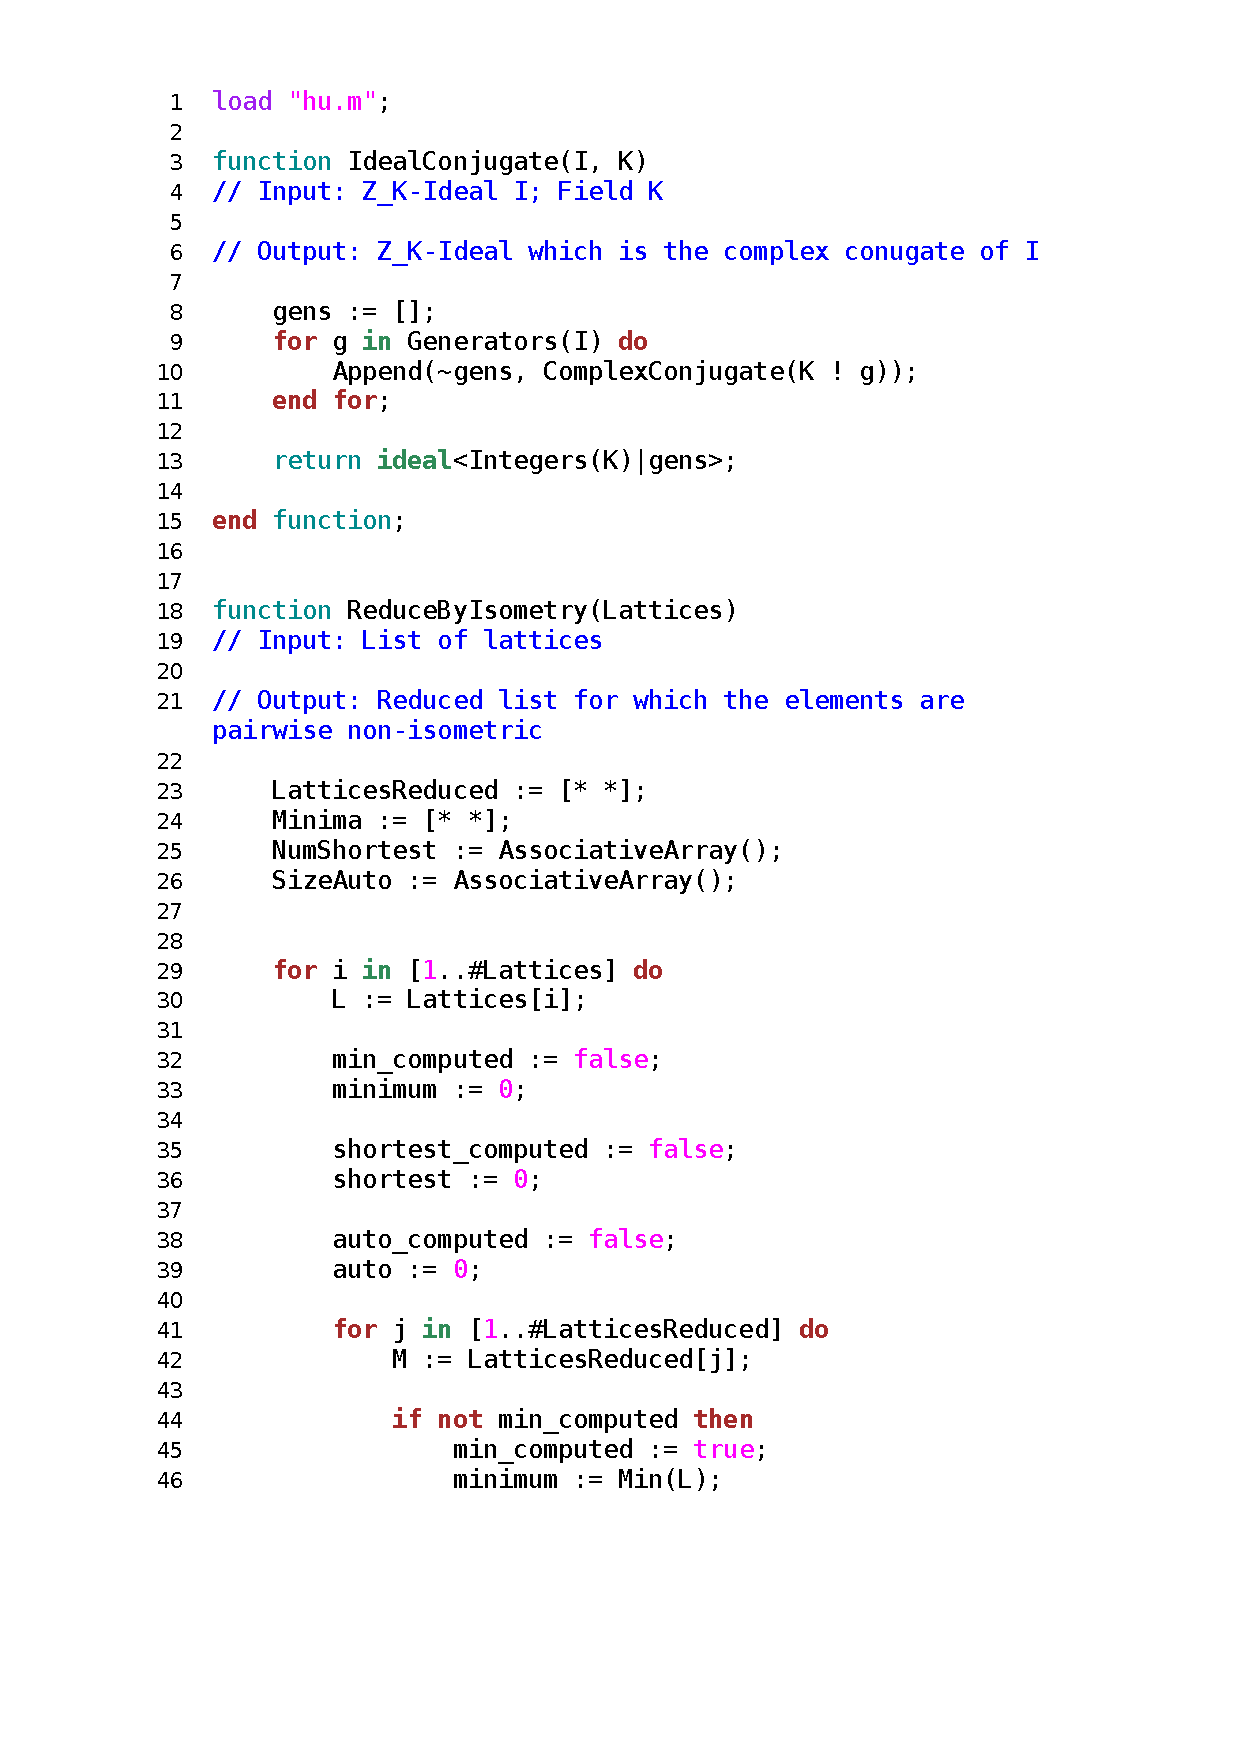
\includepdf[pages=-, pagecommand={}]{Utility.pdf}

\section{\texttt{MAGMA}-Implementierungen der Ideal-Gitter-Algorithmen}
Es folgt der Quellcode zu den Algorithmen aus Kapitel 3. Die implementierten Funktionen sind in der Reihenfolge des Quellcodes:
\begin{itemize}
	\item Alle Teiler eines $\Z_K$-Ideals $\I$ von festgelegter Norm berechnen. Siehe Algorithmus \eqref{alg:divnorm}.
	\item Einen total-reellen Erzeuger eines $\Z_K$-Ideals $\I$ bestimmen. Siehe Algorithmus \eqref{alg:relgen}.
	\item Matrix, deren Einträge die Vorzeichen der reellen Einbettung der Grundeinheiten kodieren sowie eine Liste aller total-positiven Elemente in $\Z_{K^+}^\ast$ reduziert nach $\lbrace \lambda \overline{\lambda} \mid \lambda \in \Z_K^\ast \rbrace$ und eine Liste von Erzeugern einer Untergruppe von $\Z_{K^+}^\ast$ mit ungeradem Index bestimmen. Siehe Algorithmus \eqref{alg:posgen}
	\item Das Minimalpolynom der Operation eines Automorphismus $\sigma$ von einem Gitter $L$ auf dem $\F_p$-Vektorraum $L^{\#,p}/L$ berechnen
	\item Liste aller total-positiven Erzeuger eines $\Z_K$-Ideals $\I$ reduziert nach $\lbrace \lambda \overline{\lambda} \mid \lambda \in \Z_K^\ast \rbrace$ bestimmen. Siehe ebenfalls Algorithmus \eqref{alg:posgen}.
	\item Liste von Vertretern der Klassengruppe von $K$ modulo der Operation der Galoisgruppe $\text{Gal}(K/\Q)$ bestimmen. Siehe Abschnitt (3.3).
	\item Aus einem $\Z_K$-Ideal $\I$ und einem total-positiven Element $\alpha$ das Gitter, welches durch Auffassung von $\I$ als $\Z$-Gitter mit Bilinearform $b(x,y) := \text{Spur}(\alpha x \overline{y})$ entsteht.
	\item Alle Ideal-Gittern über gegebenem CM-Körper mit vorgegebener Determinante und quadratfreier Stufe aufzählen. Siehe Algorithmus \eqref{alg:idlat}.
	\item Liste von allen $\ell$-modularen Gittern in Dimension $n$ erstellen, welche einen Automorphismus $\sigma$ besitzen mit $\mu_\sigma = \Phi_m$ und $\varphi(m) = n$. Siehe Abschnitt (3.5).
	\item Schleife, welche die letzte Funktion für verschiedene $n$ und $\ell$ auswertet und die Ergebnisse speichert.
\end{itemize}
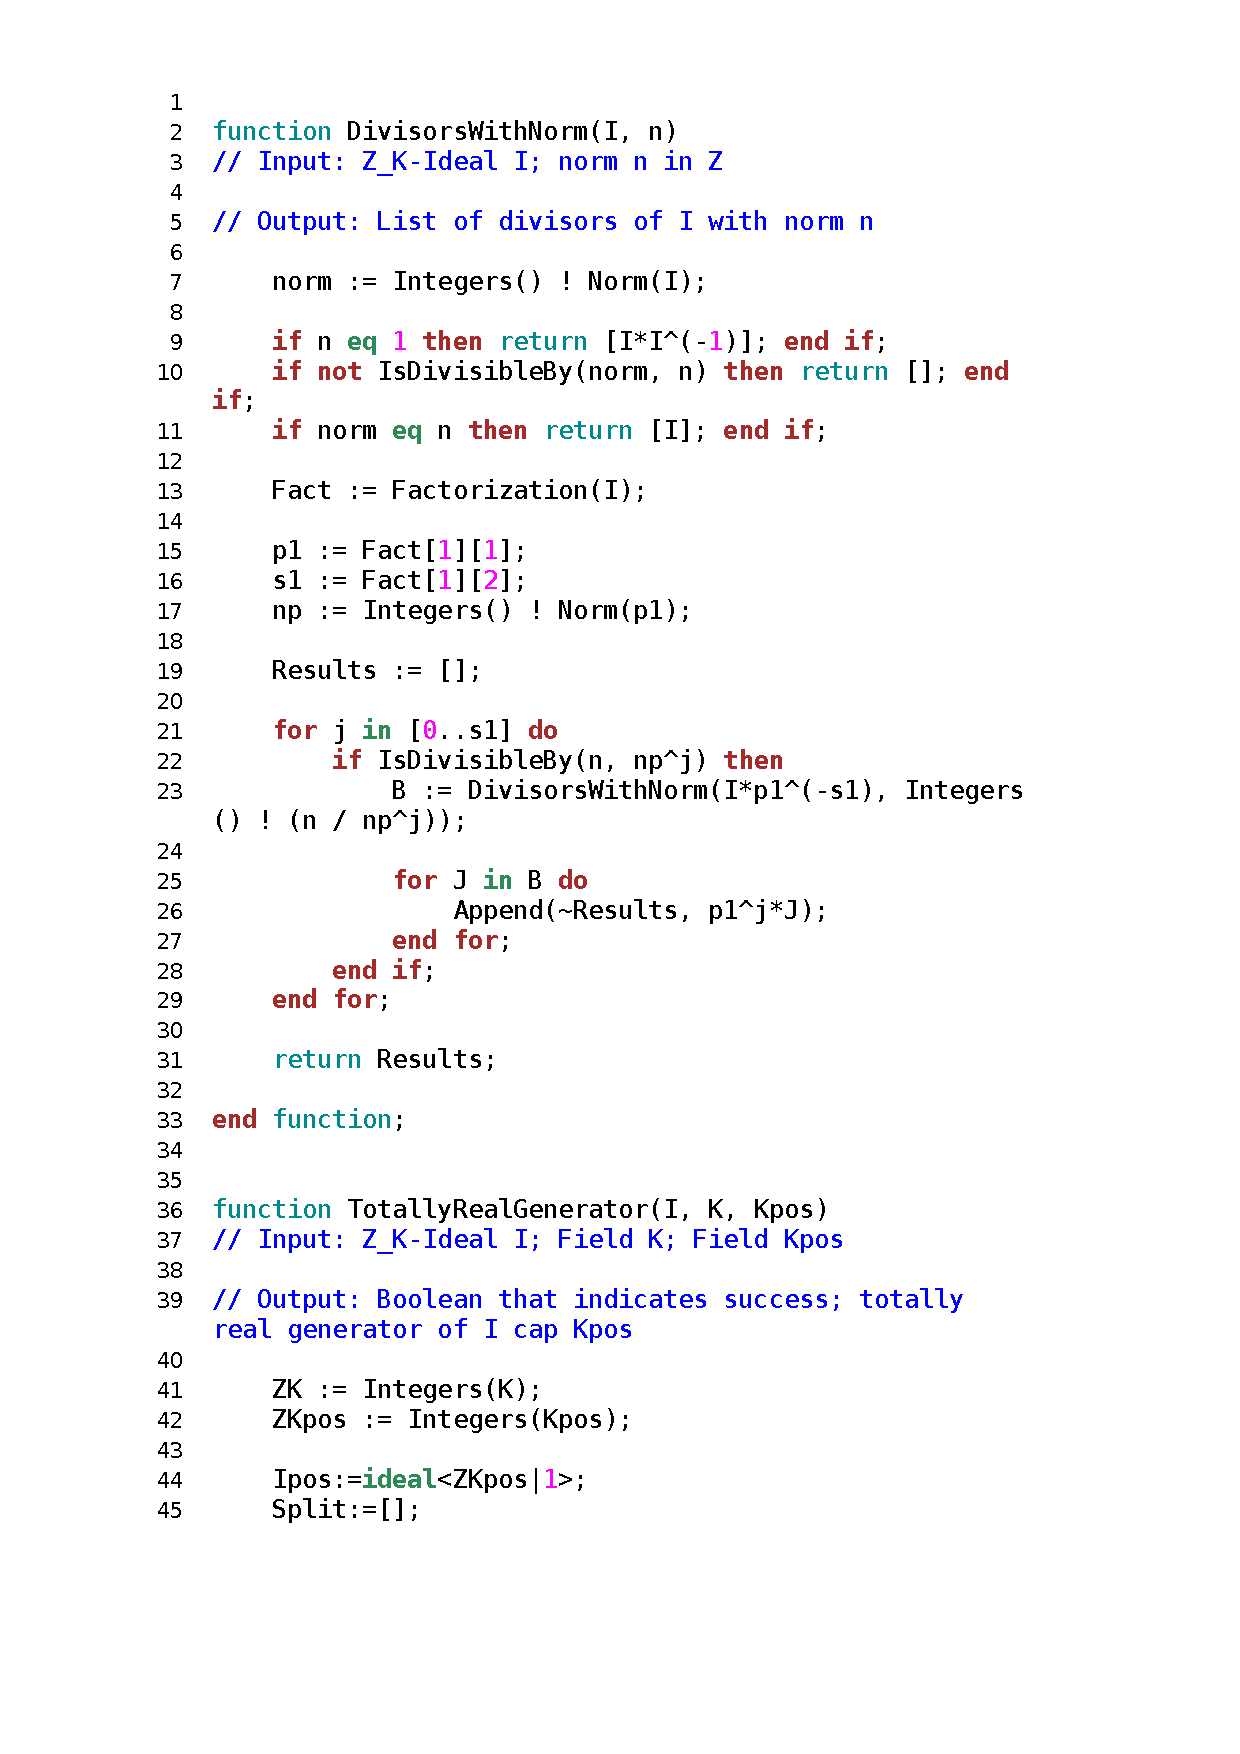
\includepdf[pages=-, pagecommand={}]{IdealLattices.pdf}

\section{\texttt{MAGMA}-Implementierungen der Subideal-Gitter-Algorithmen}
Es folgt der Quellcode zu den Algorithmen aus Kapitel 4 bis einschließlich Abschnitt (4.6). Die implementierten Funktionen sind in der Reihenfolge des Quellcodes:
\begin{itemize}
	\item Mithilfe von Hermite-Schranken die möglichen Typen von Automorphismen von Primzahlordnung gerader Gitter mit quadratfreier Stufe $\ell$, Determinante $\ell^k$ und Minimum $\geq t$ aufzählen. Siehe Algorithmus \eqref{alg:autotypes}.
	\item Mit dem Kneser'schen Nachbarverfahren die Vertreter der Isometrieklassen aller Gitter in dem Geschlecht eines Vertreters bestimmen. Siehe Algorithmus \eqref{alg:knesneigh}.
	\item Anhand von vorgegebener Dimension und Determinante Vertreter aller Isometrieklassen von (wenn gewünscht geraden) Gittern mit dieser Dimension und Determinante und mit quadratfreier Stufe aufzählen.
	\item Zu einem vorgegebenen Geschlechtssymbol Vertreter aller Isometrieklassen von Gittern mit diesem Geschlechtssymbol und quadratfreier Stufe aufzählen.
	\item Mit der \texttt{MAGMA}-Methode \texttt{Sublattices} $\sigma$-invariante Obergitter von Index $p^s$ für einen Gitterautomorphismus $\sigma$ bestimmen.
	\item Mit der in Abschnitt (4.5) beschriebenen Methode Obergitter von $L_1 \perp L_p$ invariant unter $\text{diag}(\sigma_1, \sigma_p)$ bestimmen. Siehe Algorithmus \eqref{alg:superlat}.
	\item Mit der Methode von Michael Jürgens alle Obergitter von $L$ mit Index $p^s$ bestimmen.
	\item Minimalpolynom der Operation eines Automorphismus $\sigma$ von einem Gitter $L$ auf dem $\F_p$-Vektorraum $L^{\#,p} / L$ bestimmen. Siehe Abschnitt (4.6).
	\item Liste aller extremalen $\ell$-modularen Gitter in Dimension $n$ bestimmen, die einen großen Automorphismus der Ordnung $m$ haben, sodass $m$ einen Primteiler $p$ mit $\ggT(p, \ell) = 1$ und $\frac{\mu_\sigma}{\Phi_m} \vert (X^\frac{m}{p} - 1)$ besitzt. Siehe Algorithmus \eqref{alg:largeauto}.
	\item Schleife, welche die letzte Funktion für verschiedene $n$ und $\ell$ auswertet und die Ergebnisse speichert.
\end{itemize}
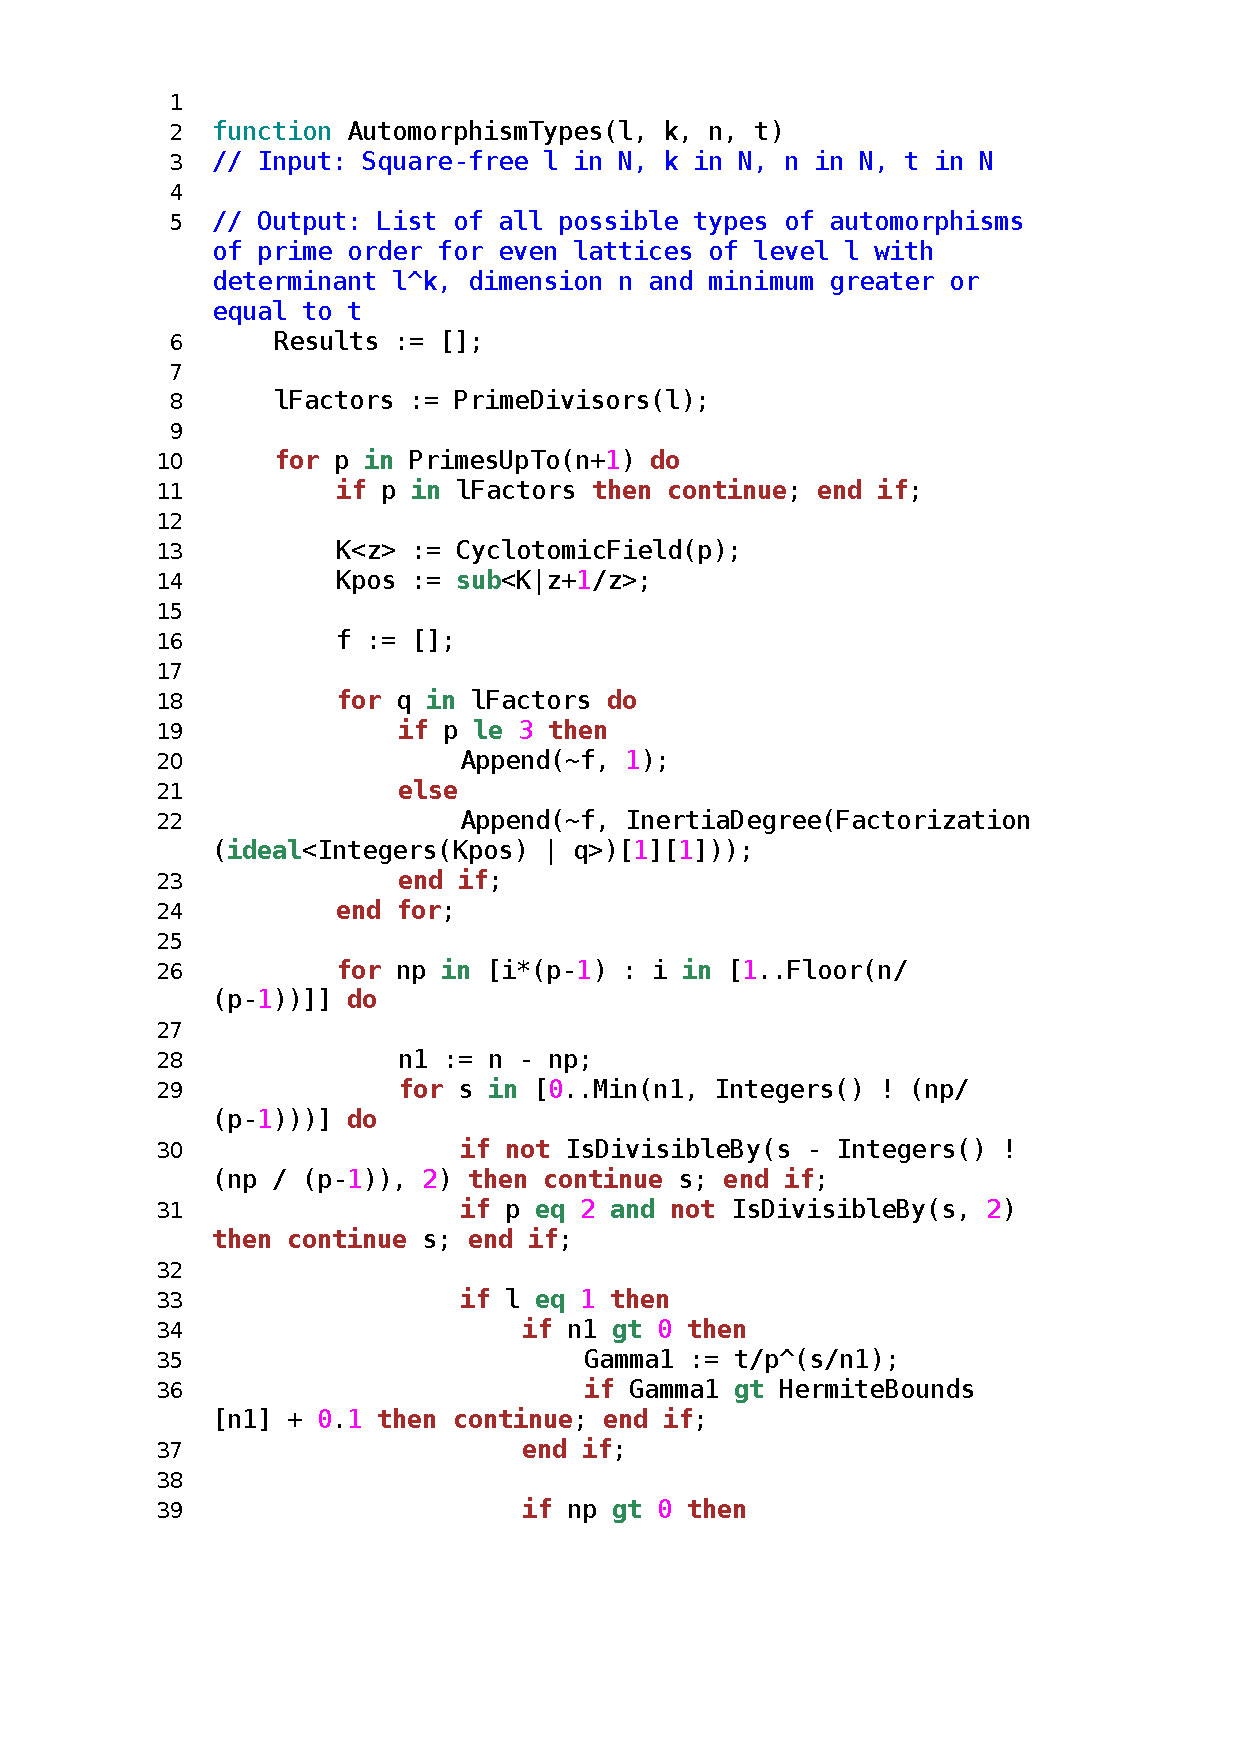
\includepdf[pages=-, pagecommand={}]{SubidealLattices.pdf}

\section{\texttt{MAGMA}-Implementierungen zur Aufzählung der charakteristischen Polynome}
Es folgt der Quellcode zu der Methode aus Abschnitt (4.7). Die implementierten Funktionen sind in der Reihenfolge des Quellcodes:
\begin{itemize}
	\item Einschränken der Möglichkeiten für Automorphismentypen extremaler modularer Gitter, indem versucht wird, Geschlechter von Bild- und Fixgitter mit Dimension $\leq 12$ aufzuzählen.
	\item Liste aller möglichen charakteristischen Polynome, die zu möglichen Automorphismentypen passende Partitionen des Raumes ergeben. Siehe Abschnitt (4.7).
\end{itemize}
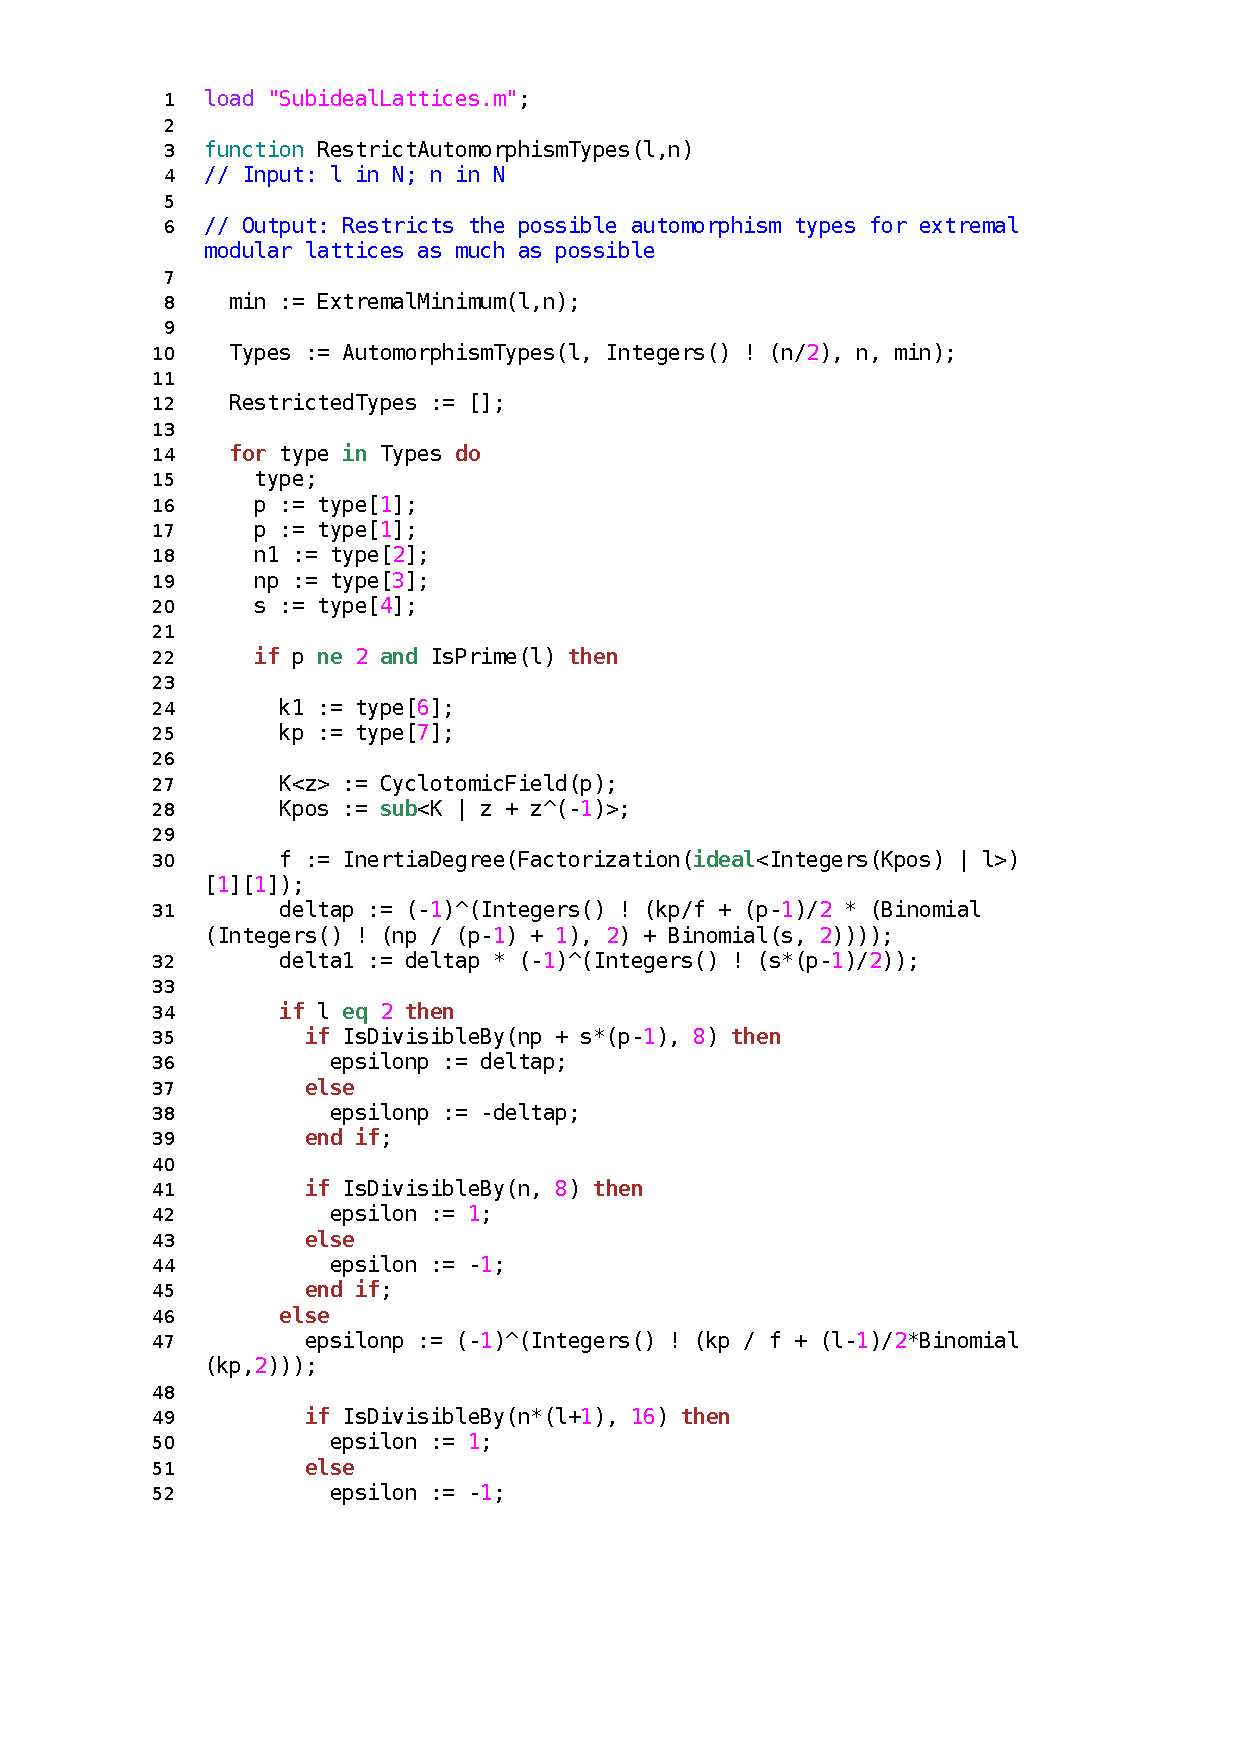
\includepdf[pages=-, pagecommand={}]{CharPols.pdf}

\newpage
\section{Eidesstattliche Versicherung}
Ich versichere hiermit an Eides Statt, dass ich die vorliegende Masterarbeit mit dem Titel
\textit{Extremale Gitter mit großen Automorphismen} selbstständig und ohne unzulässige fremde Hilfe erbracht habe.
Ich habe keine anderen als die angegebenen Quellen und Hilfsmittel benutzt. Die Arbeit hat in gleicher oder
ähnlicher Form noch keiner Prüfungsbehörde vorgelegen.\par
\vspace{0.5cm}
Aachen, im September 2018 \hfill $\underline{\hspace{6cm}}$\par
\vspace{2cm}
\begin{small}
\textbf{Belehrung:}\\
\textbf{§ 156 StGB: Falsche Versicherung an Eides Statt}\\
Wer vor einer zur Abnahme einer Versicherung an Eides Statt zuständigen Behörde eine solche Versicherung
falsch abgibt oder unter Berufung auf eine solche Versicherung falsch aussagt, wird mit Freiheitsstrafe
von bis zu drei Jahren oder mit Geldstrafe bestraft.\par
\textbf{§ 161 StGB: Fahrlässiger Falscheid; fahrlässige falsche Versicherung an Eides Statt}\\
(1) Wenn eine der in den §§ 154 bis 156 bezeichneten Handlungen aus Fahrlässigkeit begangen worden ist, so
tritt Freiheitsstrafe von bis zu einem Jahr oder Geldstrafe ein.\\
(2) Straflosigkeit tritt ein, wenn der Täter die falsche Angabe rechtzeitig berichtigt. Die
Vorschriften des § 158 Abs. 2 und 3 gelten entsprechend\par
\end{small}
Die vorstehende Belehrung habe ich zur Kenntnis genommen:\par
\vspace{0.5cm}
Aachen, im September 2018 \hfill $\underline{\hspace{6cm}}$\\

%===================================================================
% Literatur
%===================================================================
\newpage
\bibliography{Quellen}

\end{document}
